
\documentclass[11pt,a4paper]{book}
\usepackage[francais]{babel}
\usepackage{supertabular}
\usepackage{gensymb}
\usepackage{amsfonts,amssymb,amsmath,amsthm}
\usepackage{multicol,multirow}
\usepackage{comment}
\usepackage{accents}
\usepackage[utf8]{inputenc}  
\usepackage[T1]{fontenc} 
\usepackage[noadjust]{cite}
\usepackage{subfigure,epsfig}
\usepackage{longtable}
\usepackage{color}
\usepackage{atlasphysics}
\usepackage{feynmp}
\DeclareGraphicsRule{*}{mps}{*}{} 
\usepackage{arydshln}
%\usepackage{subfig}

\hoffset=-1.8cm
\textwidth=16cm
\voffset=-0.5cm
\textheight=23cm
\oddsidemargin=1.8cm
\evensidemargin=1.8cm
\linespread{1.}

\usepackage{fancyhdr}
\pagestyle{fancy}
\fancyhf{}
\fancyhead[LE,RO]{\thepage}

\renewcommand{\arraystretch}{1.4}

\setcounter{secnumdepth}{5}

\newenvironment{maliste}%
{ \begin{list}%
	{$\bullet$}%
	{\setlength{\labelwidth}{30pt}%
	 \setlength{\leftmargin}{35pt}%
	 %\setlength{\itemsep}{\parsep}
	 \setlength{\itemsep}{-0pt}	
	}
}%
{ \end{list} }

\newcommand{\fig}[1]{\vspace*{1.5cm}\begin{center}FIGURE: #1\end{center}\vspace*{1.5cm}}
\newcommand{\dd}{\ensuremath{{\rm d}}}
\newcommand{\dr}{\partial}
\newcommand{\ATLAS}   {ATLAS}
\newcommand{\english}[1]{{\it #1}}
\newcommand{\alpgen}  {{\sc Alpgen}}
\newcommand{\madgraph}  {{\sc MadGraph}}
\newcommand{\bridge}  {{\sc BRIDGE}}
\newcommand{\pythia}  {{\sc Pyth\-ia}}
\newcommand{\Perugia} {{\sc Perugia}}
\newcommand{\geant}   {G{\sc eant}4}
\newcommand{\herwig}  {{\sc Herwig}}
\newcommand{\herwigpp}{{\sc Herwig++}}
\newcommand{\jimmy}   {{\sc Jimmy}}
\newcommand{\blabla}{\textcolor{red}{\bf BLABLABLA}}
\newcommand{\exemples}{\textcolor{red}{\bf EXEMPLES}}
\newcommand{\insitu}{\english{in-situ}}
\newcommand{\antikt}{anti-$k_t$}
\newcommand{\Dzero}{D\O\ } 
\newcommand{\EM}    {{\rm EM}}
\newcommand{\EMJES} {{\rm EM+JES}}
\newcommand{\GCW}   {{\rm GCW}}
\newcommand{\LCW}   {{\rm LCW}}
\newcommand{\GSL}   {{\rm GSL}}
\newcommand{\GS}    {{\rm GS}}
%\newcommand{\GSC}    {{\rm GSC}}
\newcommand{\JES} {{\rm JES}}
\newcommand{\Response}  {\ensuremath{\mathcal{R}}} 
\newcommand{\ptjet}  {\ensuremath{\pt^\mathrm{jet}}}
\newcommand{\pttrue}  {\ensuremath{\pt^\mathrm{truth}}}
\newcommand{\Etruth}    {\ensuremath{E^{\rm truth}}}
\newcommand{\Ecalo}     {\ensuremath{E^{\rm jet}}}
\newcommand{\width}   {{\rm\it width}}
\newcommand{\HEC}    {\texttt{HEC}}
\newcommand{\LAr}    {\texttt{LAr}}
\newcommand{\FCal}   {\texttt{FCal}}
\newcommand{\Tile}   {\texttt{Tile}}
\newcommand{\Presampler}   {\texttt{PS}}
\newcommand{\ftile}{\ensuremath{f_{\Tile 0}}}
\newcommand{\fem}  {\ensuremath{f_{\LAr 3}}}
\newcommand{\fpres}{\ensuremath{f_{\rm PS}}}
\newcommand{\fhec} {\ensuremath{f_{\HEC 0}}}
\newcommand{\ffcal}{\ensuremath{f_{\FCal 1}}}
\newcommand{\etaRange}[2]{\ensuremath{{#1}\leq|\eta|<{#2}}}
\newcommand{\Lh}{{\cal L}}
\newcommand{\Lhm}{\ensuremath{{\cal L}_\text{m}}}
\newcommand{\Est}[1]{\hat{#1}}
\newlength{\dhatheight}
\newcommand{\EstCond}[1]{%
    \settoheight{\dhatheight}{\ensuremath{\hat{#1}}}%
    \addtolength{\dhatheight}{-0.2ex}%
    \hat{\vphantom{\rule{1pt}{\dhatheight}}%
    \smash{\hat{#1}}}}
\newcommand{\histfactory}{{\sc HistFactory}}
\newcommand{\opthylic}{{\sc OpTHyLiC}}
\newcommand{\tifosi}{{\sc TiFoSi}}
\newcommand{\mclimit}{{\sc McLimit}}
\newcommand{\roostats}{{\sc RooStats}}
\newcommand{\roofit}{{\sc RooFit}}
\newcommand{\rootcern}{{\sc ROOT}}
\newcommand{\tevatron}{Tevatron}
\newcommand{\CLs}{\ensuremath{CL_s}}
\newcommand{\CLsb}{\ensuremath{CL_{s+b}}}
\newcommand{\CLb}{\ensuremath{CL_b}}
\newcommand{\mup}{\ensuremath{\mu_{\text{up}}}}
\newcommand{\qmu}{\ensuremath{q_\mu}}
\newcommand{\qmup}{\ensuremath{q_{\mu_\text{up}}}}
\newcommand{\qmuobs}{\ensuremath{\qmu^{\text{obs}}}}
\newcommand{\qmupobs}{\ensuremath{\qmup^{\text{obs}}}}
\newcommand{\posterior}{{\it a posteriori}}
\newcommand{\prior}{{\it a priori}}
\newcommand{\scc}{\ensuremath{s_c}}
\newcommand{\scck}{\ensuremath{s_{cl}}}
\newcommand{\bc}{\ensuremath{b_{c}}}
\newcommand{\bck}{\ensuremath{b_{cl}}}
\newcommand{\bci}{\ensuremath{b_{ci}}}
\newcommand{\bcik}{\ensuremath{b_{cil}}}
\newcommand{\scnom}{\ensuremath{\scc^{\text{nom}}}}
\newcommand{\scknom}{\ensuremath{\scck^{\text{nom}}}}
\newcommand{\bcinom}{\ensuremath{\bci^{\text{nom}}}}
\newcommand{\bciknom}{\ensuremath{\bcik^{\text{nom}}}}
\newcommand{\bcnom}{\ensuremath{\bc^{\text{nom}}}}
\newcommand{\bcknom}{\ensuremath{\bck^{\text{nom}}}}
\newcommand{\s}{\ensuremath{s}}
\newcommand{\snom}{\ensuremath{s^{\text{nom}}}}
\newcommand{\bnom}{\ensuremath{b^{\text{nom}}}}
\newcommand{\back}{\ensuremath{b}}
\newcommand{\bi}{\ensuremath{b_i}}
\newcommand{\nobsc}{\ensuremath{\nobs_c}}
\newcommand{\nobsck}{\ensuremath{\nobs_{cl}}}
\newcommand{\nobs}{\ensuremath{N^{\text{obs}}}}
\newcommand{\n}{\ensuremath{N}}
\newcommand{\nc}{\ensuremath{N_{c}}}
\newcommand{\nck}{\ensuremath{N_{cl}}}
\newcommand{\E}[1]{\ensuremath{\mathbb{E}\left[#1\right]}}
\newcommand{\fsyst}{\ensuremath{h^{\text{syst}}}}
\newcommand{\ffup}{\ensuremath{h^{\uparrow}}}
\newcommand{\ffdown}{\ensuremath{h^{\downarrow}}}
\newcommand{\pval}{\english{p-value}}
\newcommand{\nochan}{\ensuremath{n}}
\def\fourtop{\ensuremath{t\bar{t}t\bar{t}}}

\begin{document}

\begin{titlepage}
\vspace*{-3cm}
\flushright{PCCF T 1512}

\vspace*{3.2cm}

\begin{center}
\noindent {\Large \textbf{Universit\'e Blaise Pascal}} \\
\vspace*{0.3cm}
\noindent {\Large \textbf{U.F.R. Sciences et Technologies}} \\
\vspace*{0.5cm}
\noindent \huge \textbf{Habilitation \`a Diriger des Recherches} \\
\vspace*{0.5cm}
\vspace*{0.4cm}
\noindent \large {Présentée par\\}
\vspace*{0.4cm}
\noindent \LARGE \textbf{Emmanuel \textsc{BUSATO}} \\
\vspace*{0.4cm}
\noindent \large {Docteur en physique de l'Universit\'e Denis Diderot (Paris 7)\\}
\vspace*{0.1cm}
\noindent \large {Ma\^itre de conf\'erence \`a l'Universit\'e Blaise Pascal (Clermont 2)\\}
\vspace*{0.8cm}
%\noindent {\LARGE \textbf{Test du Mod\`ele Standard sur collisionneur}} \\
\vspace*{0.4cm}
%\noindent {\LARGE \textbf{avec quark Top et boson de Higgs}} \\

\vspace*{0.5cm}
\noindent \LARGE \textbf{Calibration des jets, recherche de nouvelle physique et interpr\'etation statistique avec les donn\'ees de l'exp\'erience ATLAS au run 1 du LHC} \\
\vspace*{0.5cm}

\vspace*{0.8cm}
\noindent \Large  \\
\vspace*{0.6cm}
\noindent \large Travaux pr\'esent\'es le 17 d\'ecembre 2015 devant le jury compos\'e de :
\vspace*{0.2cm}
\end{center}
\begin{center}
\noindent \large
\begin{tabular}{llcl}
\textit{Rapporteurs :}    & Philippe \textsc{Rosnet}         & - &  Professeur, Universit\'e Blaise Pascal (LPC)\\
                          & Mossadek \textsc{Talby}          & - &  Professeur, Universit\'e Aix Marseille (CPPM)\\
                          & Isabelle \textsc{Wingerter-Seez} & - &  Directrice de Recherche (LAPP)\\
%\textit{Président :}     & Alain \textsc{Falvard}           & - &  Directeur de Recherche (LPC)\\
\textit{Examinateurs :}   & Laurent \textsc{Derome}          & - &  Professeur, Universit\'e Joseph Fourier (LPSC)\\
                          & Alain \textsc{Falvard}           & - &  Directeur de Recherche (LPC)\\
                          & Domnique \textsc{Pallin}         & - &  Directeur de Recherche (LPC)

\end{tabular}
\end{center}
\end{titlepage}
\sloppy

\titlepage



\chapter*{Remerciements}

Je tiens \`a remercier tout d'abord les membres du jury pour l'int\'er\^et qu'ils ont 
port\'e \`a mon travail et pour leurs commentaires et suggestions lors de la pr\'eparation 
de ce manuscrit et de la soutenance. Merci \`a Philippe Rosnet, Isabelle Wingerter-Seez et
Mossadek Talby 
pour leur travail de rapporteur, leur lecture attentive du manuscrit et leurs remarques. 
Un grand merci \'egalement \`a Laurent Derome pour avoir accept\'e de participer au jury et pour ses remarques 
utiles sur les statistiques. 

Je remercie Alain Falvard et Dominique Pallin de m'avoir pouss\'e \`a passer cette habilitation. 
Je remercie \'egalement mon p\`ere qui a fortement contribu\'e \`a me convaincre lui aussi. C'est 
certainement chose utile dans notre syst\`eme de recherche d'avoir la HDR, m\^eme si le sens profond 
de ce dipl\^ome m'\'echappe toujours ! 

Je remercie tous les membres de l'\'equipe ATLAS du LPC avec qui il a \'et\'e tr\`es agr\'eable de 
travailler toutes ces ann\'ees. Il m'est impossible de remercier tous les physiciens et physiciennes 
qui ont contribu\'e de pr\`es ou de loin aux travaux pr\'esent\'es ici et je 
me contenterai donc de citer ceux dont la contribution a \'et\'e la plus forte. Merci donc aux 
chefs de groupe Fran\c cois Vazeille et Dominique Pallin pour la libert\'e qu'ils m'ont laiss\'ee dans 
mes recherches et la bonne atmosph\`ere de travail qu'ils ont su instaurer dans le groupe. Merci \`a Reina 
Camacho pour la super p\'eriode que nous avons pass\'e \`a travailler sur les jets. Le 
chapitre~\ref{chap:calibjets} est avant tout le fruit de son travail. C'est une chance immense pour moi de 
l'avoir eu comme premi\`ere doctorante. Merci \`a David Calvet sans qui les travaux 
pr\'esent\'es dans les chapitres~\ref{chap:OTHandTIFOSI} et \ref{chap:Recherche4tops} n'auraient pas 
\'et\'e possibles. C'est l\`a aussi une grande chance pour moi d'avoir pu collaborer avec lui sur ces 
sujets.

Finalement, je tiens \`a remercier l'ensemble des membres du LPC, de l'universit\'e Blaise Pascal et 
d'ailleurs qui m'ont aid\'e \`a un moment ou \`a un autre, que ce soit dans mes activit\'es de recherche 
ou d'enseignement.  



\tableofcontents

\mainmatter

\chapter*{Introduction}
\addcontentsline{toc}{chapter}{Introduction}

Ce document r\'esume mes activit\'es de recherche sur l'exp\'erience \ATLAS{} durant le run 1 du LHC. 
Ce run, qui s'est d\'eroul\'e de fin 2009 \`a d\'ebut 2013, correspond \`a la premi\`ere phase de fonctionnement du collisionneur et donc \`a la premi\`ere phase de prise de donn\'ees de l'exp\'erience \ATLAS. 
Il est le premier d'une longue s\'erie qui devrait s'\'ecouler jusqu'en 2030 environ. 
L'\'etude des donn\'ees enregistr\'ees durant le run 1 a permis de r\'ealiser les premi\`eres \'etudes de performance du d\'etecteur apr\`es pr\`es de vingt ann\'ees de R\&D et de construction, 
et a conduit, en 2012, \`a la d\'ecouverte d'un boson scalaire compatible avec le boson BEH. 
Elle a aussi permis  
de r\'ealiser les premi\`eres recherches de ph\'enom\`enes non-pr\'edits par le mod\`ele standard \`a $\sqrt{s}>1.96$~TeV, qui était l'\'energie maximale sond\'ee jusqu'alors gr\^ace au Tevatron et aux exp\'eriences \Dzero et CDF.

Au d\'ebut du run 1, mon activit\'e a port\'e sur la mesure de l'\'energie des jets et plus particuli\`erement sur l'\'etude des performances d'une m\'ethode de calibration permettant %, 
%par l'application de corrections relativement simples, 
une am\'elioration significative de la r\'esolution en \'energie et une r\'eduction importante de l'incertitude syst\'ematique li\'ee \`a la saveur du parton donnant naissance au jet. Ce travail est d\'ecrit dans le chapitre~\ref{chap:calibjets}.

Par la suite mon activit\'e s'est focalis\'ee sur la recherche d'une signature nouvelle de physique au-del\`a du mod\`ele standard : les \'ev\'enements avec quatre quarks top dans l'\'etat final. 
Cette recherche 
%est nouvelle dans le sens o\`u elle 
n'\'etait pas possible au Tevatron du fait de la trop faible \'energie dans le r\'ef\'erentiel du centre de masse. Gr\^ace aux donn\'ees recueillies par l'exp\'erience \ATLAS{} \`a $\sqrt{s}=7$~et~$8$~TeV, 
nous avons 
%ainsi 
pu contraindre des mod\`eles sur lesquels il n'existait pas (ou peu) de contraintes. 
Mon travail a notamment port\'e sur l'interpr\'etation statistique des donn\'ees et plus particuli\`erement sur les m\'ethodes utilis\'ees pour calculer les limites d'exclusion. 
Il a conduit, entre autre, au d\'eveloppement d'outils sp\'ecialis\'es pouvant \^etre utilis\'es pour toute recherche de processus poissonniens. Ces outils sont introduits et d\'ecrits dans les chapitres~\ref{chap:interpretationStatLimit} et \ref{chap:OTHandTIFOSI}. La recherche d'\'ev\'enements avec quatre quarks top ainsi que les r\'esultats obtenus sont d\'ecrits dans le chapitre~\ref{chap:Recherche4tops}.

Les travaux et r\'esultats pr\'esent\'es dans ce document ne sont bien-s\^ur par le fait de mon seul travail. Il s'agit \`a chaque fois de la production d'un groupe de personnes et notamment des doctorants ayant travaill\'es sur ces diff\'erents sujets. Ces personnes (au moins celles avec qui j'ai le plus travaill\'e) seront cit\'ees d\`es qu'il se doit au sein de ce document.



\chapter{Calibration des jets avec les premi\`eres donn\'ees du run 1}
\label{chap:calibjets}

De tr\`es nombreux processus \'etudi\'es au LHC conduisent \`a la production de quarks et de gluons dans l'\'etat final de la collision. 
Une fois produits, les quarks et gluons s'hadronisent pour donner des jets collim\'es de particules sans couleur. 
Ces particules interagissent dans le d\'etecteur et les signaux produits, une fois regroup\'es en jets dits calorim\'etriques \`a l'aide d'un algorithme de reconstruction, constituent la signature exp\'erimentale des quarks et des gluons. 

La mesure des jets calorim\'etriques est fauss\'ee par plusieurs effets tels que la non-compensation des calorim\`etres, les pertes d'\'energies dans les parties non-instrument\'ees du d\'etecteur, les inefficacit\'es de reconstruction, etc.. 
%Ces effets doivent \^etre corrig\'es pour permettre une mesure pr\'ecise des processus physiques conduisant \`a la production de jets. 
L'ensemble des corrections appliqu\'ees pour corriger ces effets forment la calibration des jets. 
Avoir une calibration des jets pr\'ecise est crucial car elle est souvent une source d'incertitude importante lors de la mesure des processus physiques, comme 
par exemple lors des mesures des sections efficaces de production d'\'ev\'enements di-jets ou multijets~\cite{Aad:2014vwa,Aad:2013tea}, d'\'ev\'enements $t\bar{t}$~\cite{Aad:2014iaa} ou encore lors de la recherche de nouvelles r\'esonances se d\'esint\'egrant~en~jets~\cite{Aad:2014aqa}. 

%Les jets r\'esultants de l'hadronisation des quarks et gluons sont produits en grande quantit\'e dans les collisions de protons au LHC. Leur pr\'esence est exploit\'ee pour de nombreuses mesures et recherches de nouvelle physique. L'incertitude sur la mesure de l'\'energie des jets est, pour beaucoup d'entre elles, l'incertitude exp\'erimentale dominante. C'est le cas par exemple des mesures de section efficace de production d'\'ev\'enements di-jets ou multijets~\cite{Aad:2014vwa,Aad:2013tea}, d'\'ev\'enements top-antitop~\cite{Aad:2014iaa} ou encore de la recherche de nouvelles r\'esonances se d\'esint\'egrant en jets~\cite{Aad:2014aqa}. Avoir une mesure pr\'ecise de l'\'energie des jets est par cons\'equent d\'eterminant dans le programme de physique de l'exp\'erience \ATLAS. 

La stratégie d'\ATLAS~au début du run 1 était de mettre en place une calibration simple et robuste (nommée \EMJES) qui puisse être utilisée dans les analyses de physique rapidement et de développer en parallèle des calibrations plus sophistiquées qui pourraient, si elles s'avéraient performantes, être utilisées dans les analyses ultérieures. Une partie de mes travaux entre 2009 et 2012 a port\'e sur le d\'eveloppement d'une de ces m\'ethodes "sophistiqu\'ees" appel\'ee \english{Global Sequential}  (\GS) \english{Calibration}. Cette m\'ethode utilise les jets calibr\'es \`a l'\'echelle \EMJES~et leur applique des corrections suppl\'ementaires dans le but d'am\'eliorer leur r\'esolution en \'energie et de s'affranchir d'une partie de la d\'ependance avec la saveur. La reconstruction des jets et la calibration \EMJES~sont d\'ecrits succintement dans les sections \ref{sec:jetReco} et \ref{sec:EMJES}. La calibration \GS~est d\'ecrite dans la section \ref{sec:GS}. Ses performances et sa validation sur les donn\'ees sont d\'ecrites dans les sections~\ref{sec:performanceGS} et \ref{sec:systUncertGS}.

Les résultats pr\'esent\'es dans ce chapitre sur la calibration \GS{} sont le fruit d'un travail collectif r\'ealis\'e avec Reina Camacho, doctorante dans le groupe \ATLAS~du LPC entre 2009 et 2012 ayant travaill\'e sur cette calibration pendant la premi\`ere moiti\'e de sa th\`ese \cite{camacho:tel-00747143} et David Lopez Mateos et Ariel Schwartzman, initiateurs de cette calibration au sein d'\ATLAS. Ils sont pour la plupart tir\'es de la note~\cite{Busato:1365519} et de l'article~\cite{Aad:2011he}. Ce chapitre refl\`ete l'\'etat de la calibration des jets dans \ATLAS~\`a l'\'epoque o\`u cet article a \'et\'e \'ecrit et non celui au moment o\`u le pr\'esent document est publi\'e.

Dans ce qui suit, les résultats sur les données ont été obtenus sur le lot recueilli en 2010 à $\sqrt{s}=7~$TeV. La luminosité intégrée est de $38$~pb$^{-1}$. 

\section{Reconstruction des jets}
\label{sec:jetReco}

Les jets sont reconstruits par l'algorithme \antikt~\cite{Cacciari:2008gp} avec un param\`etre de distance $R=0,4$ ou $R=0,6$. Les objets utilis\'es en entr\'ee sont soit les amas dit "topologiques" reconstruits \`a partir des cellules des calorim\`etres \'electromagn\'etiques et hadroniques d'ATLAS~\cite{1748-0221-3-08-S08003}, soit les tours calorim\'etriques, soit les particules g\'en\'er\'ees dans le cas d'\'ev\'enements simul\'es. Dans ce qui suit, seuls les r\'esultats pour $R=0,6$ et pour les jets calorim\'etriques construits \`a partir des amas topologiques sont pr\'esent\'es. 

Les amas topologiques sont construits en regroupant les cellules voisines dont le rapport signal/bruit est grand. Leur utilisation permet de r\'eduire l'impact du bruit sur la reconstruction des jets et de l'\'energie transverse manquante et donc d'am\'eliorer les performances en terme d'identification et de r\'esolution. De plus, ils permettent une d\'efinition et une calibration des jets plus naturelle que celles obtenues avec les tours car ils sont l'image dans le calorim\`etre des gerbes \'electromagn\'etiques et hadroniques. %Le principe de l'algorithme de reconstruction des amas topologique est h\'erit\'e de l'algorithme "T42" de l'exp\'erience \Dzero \cite{D0noteUrsula, D0noteGregEmmJR, vlimantThesis, busatoThesis}, lui-m\^eme h\'erit\'e de l'exp\'erience H1. 

Apr\`es reconstruction, les jets calorim\'etriques sont \`a l'\'echelle dite \'electromagn\'etique (\EM). Cette \'echelle, d\'etermin\'ee par des tests en faisceaux, est telle que la r\'eponse est \'egale \`a 1 pour des \'electrons. 

Pour les \'ev\'enements simul\'es, les jets form\'es par les particules g\'en\'er\'ees sont reconstruits en utilisant le m\^eme algorithme que pour les jets calorim\'etriques. Toute les particules dont le temps de vie est sup\'erieur \`a 10~ps sont utilis\'ees \`a l'exception des muons et neutrinos. Ces jets servent de r\'ef\'erence dans les calibrations \EMJES~et \GS. Nous les appelerons par la suite les "jets de particules".

\section{Calibration \EMJES}
\label{sec:EMJES}

 La calibration \EMJES~corrige l'\'energie des jets calorim\'etriques de telle sorte \`a la ramener, en moyenne, \`a l'\'energie des jets de particules. Ceci a pour effet d'amener l'\'energie des jets \`a une \'echelle hadronique et donc de corriger 
%en partie 
la non-compensation des calorim\`etres \'electromagn\'etiques et hadroniques, les pertes d'énergies dans les parties non-instrumentées du détecteur, les inefficacités de reconstruction des amas topologiques, etc.. La direction des jets est \'egalement chang\'ee pour tenir compte de la position du vertex primaire et pour corriger du biais en $\eta$ provenant des d\'ep\^ots d'\'energie dans les r\'egions peu instrument\'ees du d\'etecteur. Cette calibration est d\'eriv\'ee sur un \'echantillon d'\'ev\'enements multi-jets simul\'es avec \pythia~(par la suite appel\'e \'echantillon nominal ou \'echantillon \pythia MC10) en fonction de la pseudorapidit\'e $\eta$ et de l'\'energie. Seuls les jets calorim\'etriques isol\'es associ\'es \`a un jet de particule isol\'e dans $\Delta R=3$ sont consid\'er\'es\footnote{$\Delta R=\sqrt{\Delta\eta^2+\Delta\phi^2}$}. Un jet est isol\'e si aucun autre jet d'impulsion transverse sup\'erieure \`a 7~GeV ne se trouve \`a moins de $\Delta R=2,5\times R$, o\`u $R$ est le param\`etre de distance de l'algorithme \antikt. 

La r\'eponse en \'energie
\[\langle\Response \rangle=\left<\frac{\Ecalo}{\Etruth}\right>\]
 \`a l'\'echelle \'electromagn\'etique est repr\'esent\'ee sur la figure \ref{fig:fig_09_responseEMscaleVsEta} en fonction de la pseudo-rapidit\'e pour diff\'erentes \'energies. Dans cette expression, $\Ecalo$ d\'esigne l'\'energie du jet calorim\'etrique, $\Etruth$ l'\'energie du jet de particule qui lui est associ\'e et $\left<\right>$ la moyenne sur les jets obtenue par un ajustement gaussien. Apr\`es calibration \EMJES, la r\'eponse est proche de 1. %Les facteurs correctifs \`a appliqu\'es pour atteindre un tel r\'esultat peuvent \^etre relativement grands. La figure \ref{fig:fig_09_responseEMscaleVsEta} montre que, \`a basse \'energie ils peuvent aller jusqu'\`a 2.

\begin{figure}[!h]
	\centering
	\includegraphics[scale=0.5]{figures/fig_09_responseEMscaleVsEta.pdf}
	\caption{R\'eponse en \'energie des jets \`a l'\'echelle \'electromagn\'etique en fonction de la pseudo-rapidit\'e pour diff\'erentes \'energies.}
	\label{fig:fig_09_responseEMscaleVsEta}
\end{figure}

L'incertitude sur l'\'echelle en \'energie \EMJES~provient de plusieurs sources :
\begin{maliste}
\item M\'ethode de calibration : cette incertitude est estim\'ee en appliquant la calibration sur l'\'echantillon utilis\'e pour la d\'eriver. 
\item R\'eponse en \'energie des calorim\`etres : cette incertitude est estim\'ee en propageant au jet l'incertitude sur la r\'eponse pour des hadrons isol\'es mesur\'ee soit \insitu~soit sur les donn\'ees du test en faisceau combin\'e de 2004.
\item Mod\'elisation du bruit dans les cellules calorim\'etriques : cette incertitude est estim\'ee en faisant varier le seuil sur le bruit dans la simulation
\item Mod\'elisation des mat\'eriaux dans le d\'etecteur : cette incertitude est estim\'ee en faiscant varier la quantit\'e de mat\'eriaux de diff\'erentes parties du d\'etecteur dans la simulation.
\item Mod\'elisation des \'ev\'enements dans les g\'en\'erateurs Monte Carlo : cette incertitude est estim\'ee en comparant la r\'eponse nominale (calcul\'ee sur l'\'echantillon \pythia~nominal) \`a la r\'eponse obtenue dans des \'echantillons simul\'es avec des mod\`eles de fragmentation, d'\'ev\'enement sous-jacent et de physique pour l'\'ev\'enement dur diff\'erent.
\end{maliste}

Les incertitudes associ\'ees \`a ces diff\'erentes sources ainsi que l'incertitude totale sont repr\'esent\'ees, pour la partie centrale du d\'etecteur, sur la figure \ref{fig:fig_22a_JES2010UncertaintyCentral}.

\begin{figure}[!h]
	\centering
	\includegraphics[scale=0.5]{figures/fig_22a_JES2010UncertaintyCentral.pdf}
	\caption{Incertitude syst\'ematique sur l'\'echelle en \'energie \EMJES~dans la partie centrale du d\'etecteur ($0,3\leq|\eta|<0,8$). Les contributions des diff\'erentes sources discut\'ees dans le texte sont montr\'ees, ainsi que l'incertitude totale (histogramme bleu).}
	\label{fig:fig_22a_JES2010UncertaintyCentral}
\end{figure}

\section{Calibration \GS}
\label{sec:GS}

La calibration \GS{} est une extension multivariée de la calibration EM+JES. Après la calibration EM+JES, la dépendance de la réponse avec $\eta$ et l'\'energie est supprimée. Cependant, la réponse peut dépendre d'autres variables comme celles caractérisant l'extension longitudinale et transversale des jets. La calibration \GS~supprime ces dépendances de manière séquentielle. Ses effets principaux sont d'am\'eliorer la résolution en énergie des jets et de réduire la dépendance de la réponse avec la saveur. 

Toute variable $x$ corr\'el\'ee avec la r\'eponse du calorim\`etre peut \^etre utilis\'ee. La r\'eponse en fonction de $x$ est d\'efinie par
\begin{equation} 
\label{eq:responsegsc}
                \langle \Response(x)  \rangle  =  \left<\frac{\ptjet(x)}{\pttrue}\right>
\end{equation}
o\`u \ptjet{} est l'impulsion transverse du jet calibr\'e \`a l'\'echelle \EMJES{} et \pttrue{} celle du jet de particule. Comme pour la calibration \EMJES{}, seuls les jets isol\'es associ\'es \`a un jet de particule isol\'e sont utilis\'es. La moyenne dans l'\'equation \ref{eq:responsegsc} est obtenue par ajustement gaussien dans un intervalle en  \pttrue, $\eta$ et $x$.

La d\'ependance de la r\'eponse en $x$ est supprim\'ee en multipliant $\ptjet$ par
\begin{equation}
\label{eq:gsc}
                C(x) = 1/ \langle \Response(x) \rangle.
\end{equation}
 
Plusieurs variables peuvent \^etre utilis\'ees de mani\`ere s\'equentielle pour atteindre la r\'esolution optimale. Cette proc\'edure requiert que la correction pour la variable $x_{n}$ soit calcul\'ee sur les jets pour lesquels les corrections pour les variables pr\'ec\'edentes aient d\'ej\`a \'et\'e appliqu\'ees. L'impulsion transverse d'un jet après la calibration \GS~est
\begin{equation}
\label{eq:ptGSaftercalib}
\pt^\GS=\left(\prod\limits_{n=1}^{N}C_n(x_n)\right)\times \pt^\EMJES
\end{equation}
où $N$ est le nombre de variables utilisées. Lors de l'application de cette procédure séquentielle, il faut prêter attention à ce que la correction pour la variable $n$ ne soit pas dégradée par les corrections $k>n$. Il a \'et\'e v\'erifi\'e que la r\'eponse en fonction de chaque variable ne change pas jusqu'\`a la derni\`ere correction. 

\subsection{Propri\'et\'es longitudinales et transversales des jets}

Les variables utilis\'ees dans la calibration \GS~(les $x_n$ dans l'\'equation \ref{eq:ptGSaftercalib}), sont des propri\'et\'es caract\'erisant la topologie longitudinale et transversale des d\'epots d'\'energie dans le jet. 
Une grande quantit\'e d'\'energie d\'epos\'ee dans les couches du calorim\`etre proches du point d'interaction indique que la gerbe a commenc\'e \`a se d\'evelopper en amont du calorim\`etre, induisant une r\'eponse plus faible puisqu'une partie de l'\'energie n'est pas d\'etect\'ee. 
Une grande fraction d'\'energie d\'epos\'ee dans le calorim\`etre hadronique indique une grande fraction hadronique au sein du jet conduisant \`a une r\'eponse plus faible (du fait de la non-compensation des calorimètres d'\ATLAS). 
Dans la partie centrale du d\'etecteur, une grande \'energie d\'epos\'ee dans la derni\`ere couche du calorim\`etre \'electromagn\'etique et dans la premi\`ere couche du calorim\`etre hadronique peut indiquer qu'une certaine fraction de l'\'energie du jet a \'et\'e perdue dans la partie non-instrument\'ee entre les deux calorim\`etres. 
La r\'eponse calorim\`etrique et l'extension transversale des jets sont corr\'el\'ees \`a la quantit\'e d'\'energie qui est perdue entre les parties tonneau et bouchon des calorim\`etres.

Chaque propri\'et\'e utilis\'ee peut \^etre sensible \`a plusieurs effets. Aucune tentative n'est faite pour s\'eparer ces effets dans la calibration \GS. Ils sont corrig\'es de mani\`ere implicite par les diff\'erentes corrections qui apparaissent dans l'\'equation \ref{eq:ptGSaftercalib}.

La structure longitudinale d'un jet (c'est-\`a-dire la structure le long de son axe), est caract\'eris\'ee par la fraction d'\'energie d\'epos\'ee dans les diff\'erentes couches des calorim\`etres \'electromagn\'etique et hadronique avant qu'une quelconque calibration en \'energie soit appliqu\'ee :
\begin{equation}
f_{\rm layer} = \frac{E_\EM^{\rm layer}}{E_\EM^{\rm jet}},
\end{equation}
o\`u $E_\EM^{\rm jet}$ est l'\'energie du jet \`a l'\'echelle \'electromagn\'etique et $E_\EM^{\rm layer}$ l'\'energie d\'epos\'ee dans la couche calorim\'etrique d'int\'er\^et, calcul\'ee \'egalement \`a l'\'echelle \'electromagn\'etique.

La structure transversale d'un jet (c'est-\`a-dire la structure dans le plan perpendiculaire \`a son axe) est d\'efinie par la largeur
\begin{equation}
\width = \frac{\displaystyle \sum_{i} p^i_{\rm T} \; \Delta R_{i,{\rm jet}}} {\displaystyle \sum_{i} p^i_{\rm T}},
\label{eq:jetwidth}
\end{equation}
o\`u la somme porte sur les amas topologiques formant le jet\footnote{Dans le cas de jets reconstruits \`a partir des tours calorim\'etrique la somme porte sur les tours.}, $p^i_{\rm T}$ est l'impulsion transverse de l'amas $i$ et $\Delta R_{i,{\rm jet}}$ est la distance dans le plan $\left(\eta,\phi\right)$ entre l'amas $i$ et l'axe du jet.

\subsection{D\'erivation des coefficients de calibration}

Les coefficients de calibration sont d\'etermin\'es dans tous les intervalles en $\eta$ de taille $0,1$ entre $|\eta|=0$ et $|\eta|=4,5$. Dans chaque intervalle, les propri\'et\'es permettant la meilleure am\'elioration de la r\'esolution en \'energie sont choisies. L'ensemble des propri\'et\'es formant la calibration \GS~ainsi que l'ordre dans lequel les corrections sont appliqu\'ees sont r\'esum\'es dans la table~\ref{tab:properties}. Dans cette table, \ftile~est la fraction d'\'energie d\'epos\'ee dans la premi\`ere couche du calorim\`etre hadronique dans la partie centrale,  \fem~celle d\'epos\'ee dans la derni\`ere couche du calorim\`etre \'electromagn\'etique dans la partie centrale, \fpres~celle d\'epos\'ee dans le pr\'e-\'echantillonneur dans la partie centrale, \fhec~celle d\'epos\'ee dans la premi\`ere couche du calorim\`etre hadronique dans la partie bouchon et \ffcal~celle d\'epos\'ee dans la premi\`ere couche du calorim\`etre \`a l'avant. La variable \width~est la largeur donn\'ee par l'\'equation~\ref{eq:jetwidth}. 

\begin{table}[ht!]
  \centering
  \begin{tabular}{c|c|c|c|c}
    \hline    \hline
r\'egion en $|\eta|$ & Corr 1 & Corr 2 & Corr 3 & Corr 4 \\
	    \hline
	$|\eta| < 1.2$     & \ftile & \fem  & \fpres & \width \\
	\etaRange{1.2}{1.4}   & \ftile &       &        & \width \\
	\etaRange{1.4}{1.7}   & \ftile & \fhec &        & \width \\
	\etaRange{1.7}{3.0}   &        & \fhec &        & \width \\
	\etaRange{3.0}{3.2}   &        & \fem  &        & \width \\
	\etaRange{3.2}{3.4}   &        & \fem  &        &       \\
	\etaRange{3.4}{3.5}   &        & \fem  &        & \width \\
	\etaRange{3.5}{3.8}   & \ffcal &       &        & \width \\
	\etaRange{3.8}{4.5}   & \ffcal &       &        &       \\
    \hline    \hline
  \end{tabular}
  \caption{S\'equence des corrections appliqu\'ees dans la calibration \GS~dans chaque intervalle en $|\eta|$.}
  \label{tab:properties}
\end{table}

Dans la suite de ce chapitre, \GSL~fait r\'ef\'erence \`a la calibration obtenue en appliquant seulement les corrections bas\'ees sur les fractions d'\'energie d\'epos\'ees dans les diff\'erentes couches calorim\'etriques (c'est-\`a-dire sans la correction bas\'ee sur la largeur) et \GS~\`a la calibration compl\'ete (incluant la correction bas\'ee sur la largeur).

L'effet de la calibration \GS~est montr\'e sur la figure \ref{fig:GSapply} dans le cas de \fem~et de la largeur \width. Dans les deux cas, la r\'eponse est montr\'ee avant et apr\`es calibration. Avant calibration, la r\'eponse d\'ecro\^it avec \fem~et \width. Apr\`es calibration, la d\'ependance de la r\'eponse avec ces deux variables est r\'eduite \`a moins de 1\% et la r\'eponse moyenne reste inchang\'ee. Un comportement similaire est observ\'e pour les autres variables.

\begin{figure*}[!ht]
\centering
\includegraphics[width=0.44\textwidth]{figures/fig_46a.pdf}
\includegraphics[width=0.44\textwidth]{figures/fig_46b.pdf}
\caption{R\'eponse en \'energie avant (ronds) et apr\`es (triangles) calibration \GS~en fonction de \fem{} (\`a gauche) et de la largeur du jet \width{} (\`a droite) pour les jets ayant $80 \le \pt < 110$~GeV et $|\eta|<0.6$.
}
\label{fig:GSapply}
\end{figure*}

\section{Performances de la calibration~\GS}
\label{sec:performanceGS}

De nombreuses études ont été réalisées afin de quantifier les performances de la calibration GS. %, aussi bien en terme de résolution en énergie que de dépendance en saveur. 
La r\'esolution en \'energie a été évaluée sur la simulation et sur les données. La figure~\ref{fig:fig_13a} montre la r\'esolution en \'energie sur les donn\'ees dans la partie centrale du calorim\`etre apr\`es les calibrations \EMJES~et \GS. Les r\'esultats pour les deux autres sch\'emas de calibration \'etudi\'es au d\'ebut du run~1, \LCW~et \GCW, sont \'egalement montr\'es (le lecteur int\'eress\'e par ces m\'ethodes peut consulter~\cite{Aad:2011he}). \GS{} permet d'améliorer la résolution de 20\% par rapport à EM+JES pour une impulsion transverse de 200~GeV dans la partie centrale ($|y|<0,8$, o\`u $y$ est la rapidit\'e). Pour $|y|\geq0,8$, l'am\'elioration est, pour cette impulsion transverse, de 20\%. Ces am\'eliorations sont comparables \`a celles obtenues avec les calibrations \GCW~et \LCW. 

\begin{figure}[!h]
	\centering
	\includegraphics[scale=0.55]{figures/fig_13a.jpg}
	\caption{R\'esolution en \'energie en fonction de l'impulsion transverse pour les diff\'erents sch\'emas de calibration utilis\'es dans ATLAS. $p_{T,1}$ et $p_{T,2}$ sont les impulsions transverses des deux jets utilis\'es pour calculer la r\'esolution. La diff\'erence relative entre donn\'ees et simulation est montr\'ee sur la figure du bas.}
	\label{fig:fig_13a}
\end{figure}

Une attention importante a \'egalement \'et\'e donn\'ee \`a la quantification de la dépendance de la calibration en fonction de la saveur. En effet, les facteurs correctifs $C_n$ ont été déterminés sur un échantillon simulé multijets, enrichi en jets provenant de gluons. Ceux-ci sont toutefois appliqués à tous les jets, quelque soit leur provenance. Il est donc crucial de vérifier que les facteurs correctifs présentent une faible dépendance avec la saveur des jets. La réponse pour un échantillon pur de jets de gluons a \'et\'e comparée à celle pour un échantillon pur de jets de quarks dans la simulation. La figure~\ref{fig:fig_78a} montre la diff\'erence de r\'eponse entre les quarks l\'egers et les gluons dans la partie centrale du d\'etecteur. \GS~est la calibration qui pr\'esente la diff\'erence la plus faible. Les réponses diffèrent de 5\% à 20~GeV et de 0,5\% à 1 TeV. La calibration \GS~est \'egalement la calibration qui pr\'esente la plus faible diff\'erence dans la partie avant. Par exemple, dans la partie $2,1<|\eta|<2,8$, la diff\'erence est d'environ 1\% entre 30 et 400~GeV. Pour les autres calibrations, la diff\'erence est d'environ 5\% (3,5\%) pour \EMJES~(\LCW~et \GCW) \`a 30~GeV et d\'ecro\^it pour atteindre 1\% \`a 400~GeV.

%Deuxièmement, les facteurs correctifs issus de la simulation ont été appliqués sur des échantillons d'événements $\gamma$+jets réels et simulés, dans lesquels les jets sont majoritairement issus de quarks légers. Les différences observ\'ees sur ces \'ev\'enements sont du m\^eme ordre que celles observ\'ees sur la figure \ref{fig:fig_78a}.
%entre données réelles et la simulation n'excède pas 1\%, ce qui correspond à l'incertitude observée dans les échantillons enrichis en jets de gluons. 

\begin{figure}[!h]
	\centering
	\includegraphics[scale=0.35]{figures/fig_78a.jpg}
	\caption{Diff\'erence entre la r\'eponse pour les jets issus de quarks l\'egers et la r\'eponse pour les jets issus de gluons pour les diff\'erents sch\'emas de calibration utilis\'es dans ATLAS.}
	\label{fig:fig_78a}
\end{figure}


\section{Incertitude sur l'\'echelle en \'energie apr\`es calibration~\GS}
\label{sec:systUncertGS}

Par construction, la calibration \GS~ne change pas l'\'energie moyenne des jets dans l'\'echantillon utilis\'e pour d\'eriver les facteurs correctifs $C_n$. Les imperfections de la simulation, une composition en saveur ou une topologie d'\'ev\'enements diff\'erents peuvent par contre conduire \`a des variations lorsque \GS~est appliqu\'e sur d'autres \'echantillons. La d\'ependance en saveur a d\'ej\`a \'et\'e discut\'ee dans la section~\ref{sec:performanceGS}. Dans cette section, les \'etudes r\'ealis\'ees afin d'\'evaluer l'incertitude syst\'ematique li\'ee aux autres effets sont pr\'esent\'ees.


\subsection{Validation de la calibration \GS~sur les donn\'ees}

Afin de v\'erifier que la calibration d\'eriv\'ee sur la simulation s'applique aux donn\'ees, les facteurs correctifs ont \'et\'e d\'eriv\'es directement \`a partir de ces derni\`eres puis compar\'es \`a ceux issus de la simulation. La m\'ethode utilis\'ee pour d\'eriver les facteurs sur les donn\'ees est d\'ecrite dans la section \ref{sec:DijetBalanceMethod}. La validation de cette m\'ethode sur la simulation est d\'ecrite dans la section \ref{sec:ValidationDiJetMC}. Finalement, la comparaison des facteurs correctifs obtenus sur les donn\'ees et simul\'ees est d\'ecrite dans la section \ref{sec:MCBased_vs_DataBased}.

\subsubsection{M\'ethode de d\'erivation des facteurs correctifs sur les donn\'ees}
\label{sec:DijetBalanceMethod}

Les facteurs correctifs peuvent \^etre d\'eriv\'es sur des \'ev\'enements di-jets en exploitant la balance en impulsion transverse. Les \'ev\'enements di-jets sont s\'electionn\'es en demandant que les deux jets de plus haut \pt~soient dos-\`a-dos ($\Delta \phi > 2.8$ radian) et dans la m\^eme r\'egion en pseudo-rapidit\'e. Le jet utilis\'e pour mesurer la d\'ependance de la r\'eponse avec la fraction d'\'energie ou la largeur est qualifi\'e de jet "sonde" (ou \english{probe} dans les \'equations ci-dessous) alors que l'autre jet est qualifi\'e de jet de r\'ef\'erence. Le choix du jet sonde et du jet de r\'ef\'erence \'etant arbitraire, les \'ev\'enements sont utilis\'es deux fois en inversant leurs r\^oles.

Les facteurs correctifs sont mesur\'es gr\^ace \`a l'asym\'etrie d\'efinie par 
\begin{equation}
\label{eq:AsymReco}
A(x) = \frac{\pt^{\rm probe}(x) - \pt^{\rm ref}}{\pt^{\rm avg}(x)},
\end{equation}
o\`u $x$ est une des propri\'et\'es utilis\'ees dans la calibration \GS~(voir table~\ref{tab:properties}) et $\pt^{\rm avg}$ est l'impulsion transverse moyenne des deux jets donn\'ee par 
\begin{equation}
\pt^{\rm avg} = (\pt^{\rm probe}+ \pt^{\rm ref})/2. 
\end{equation}

%Both $\pt^{\rm probe}$ and $\pt^{\rm ref}$ depend on $x$,  but in a given event the value of $x$ of the probe jet is different from that of the reference jet.  For this reason the dependence on $x$ is explicitly written in Equation~\ref{eq:AsymReco} only for the probe jet.

Les deux jets ont toujours des impulsions transverses d\'efinies \`a la m\^eme \'echelle. Ainsi, lorsque la $n^\text{i\`eme}$ correction est d\'etermin\'ee, les deux sont corrig\'es jusqu'\`a la correction $n-1$. La r\'eponse en fonction de $x$ est donn\'ee par :
\begin{equation}
 \langle \Response(x) \rangle = \left \langle \frac{\pt^{\rm probe}}{\pt^{\rm ref}} \right \rangle \simeq \frac{2 + \langle A(x) \rangle }{2 - \langle A(x) \rangle}. 
\label{eq:RespVsAsym}
\end{equation}

La mesure de la r\'eponse de cette mani\`ere suppose que l'asym\'etrie au niveau des jets de particules soit nulle. Ceci est vrai en moyenne mais pas dans un intervalle en $x$ donn\'e. L'asym\'etrie mesur\'ee $A(x)$ est par cons\'equent compos\'ee \`a la fois des effets li\'es au d\'etecteur (que nous cherchons \`a mesurer) et d'effets li\'es \`a la physique des jets sous-jacente. Afin de supprimer l'effet d'asym\'etrie au niveau des jets de particules, une nouvelle asym\'etrie est introduite :
\begin{equation}
\label{eq:Aprime}
A'(x) = A(x) - A_{\rm true}(x),
\end{equation}
o\`u $A(x)$ est donn\'e par l'\'equation~\ref{eq:AsymReco} et $A_{\rm true}(x)$ est donn\'e par :
\begin{equation}
\label{eq:Atruegsc}
A_{\rm true}(x) = \frac{p_{{\rm T},{\rm truth}}^{\rm probe}(x)-p_{{\rm T},{\rm truth}}^{\rm ref}}{p_{{\rm T},{\rm truth}}^{\rm avg}(x)},
\end{equation}
o\`u $p_{{\rm T},{\rm truth}}^{\rm avg}(x) = (p_{{\rm T},{\rm truth}}^{\rm probe}(x)+p_{{\rm T},{\rm truth}}^{\rm ref})/2$, $p_{{\rm T},{\rm truth}}^{\rm probe}(x)$ et $p_{{\rm T},{\rm truth}}^{\rm ref}$ sont les impulsions transverses du jet de particule sonde et du jet de particule de r\'ef\'erence respectivement. La variable $A_{\rm true}(x)$ est l'asym\'etrie au niveau des particules. La variable $x$ dans l'\'equation~\ref{eq:Aprime} est celle du jet calorim\'etrique associ\'e au jet de particule. Lorsque $A'(x)$ est utilis\'e \`a la place de $A(x)$ dans l'\'equation~\ref{eq:RespVsAsym}, l'effet d'asym\'etrie au niveau des jets de particules est supprim\'e et la r\'eponse ne d\'epend plus que des effets li\'es au d\'etecteur.

\subsubsection{Validation sur les \'ev\'enements simul\'es}
\label{sec:ValidationDiJetMC}

La m\'ethode d\'ecrite dans la section pr\'ec\'edente est valid\'ee sur la simulation en comparant les r\'eponses calcul\'ees par l'\'equation \ref{eq:RespVsAsym} aux r\'eponses calcul\'ees en utilisant les jets de particules (c'est-\`a-dire en les comparant aux r\'eponses utilis\'ees pour construire la calibration \GS~officielle). La figure~\ref{fig:DijetMethodMC} montre cette comparaison apr\`es la calibration \EMJES~pour $80 \le \ptjet < 110$~GeV et $|\eta| < 0,6$. Les r\'esultats obtenus sans et avec prise en compte de l'asym\'etrie au niveau des jets de particules sont montr\'es. L'effet de cette asym\'etrie est particuli\`erement important pour la fraction d'\'energie d\'epos\'ee dans le pr\'e-\'echantillonneur et la largeur. Il peut aller jusqu'\`a 4\% pour l'intervalle en \pt~consid\'er\'e sur la figure~\ref{fig:DijetMethodMC} et jusqu'\`a 8\% pour des impulsions transverses proches de 20~GeV. Ces effets sont r\'eduits \`a moins de 2\% lorsque la correction $A_{\rm true}$ est appliqu\'ee. 

\begin{figure*}[!ht]
\centering
\includegraphics[width=0.4\textwidth]{figures/fig_47a.pdf}
\hspace{1.cm}
\includegraphics[width=0.4\textwidth]{figures/fig_47b.pdf}\\
\includegraphics[width=0.4\textwidth]{figures/fig_47c.pdf}
\hspace{1.cm}
\includegraphics[width=0.4\textwidth]{figures/fig_47d.pdf}
\caption{R\'eponse en \'energie calcul\'ee avec les jets de particules (ronds pleins), l'asym\'etrie $A$ (ronds vides) et $A - A_{\rm true}$ (triangles) en fonction des fractions d'\'energie \fpres{}, \fem{}, \ftile{} et de la largeur \width~dans l'\'echantillon simul\'e nominal avant application de la calibration \GS. Les jets ont $80 \le \ptjet < 110$~GeV et $|\eta| < 0.6$. Pour chaque graphique, la diff\'erence entre la r\'eponse calcul\'ee avec les jets de particules et la r\'eponse calcul\'ee avec la m\'ethode bas\'ee sur l'asym\'etrie avec et sans prise en compte de $A_{\rm true}$ est montr\'ee.}
\label{fig:DijetMethodMC}
\end{figure*}

La robustesse de la correction bas\'ee sur $A_{\rm true}$ a \'et\'e test\'ee en mesurant cette asym\'etrie sur deux \'echantillons simul\'es en plus de l'\'echantillon nominal. Ces \'echantillons, appel\'es \Perugia2010 et \herwig++, diff\`erent de l'\'echantillon nominal par la mod\'elisation des radiations au niveau partonique, de l'hadronisation et des \'ev\'enements sous-jacents. La figure~\ref{fig:AtruthAllSamples} montre ces diff\'erentes mesures en fonction de \fpres{}, \fem{}, \ftile{} et de la largeur des jets dans la r\'egion centrale pour $40 \le \ptjet < 60$~GeV. L'asym\'etrie $A_{\rm true}$ ne diff\`ere pas de plus de $5 \%$ dans cet intervalle en \pt. Pour $\ptjet > 60$~GeV et les autres intervalles en $|\eta|$, les diff\'erences sont inf\'erieures \`a 2\%. \`A bas \ptjet{} (en dessous $40$~GeV dans la partie centrale), la coupure en $\Delta \phi$ combin\'ee avec la relative petite taille des \'echantillons \Perugia 2010 et \herwigpp{} conduit \`a des incertitudes statistiques de l'ordre de 5\%, ce qui emp\^eche de conclure de mani\`ere d\'efinitive sur un \'eventuel d\'esaccord.

\begin{figure*}[ht!]
\centering
\includegraphics[width=0.4\textwidth]{figures/fig_48a.pdf}
\hspace{1.cm}
\includegraphics[width=0.4\textwidth]{figures/fig_48b.pdf}\\
\includegraphics[width=0.4\textwidth]{figures/fig_48c.pdf}
\hspace{1.cm}
\includegraphics[width=0.4\textwidth]{figures/fig_48d.pdf}
\caption{Asym\'etrie au niveau des jets de particules en fonction des fractions d'\'energie \fpres{}, \fem{}, \ftile{} et de la largeur \width~du jet sonde dans l'\'echantillon simul\'e nominal et dans des \'echantillons avec des mod\'elisation diff\'erentes pour l'hadronisation et les \'ev\'enements sous-jacents (\Perugia2010{} et \herwig++). Les jets ont $40 \le \pt^{\rm avg} < 60$~GeV et $|\eta| < 0,6$. Les distributions des fractions d'\'energie et de la largeur des jets sont montr\'ees, ainsi que les diff\'erences entre l'\'echantillon nominal et les autres.}
\label{fig:AtruthAllSamples}
\end{figure*}

En conclusion, la m\'ethode pr\'esent\'ee dans la section~\ref{sec:DijetBalanceMethod} permet la d\'erivation des coefficients de calibration en fonction des diff\'erentes fractions d'\'energie et de la largeur du jet pour tout l'intervalle en impulsion transverse et en $\eta$ consid\'er\'e. Cette m\'ethode peut par cons\'equent \^etre appliqu\'ee sur les donn\'ees pour valider les corrections calcul\'ees sur la simulation.

\subsubsection{Diff\'erences entre les facteurs correctifs d\'eriv\'ees sur les donn\'ees et sur la simulation}
\label{sec:MCBased_vs_DataBased}

La figure~\ref{fig:DijetMethodDATA} montre les asym\'etrie $A'$ (\'equation~\ref{eq:Aprime} o\`u $A_{\rm true}(x)$ est calcul\'e sur l'\'echantillon \pythia{} nominal) dans les donn\'ees et dans l'\'echantillon \pythia{} nominal en fonction de  $\fpres$, $\fem$, $\ftile$ et de la largeur pour des jets ayant  $80 \le \ptjet < 110$~GeV et $|\eta| < 0,6$. Elles sont compatibles aux incertitudes statistiques pr\`es. Le m\^eme accord est observ\'e dans les autres r\'egions en \eta~ et en \ptjet.

\begin{figure*}[!htb]
\centering
\includegraphics[width=0.4\textwidth]{figures/fig_49a.pdf}
\hspace{1.cm}
\includegraphics[width=0.4\textwidth]{figures/fig_49b.pdf}\\
\includegraphics[width=0.4\textwidth]{figures/fig_49c.pdf}
\hspace{1.cm}
\includegraphics[width=0.4\textwidth]{figures/fig_49d.pdf}
\caption{Diff\'erence entre l'asym\'etrie au niveau des jets calorim\'etriques et l'asym\'etrie au niveau des jets de particules sur les donn\'ees et sur l'\'echantillon simul\'e nominal en fonction de  $\fpres$, $\fem$, $\ftile$ et de la largeur pour des jets ayant  $80 \le \ptjet < 110$~GeV et $|\eta| < 0,6$. Les diff\'erences entre la simulation et les donn\'ees sont montr\'ees en bas de chaque graphique.}
\label{fig:DijetMethodDATA}
\end{figure*}

Les asym\'etries telles que celles montr\'ees sur la figure~\ref{fig:DijetMethodDATA} sont utilis\'ees pour d\'eriver des facteurs correctifs bas\'es sur les donn\'ees. Les diff\'erences de r\'eponse apr\`es application de ces facteurs sur l'échantillon simul\'e nominal mesure l'incertitude syst\'ematique associ\'ee \`a la calibration \GS. Apr\`es les deux premi\`eres corrections (voir table~\ref{tab:properties}), la r\'eponse diff\`ere de moins de $1\%$. Apr\`es les troisi\`eme et quatri\`eme corrections, les diff\'erences augmentent de $1 \%$ \`a $2 \%$ dans la partie centrale du d\'etecteur. Dans la partie bouchon, les diff\'erences sont de $2 \%$ ($4 \%$) pour $\pt^{\rm truth} > 60$~\GeV{} ($ < 60$~\GeV). Il faut toutefois noter que les incertitudes statistiques sur ces diff\'erences sont grandes, s'\'elevant typiquement \`a la moiti\'e de la diff\'erence.

Des facteurs correctifs sur les donn\'ees ont \'egalement \'et\'e calcul\'es en prenant les asym\'etries $A_{\rm true}$ obtenues sur les \'echantillons simul\'es \Perugia 2010 et \herwigpp. Ces corrections sont, comme pr\'ec\'edemment, appliqu\'ees \`a l'\'echantillon simul\'e nominal. Les r\'eponses obtenues sont compar\'ees \`a celles obtenues en appliquant les corrections d\'eriv\'ees des donn\'ees utilisant $A_{\rm true}$ calcul\'e sur l'\'echantillon simul\'e nominal. Les diff\'erences sont inf\'erieures \`a $0,5 \%$ pour tous les intervalles en impulsion transverse et en $|\eta|$ dans lesquels les incertitudes statistiques sont suffisamment petites pour permettre une comparaison pertinente.

Une vérification supplémentaire a été réalisée en appliquant les facteurs correctifs dérivés à partir de la simulation aux données et à la simulation. Les différences de r\'eponse entre données et simulation reflètent les différences dans les propriétés longitudinales et transversales utilisées dans la calibration \GS. La figure~\ref{fig:jetprop_vs_pT} montre la valeur moyenne de $\fpres$, $\fem$, $\ftile$ et de la largeur en fonction de \ptjet~dans la partie centrale du détecteur pour les données et les différents échantillons simulés considérés dans cette étude. Les différences pour $\ftile$ et $\fpres$ entre les données et l'échantillon simulé nominal n'excèdent pas $5 \%$ dans tout l'intervalle en impulsion transverse. Pour $\fem$, les différences n'excèdent pas $5 \%$ non plus sauf pour $20 \le \ptjet < 30$~GeV ou un désaccord de $7.5 \%$ est observé. Un désaccord plus important est observé pour la largeur des jets. Les jets sont plus large de $5 \%$ ($10 \%$) dans les données que dans la simulation à $200$~GeV~($600$~GeV) et plus étroits pour $\pt < 30$~GeV. 
\enlargethispage{0.3cm}
L'écart-type des distributions de \fem~et \fpres~montre également des différences inférieures à $5 \%$ entre données et simulation sur tout l'intervalle en \ptjet. Pour $\ftile$ and \width, des désaccords de $10 \%$ sont observés pour quelques intervalles en impulsion transverse. Des résultats similaires sont trouvés dans les autres régions en $|\eta|$, sauf pour \etaRange{2,1}{2,8}, où l'accord pour la variable \width~est légèrement moins bon.

La figure~\ref{fig:jetprop_vs_pT} montre que les échantillons simulés nominal et \Perugia2010 s'accordent à quelques pourcents. L'accord de l'échantillon \herwig~avec les données est aussi bon que pour les autres échantillons pour $\fem$ et $\ftile$, sauf pour $20 \le \ptjet < 30$~GeV. Pour $\fpres$ et la largeur des jets, des désaccords de $5$ à $10 \%$ sont observés entre \herwigpp~et les autres échantillons pour $\ptjet < 60$~\GeV. Pour $\ptjet > 160$~\GeV, \herwigpp~décrit la largeur des jets mieux que les autres échantillons.

\begin{figure*}[ht!]
\centering
\includegraphics[width=0.4\textwidth]{figures/fig_50a.pdf}
\hspace{1.cm}
\includegraphics[width=0.4\textwidth]{figures/fig_50b.pdf}\\
\includegraphics[width=0.4\textwidth]{figures/fig_50d.pdf}
\hspace{1.cm}
\includegraphics[width=0.4\textwidth]{figures/fig_50c.pdf}
\caption{Valeur moyenne des fractions d'\'energie $\fpres$,  $\fem$, $\ftile$ et de la largeur $\width$~en fonction de \pt~pour $|\eta| < 0,6$ dans les donn\'ees et les simulations. Le rapport entre les simulations et les donn\'ees sont montr\'es en bas de chaque graphique.}
\label{fig:jetprop_vs_pT}
\end{figure*}

L'incertitude systématique peut être estimée quantitativement en évaluant les différences de facteurs correctifs $E_{\GS}^{\rm jet}/E_{\EMJES}^{\rm jet}$ entre les données et la simulation. 
Les facteurs correctifs en fonction de \ptjet~dans la région centrale et de $\eta$ pour $80 \le \ptjet < 110$~GeV dans les données et l'échantillon simulé nominal après \GSL~et \GS~sont montrés sur la figure~\ref{fig:EcalEem}. 
Le rapport entre données et simulation est montré en bas de chaque figure. 
%La figure~\ref{fig:EcalEem} montre la même quantité mais en fonction de $\eta$ pour $80 \le \ptjet < 110$~GeV. 
L'écart à l'unité dans le rapport représente l'incertitude systématique associée à la calibration \GSL~ou \GS. En général, il est inférieur à 1\% pour $20 \le \ptjet < 800$~GeV et \etaRange{0}{2,8}.


\begin{figure*}[ht!]
\centering
\includegraphics[width=0.4\textwidth]{figures/fig_51a.pdf}
\hspace{1.cm}
\includegraphics[width=0.4\textwidth]{figures/fig_51b.pdf}\\
\includegraphics[width=0.4\textwidth]{figures/fig_51c.pdf}
\hspace{1.cm}
\includegraphics[width=0.4\textwidth]{figures/fig_51d.pdf}
\caption{Moyenne du facteur correctif pour les calibrations \GSL{} (\`a gauche) et \GS{} (\`a droite) en fonction de \ptjet{} (en haut) dans la partie centrale du calorim\`etre et de \eta{} pour $80 \le \ptjet < 100$~GeV (en bas) dans les donn\'ees et la simulation. Le rapport entre les donn\'ees et la simulation est montr\'e en bas de chaque graphique.}
\label{fig:EcalEem}
\end{figure*}

%This uncertainty is added in quadrature to the \EMJES{} uncertainty.
%The results for all the \ptjet{} and $\eta$ ranges are the following:

%For $20 \le \ptjet < 30$~\GeV{} and \etaRange{0}{2.1}, the data to Monte Carlo ratio varies from $0.5 \%$ to $0.7 \%$ depending on the $|\eta|$ region. For $\ptjet > 30$~\GeV{} and \etaRange{0}{2.1}, the uncertainty is lower than $0.5 \%$. For \etaRange{2.1}{2.8}, the the data to Monte Carlo ratio varies from $0.4 \%$ to $1 \%$ depending on the \ptjet{} bin. For a given \ptjet, the uncertainty is higher for \etaRange{2.1}{2.8} than for \etaRange{0}{2.1}, because of the poorer description of the jet width. For \etaRange{2.1}{2.8} the \GSL{} scheme shows slightly larger difference than the \GS{} scheme.In general, the uncertainty on the data to Monte Carlo ratio is lower than $1 \%$ for $20 \le \ptjet < 800$~\GeV{} and \etaRange{0}{2.8}.

L'incertitude ayant pour origine la mauvaise description des propriétés longitudinales et transversales dans la simulation et les différences entre les facteurs correctifs dérivés à partir des données et ceux dérivés sur la simulation présentées dans la section~\ref{sec:MCBased_vs_DataBased} ne sont pas indépendantes. La réponse en énergie après la calibration \GS~(ou \GSL) dans chaque intervalle en \ptjet~et \eta, qui dépend des distributions des propriétés et des facteurs correctifs eux-m\^eme, est proche de la réponse après calibration \EMJES. Un changement dans la distribution d'une propriété se propage par conséquent au facteur correctif en fonction de cette propriété de telle sorte que la réponse reste inchangée dans l'échantillon utilisé pour dériver la correction. Les différences observées dans la section~\ref{sec:MCBased_vs_DataBased} sont donc en partie dues à des différences dans les distributions des propriétés et pas seulement à des diff\'erences dans les facteurs correctifs.

\subsection{Sensibilité de la calibration GS~aux effets d'empilement}

Un propriété très intéressante de la calibration \GS~qui a été observée au cours de ces études est sa relative indépendance vis-à-vis des effets d'empilement attendus dans les données de 2010. 
Les distributions des propriétés et les facteurs correctifs varient en effet peu lorsque des événements supplémentaires sont ajoutés à l'interaction principale. 
Les corrections dérivées en l'absence d'empilement sont donc applicables aux échantillons avec empilement, la dégradation dans l'échelle en énergie étant minime. 
\enlargethispage{0.5cm}
L'estimation quantitative des effets d'empilement est obtenue en applicant la calibration \GS~dérivée dans l'échantillon simulé nominal (sans empilement) à des échantillons avec empilement. La réponse résultante est comparée à la réponse après application de la calibration \EMJES, dans laquelle l'énergie additionnelle liée à l'empilement est soustraite. La réponse après les différentes corrections de la calibration \GS~change de moins de $1\%$ ($2\%$) pour $\pt > 30$~GeV ($\pt < 30$~GeV). Ces variations sont inférieures à l'incertitude sur l'échelle en énergie sans empilement, et ceci quelque soit l'impulsion transverse.

%Les conditions d'empilement étant très différentes à la fin du run 1 et au début du run 2 qu'au début du run 1, il serait nécessaire de reproduire cette étude pour savoir si les conclusions tirées ci-dessus sont toujours valables. 

\section{Conclusion}

Les \'etudes pr\'esent\'ees dans ce chapitre montrent que la calibration \GS{} permet une am\'elioration substantielle de la calibration des jets par rapport \`a la calibration \EMJES. 
Ces am\'eliorations portent principalement sur la r\'esolution en \'energie et la d\'ependance de l'\'echelle en \'energie avec la saveur. De plus, l'incertitude syst\'ematique associ\'ee \`a la calibration \GS{} est inf\'erieure \`a 1\% pour \etaRange{0}{2,8} et $20 \le \ptjet < 800$~\GeV. Les sources responsables de cette incertitude sont largement d\'ecorr\'el\'ees de celles responsables de l'incertitude sur la calibration \EMJES. L'incertitude sur la calibration \GS{} peut par cons\'equent \^etre ajout\'ee en quadrature \`a celle sur la calibration \EMJES~(figure~\ref{fig:fig_22a_JES2010UncertaintyCentral}). La d\'egradation de l'incertitude sur l'\'echelle en \'energie apr\`es calibration \GS{} est donc minime. 

Ces r\'esultats ont conduit la collaboration \ATLAS~\`a poursuivre le d\'eveloppement et l'\'etude des performances de la calibration~\GS{} apr\`es publication de~\cite{Aad:2011he}. L'effet de cette calibration (dans une version l\'eg\`erement modifi\'ee par rapport \`a celle pr\'esent\'ee dans ce chapitre) a notamment \'et\'e \'etudi\'e dans la recherche du boson BEH se d\'esint\'egrant en une paire $b\bar{b}$~\cite{Aad:1541965}. Il a \'et\'e montr\'e que \GS{} permet une am\'elioration de la r\'esolution sur la masse invariante de la paire $b\bar{b}$ d'environ 8\% par rapport \`a la calibration~\EMJES. Cette calibration a par cons\'equent \'et\'e utilis\'ee~pour la recherche $H\rightarrow b\bar{b}$ avec les donn\'ees \`a $\sqrt{s}=8~$TeV~\cite{Aad:2014xzb}. 

La calibration \GS{} fait aujourd'hui partie de la calibration officielle des jets dans \ATLAS{} o\`u elle est utilis\'ee conjointement avec la calibration \LCW. L'application s\'equentielle de ces deux calibrations permet de b\'en\'eficier des avantages propres \`a chacune d'elle : la calibration des gerbes calorim\'etriques gr\^ace \`a \LCW{} et les faibles r\'esolution et incertitude syst\'ematique gr\^ace \`a \GS.

















\chapter{Interprétation statistique - Limites d'exclusion}
\label{chap:interpretationStatLimit}

Les recherches de processus rares (que ce soit des processus de nouvelle physique ou des processus pr\'edits par le mod\`ele standard non encore observ\'es) se soldent malheureusement la plupart du temps par la non-observation du processus recherché. Ces r\'esultats, bien que moins d\'eterminant que des observations, permettent quand m\^eme d'apprendre quelque chose sur la physique des particules puisqu'ils peuvent \^etre utilis\'es pour contraindre les mod\`eles pr\'edisant ces processus. 

Une partie de mon travail entre 2012 et 2014 a porté sur le calcul de limites d'exclusion et le développement d'outils permettant ces calculs. 
Afin de comprendre ces travaux, pr\'esent\'es dans les chapitres \ref{chap:OTHandTIFOSI} et \ref{chap:Recherche4tops}, nous donnons dans ce chapitre un bref aper\c cu des m\'ethodes statistiques utilis\'ees en physique des particules. 
Un r\'esultat original sur l'\'equivalence entre l'approche hybride fr\'equentiste-bay\'esienne et l'approche bay\'esienne est \'egalement pr\'esent\'e. 

%les interpr\'etations statistiques r\'ealis\'ees pour la recherche d'\'ev\'enements avec quatre quarks top (pr\'esent\'ees dans le chapitre~\ref{chap:Recherche4tops}) et les outils d\'evelopp\'es (pr\'esent\'es dans le chapitre \ref{chap:OTHandTIFOSI}), 
%Les outils d\'evelopp\'es sont d\'ecrits dans le chapitre suivant.

\section{Généralités}
\label{sec:GeneraliteStat}

L'objectif d'une analyse en physique des particules est en général de construire des lots d'événements enrichis en événements de signal et appauvris en événements de bruit de fond, à partir desquels une inférence portant sur un ou plusieurs paramètres de la théorie sous-jacente peut être faite. Les observables mesurées sont les nombres d'événements dans chaque lot et, éventuellement, des variables caractérisant la cinématique ou la topologie des événements présentant un pouvoir discriminant entre le signal et les bruits de fond. Notons $X$ l'ensemble de ces observables et $x$ les valeurs qu'elles peuvent prendre. La loi de probabilité décrivant ces observables peut s'écrire, d'une manière générale, comme ceci :
\begin{equation}
\label{eq:loiProbaGenerale}
f_X(x;\theta,\nu)
\end{equation}
où $\theta$ représente les paramètres d'intérêt (c'est-à-dire ceux sur lesquels l'inférence porte) et $\nu$ les paramètres de nuisance (c'est-\`a-dire tous les param\`etres autres que les param\`etres d'int\'er\^et). En fonction de la nature des observables $X$, $f$ peut être soit une loi discrète, soit une loi continue, soit un mélange des deux. Sa forme exacte dépend du problème considéré.

Bien que $X$ d'un côté et $\theta$ et $\nu$ de l'autre représentent des grandeurs physiquement différentes, $f$ est en toute généralité une fonction de toutes ces grandeurs. Il est d'usage d'appeler $f$ la loi de probabilité (ou densit\'e de probabilit\'e si $X$ est continue ou fonction de masse si $X$ est discret) lorsqu'elle est vue comme une fonction de $X$ avec $\theta$ et $\nu$ fixes et la fonction de vraisemblance lorsqu'elle est vue comme une fonction de $\theta$ et $\nu$ avec $X$ fixe. Dans la suite nous ne ferons pas cette distinction et utiliserons tout le temps le terme de fonction de vraisemblance. Il devrait être clair, en fonction du contexte, si c'est $X$ ou $\theta$ et $\nu$ qui sont considérés comme fixes. De plus, afin d'alléger les notations nous la noterons $\Lh(\theta,\nu)$ ou plus simplement \mbox{$\Lh=\Lh(\theta,\nu)=f_X(x;\theta,\nu)$}.

Une attention particulière sera portée dans ce chapitre au cas des expériences de comptage car c'est ce type d'exp\'erience qui sera pr\'esent\'e dans le chapitre~\ref{chap:Recherche4tops}. 
Dans une expérience de comptage, la seule observable est le nombre d'événements et sa loi de probabilité est la loi de Poisson. Si plusieurs canaux d'analyse indépendants sont considérés la fonction de vraisemblance s'écrit, en notant $N_c$ le nombre d'événements dans le canal $c$,
\begin{equation}
\label{eq:poissonLikelihoodGeneral}
\Lh=\prod\limits_c\left[\frac{\lambda_c(\theta,\nu)^{\nc}}{\nc!}e^{-\lambda_c(\theta,\nu)}\right]
\end{equation} 
où $\lambda_c$ est le nombre d'événements attendu dans le canal $c$, fonction des paramètres d'intérêt et de nuisance. $\lambda_c$ est la somme d'une contribution de signal et d'une ou plusieurs contributions de bruit de fond. De plus, dans les cas que nous considérerons par la suite, le seul paramètre d'intérêt sera l'intensité du signal $\mu=\sigma/\sigma_\text{ref}$, o\`u $\sigma$ est la section efficace et $\sigma_\text{ref}$ une section efficace de r\'ef\'erence (correspondant le plus souvent \`a la section efficace pr\'edite par le mod\`ele). Nous pouvons donc r\'eécrire l'équation \ref{eq:poissonLikelihoodGeneral} comme ceci :
\begin{equation}
\label{eq:poissonLikelihoodExplicitSigBkg}                                                                                                        
\Lh\left(\mu,\nu\right)=\prod\limits_c\left[\frac{\left(\mu \scc(\nu)+\sum\limits_i \bci(\nu)\right)^{\nc}}{\nc!}e^{-\left(\mu \scc(\nu)+\sum\limits_i \bci(\nu)\right)}\right]
\end{equation}
où $\scc$ et $\bci$ sont les nombres d'événements de signal et de bruit de fond de type $i$ attendus dans le canal $c$. Il est important de noter que ces nombres ne dépendent que des paramètres de nuisance (s'il y en a), le param\`etre d'int\'er\^et ayant \'et\'e isol\'e. 

Dans le cas où les nombres d'événements attendus de signal et de bruit de fond sont parfaitement connus, $\scc$ et $\bci$ sont des constantes. La plupart du temps nous ne nous trouvons malheureusement pas dans ce cas. Ils varient sous l'effet de différentes sources d'incertitude. Par exemple, ils peuvent dépendre de l'échelle en énergie des jets qui n'est connue que de manière approximative ou de la section efficace d'un bruit de fond qui est entachée d'une erreur. Les paramètres de nuisance permettent de décrire ces dépendances pour chaque source d'incertitude. Une des limitations des analyses actuelles est que, pour chaque source d'incertitude, seuls trois points sont utilisés pour construire les fonctions $\scc(\nu)$ et $\bci(\nu)$ : les valeurs nominales et les valeurs obtenues en faisant varier les sources d'incertitudes de $\pm 1\sigma$. Entre ces trois points il est nécessaire d'interpoler et au-delà d'extrapoler. Ces interpolations et extrapolations sont dans une grande mesure arbitraires. Nous verrons dans le chapitre~\ref{chap:OTHandTIFOSI} que les outils que nous avons développé proposent différentes configurations permettant d'évaluer la dépendance des résultats à ces choix.

Bien qu'incertaines, les valeurs des nombres d'événements attendus de signal et de bruit de fond ne sont en général pas équiprobables. Elles sont en effet la plupart du temps contraintes soit par des mesures soit par des calculs théoriques effectués préalablement à la mesure principale décrite par l'équation~\ref{eq:poissonLikelihoodExplicitSigBkg}. La signification précise de ces contraintes et la fa\c con dont elles interviennent dans le processus d'inférence dépend de l'approche utilisée (fréquentiste, bayésienne ou hybride). Dans tous les cas, la fonction de vraisemblance complète incluant les termes de contrainte peut s'écrire
\begin{equation}
\label{eq:poissonLikelihoodExplicitSigBkgWithConstraint}                                                                                                        
\Lh\left(\mu,\nu\right)=\prod\limits_c\left[\frac{\left(\mu \scc(\nu)+\sum\limits_i \bci(\nu)\right)^{\nc}}{\nc!}e^{-\left(\mu \scc(\nu)+\sum\limits_i \bci(\nu)\right)}\right]g\left(\nu\right)
\end{equation}
où $g$ est le terme de contrainte des paramètres de nuisance. Dans la suite nous considérerons le cas où les paramètres de nuisance sont associés à des sources d'incertitudes indépendantes. $g$ s'écrira donc comme le produit des termes de contrainte associés à chaque source incertitude :
\begin{equation}
\label{eq:constrainFactorization}
g\left(\nu\right)=\prod\limits_j g_j(\nu_j)
\end{equation}
où $\nu_j$ est le paramètre de nuisance associé à l'incertitude $j$ et $g_j$ son terme de contrainte.

Les approches fréquentiste, bayésienne et hybride pour le calcul de limites d'exclusion sur le paramètre $\mu$ sont discutées brièvement dans la section suivante. Nous ne considérerons que le cas des expériences de comptage et donc des fonctions de vraisemblance ayant la forme donnée dans l'équation~\ref{eq:poissonLikelihoodExplicitSigBkgWithConstraint}. 

%Paramètres de nuisance \\
%  -> cas le plus simple : yields signal et bruit de fond sont des paramètres de nuisance\\
%      interpolation/extrapolation (ideal serait de faire des mesures à plusieurs valeurs de sigma mais impossible en pratique -> interpolation/extrapolation)\\
%  -> cas réaliste : plusieurs canaux, fonds et plusieurs incertitudes, possiblement correlées entre fonds/canaux.  \\
%
%Terme appelés de manière générale termes de contraintes\\

\section{Aper\c cu de différentes approches pour le calcul de limites d'exclusion}

Les diff\'erentes approches utilis\'ees en physique des particules pour calculer des limites d'exclusion sont d\'ecrites dans ce chapitre. Nous nous int\'eressons aux exp\'eriences de comptages d\'ecrites par l'\'equation \ref{eq:poissonLikelihoodExplicitSigBkgWithConstraint} o\`u $g\left(\nu\right)$ est donn\'e par l'équation~\ref{eq:constrainFactorization}. Les limites d'exclusion portent sur $\mu$ ou, de mani\`ere \'equivalente, sur la section efficace du processus recherch\'e.
 
Calculer une limite d'exclusion sur $\mu$ consiste \`a construire un intervalle de valeurs probables pour ce param\`etre born\'e inf\'erieurement par 0 et sup\'erieurement par la limite d'exclusion. Celle-ci sera not\'ee $\mup$. Nous cherchons donc \`a construire des intervalles de la forme 
\begin{equation}
\label{eq:limitInterval}
\left[0;\mup\right]
\end{equation}
ayant une grande probabilit\'e de contenir $\mu$, le sens exact assign\'e \`a "grande probabilit\'e" d\'ependant de l'approche statistique utilis\'ee.
%et sera pr\'ecis\'e, pour chacune d'elle, dans les sections suivantes. 

\subsection{Approche fréquentiste}

\subsubsection{Description}

Dans l'approche fréquentiste, $\mup$ est calculé en réalisant des tests d'hypothèses standards \cite{Stuart:436225}. Le test statistique utilis\'e est bas\'e sur la vraisemblance profil\'ee :
\begin{equation}
\label{eq:profileLikelihoodRatio}
\qmu=\left\{
\begin{tabular}{c l}
$-2\ln\displaystyle\frac{\Lh\left(\mu,\EstCond{\nu}\right)}{\Lh\left(\Est{\mu},\Est{\nu}\right)}$ & \text{si $\mu\geq\Est{\mu}$} \\
$0$ & \text{si $\mu < \Est{\mu}$}.
\end{tabular}
\right.
\end{equation}
o\`u $\Est{\mu}$ et $\Est{\nu}$ sont les estimateurs par maximum de vraisemblance de $\mu$ et $\nu$, et $\EstCond{\nu}$ est l'estimateur par maximum de vraisemblance conditionnel, calcul\'e en fixant $\mu$ \`a la valeur test\'ee ($\EstCond{\nu}$ est donc une fonction de $\mu$ : $\EstCond{\nu}=\EstCond{\nu}\left(\mu\right)$). L'hypoth\`ese nulle est l'hypoth\`ese signal plus bruit de fond ($\mu>0$) et l'hypoth\`ese alternative est l'hypoth\`ese bruit de fond seul ($\mu=0$). L'hypoth\`ese nulle est test\'ee pour plusieurs valeurs de $\mu$. L'intervalle de confiance donn\'e par l'équation~\ref{eq:limitInterval} est compos\'e de toutes les valeurs de $\mu$ pour lesquelles l'hypoth\`ese nulle n'est pas rejet\'ee. 

Dans l'\'equation~\ref{eq:profileLikelihoodRatio}, le test est pris \'egal \`a 0 lorsque $\mu<\Est{\mu}$ car les donn\'ees qui pr\'esentent une fluctuation du nombre d'\'ev\'enements vers le haut ne doivent pas \^etre consid\'er\'ees comme incompatibles avec l'hypoth\`ese $\mu$. Elle ne doivent donc pas faire partie de la r\'egion critique\footnote{La r\'egion critique est la r\'egion dans l'espace des observables qui conduit au rejet de l'hypoth\`ese nulle.} (une limite sup\'erieure correspond \`a un intervalle de confiance unilat\'eral et doit donc \^etre bas\'e sur un test d'hypoth\`ese unilat\'eral).  

Dans l'approche fr\'equentiste de base, l'hypoth\`ese nulle est rejet\'ee si
\begin{equation}
\label{eq:inequalityCLsb}
P\left(\qmu\geq\qmuobs|\mu'=\mu\right)<\alpha
%\displaystyle\int\limits_{\qmuobs}^{\infty}f\left(\qmu|\mu'=\mu\right)\dd\qmu < \alpha
\end{equation}
o\`u le membre de gauche est la probabilit\'e pour que \qmu~soit sup\'erieur \`a la valeur observ\'ee \qmuobs~sous l'hypoth\`ese $\mu'$ et $\alpha$ est l'erreur de premi\`ere esp\`ece. $1-\alpha$ est le niveau de confiance (ou CL pour \english{Confidence Level}). La valeur $\alpha=0,05$ est traditionnellement choisie, ce qui conduit \`a un niveau de confiance de 95\%. La limite sup\'erieure sur $\mu$ est donc solution de
\begin{equation}
\label{eq:CLsbDefOfMup}
P\left(\qmup\geq\qmupobs|\mu'=\mup\right)=\alpha
%\displaystyle\int\limits_{\qmupobs}^{\infty}f\left(\qmup|\mu'=\mup\right)\dd\qmup = \alpha
\end{equation}

La probabilit\'e dans les équations~\ref{eq:inequalityCLsb} et \ref{eq:CLsbDefOfMup} est commun\'ement appel\'ee \CLsb. Cette m\'ethode de calcul de limite d'exclusion est par cons\'equent appel\'ee "m\'ethode \CLsb". 

Un probl\`eme avec la m\'ethode \CLsb~est qu'elle peut conduire \`a rejeter des valeurs de $\mu$ inf\'erieures \`a 0 lorsque le nombre d'\'ev\'enements observ\'e est trop petit par rapport au nombre attendu. Ceci n'est pas physique et, pour pallier ce probl\`eme, les physiciens des particules utilisent depuis les exp\'eriences du LEP la m\'ethode dite \CLs~\cite{0954-3899-28-10-313}. Elle consiste \`a modifier l'équation~\ref{eq:CLsbDefOfMup} en divisant le membre de gauche par 
\begin{equation}
\label{eq:CLbdefinition}
\CLb=P\left(\qmu\geq\qmuobs|\mu'=0\right)
\end{equation}

La limite d'exclusion $\mup$ est donc telle que
\begin{equation}
\label{eq:CLsDefOfMup}
\CLs\left(\mup\right)=\alpha
\end{equation}
o\`u $\CLs=\CLsb/\CLb$ (la d\'ependance en $\mu$ a \'et\'e explicit\'ee dans l'équation~\ref{eq:CLsDefOfMup} pour plus de clart\'e).

\subsubsection{Limite asymptotique}
\label{sec:limiteAsymptotique}

Un des avantages de l'approche fr\'equentiste bas\'ee sur la vraisemblance profil\'ee donn\'ee dans l'\'equation~\ref{eq:profileLikelihoodRatio} est que la distribution de $\qmu$ est connue dans la limite asymptotique\footnote{La limite asymptotique est la limite lorsque la taille de l'\'echantillon de donn\'ees tend vers l'infini.}. En effet, dans cette limite nous avons (ce r\'esultat, d\^u \`a A. Wald \cite{Wald43}, est largement discut\'e dans~\cite{Stuart:436225})
\[-2\ln\displaystyle\frac{\Lh\left(\mu,\EstCond{\nu}\right)}{\Lh\left(\Est{\mu},\Est{\nu}\right)} \simeq \displaystyle\frac{\left(\mu-\Est{\mu}\right)^2}{\sigma^2}\]
o\`u $\Est{\mu}$ est distribu\'e suivant une loi normale d'esp\'erance $\mu'$ et d'\'ecart-type $\sigma$. $-2\ln\left(\Lh\left(\mu,\EstCond{\nu}\right)/\Lh\left(\Est{\mu},\Est{\nu}\right)\right)$ est donc distribu\'e suivant une loi de chi-carr\'e non centr\'ee. La fonction de r\'epartition de $\qmu$ est~\cite{2011EPJC...71.1554C} :
\[F\left(\qmu|\mu'\right) = \Phi\left(\sqrt{\qmu}-\displaystyle\frac{\mu-\mu'}{\sigma}\right)\]
o\`u $\Phi$ est la fonction de r\'epartition de la loi normale centr\'ee r\'eduite. \`A partir de cette expression nous pouvons d\'eduire la limite d'exclusion. En utilisant la m\'ethode \CLs{}, nous trouvons
\begin{equation}
\label{eq:pureFreqAsymptoticLimit}
\mup=\Est{\mu}+\sigma\Phi^{-1}\left[1-\alpha\times\Phi\left(\frac{\Est{\mu}}{\sigma}\right)\right]
\end{equation}



\subsubsection{Traitement des incertitudes}
\label{sec:frequentistTreatmentOfUncerts}

Le traitement des incertitudes (c'est-\`a-dire le sens donn\'e aux param\`etres de nuisance et leur traitement dans le calcul de limites) dans l'approche fr\'equentiste repose sur la notion d'exp\'erience auxiliaire. Les exp\'eriences auxiliaires sont les exp\'eriences au cours desquelles les incertitudes sur les sources incertitudes dans l'expérience principale sont estim\'ees. Afin d'illustrer cette notion, consid\'erons le cas d'une analyse dans laquelle une source d'incertitude est l'\'echelle en \'energie des jets. Les nombres d'\'ev\'enements attendus de signal et de bruit de fond sont donc fonction de l'\'echelle en \'energie des jets. Cette \'echelle en \'energie n'est pas inconnue. Elle a \'et\'e mesur\'ee dans \ATLAS~avec une certaine pr\'ecision gr\^ace \`a des m\'ethodes telles que celles pr\'esent\'ees dans le chapitre \ref{chap:calibjets}. Les nombres d'\'ev\'enements de signal et de bruit de fond attendus sont donc bien susceptibles de varier mais pas de mani\`ere arbitrairement grande. Leurs variations sont contraintes par la mesure qui a \'et\'e faite de l'incertitude sur l'\'echelle en \'energie des jets. Cette mesure est un exemple d'exp\'erience auxiliaire.

Ce qui vient d'\^etre dit sur l'\'echelle en \'energie des jets vaut \'egalement pour les autres sources d'incertitudes consid\'er\'ees typiquement dans les analyses de physique : \'echelle en \'energie des leptons, r\'esolution des jets et leptons, efficacit\'e d'\'etiquetage des jets provenant de quarks $b$, sections efficaces des bruits de fond, luminosit\'e, etc. Chacune de ces sources d'incertitude a fait l'objet d'une exp\'erience auxiliaire dont le r\'esultat peut \^etre utilis\'e dans l'expérience principale.

\`A chaque source d'incertitude est associ\'ee une observable qui est mesur\'ee dans l'exp\'erience auxiliaire correspondante. Notons $a_j$ ces observables ($j$ est un indice qui d\'esigne, comme dans la section~\ref{sec:GeneraliteStat}, la source d'incertitude). Chaque observable est d\'ecrite par une loi de probabilit\'e et ce sont ces lois de probabilit\'e qui sont utilis\'ees pour contraindre les param\`etres de nuisance $\nu_j$. 

Ce qui vient d'\^etre dit permet de donner un sens pr\'ecis aux termes $g_j$ dans l'\'equation~\ref{eq:constrainFactorization}. Nous voyons en effet que ces termes sont les fonctions de vraisemblance des exp\'eriences auxiliaires. Il serait plus correct de les \'ecrire $g_j\left(a_j;\nu_j\right)$ pour faire appara\^itre clairement que les $\nu_j$ sont des param\`etres et non des variables al\'eatoires (celles-ci \'etant les observables $a_j$). La fonction de vraisemblance globale donn\'ee dans l'\'equation~\ref{eq:poissonLikelihoodExplicitSigBkgWithConstraint} doit donc \^etre vue comme une fonction de vraisemblance conjointe, correspondant au produit des fonctions de vraisemblance associ\'ees 
\begin{maliste}
\item \`a l'exp\'erience principale (dans laquelle les nombres d'\'ev\'enements dans les diff\'erents canaux sont mesur\'es) et
\item aux exp\'eriences auxiliaires.
\end{maliste}

\subsubsection{Cas des incertitudes statistiques}
\label{sec:frequentistTreatmentOfStatUncert}

Les calculs des nombres d'\'ev\'enements de signal et de bruit de fond attendus sont souvent entach\'es d'incertitudes li\'ees \`a la taille finie des \'echantillons simul\'es. Ces incertitudes sont qualifi\'ees de statistiques car les nombres d'\'ev\'enements qui passent les coupures de s\'election dans ces \'echantillons sont sujets \`a des fluctuations statistiques poissonniennes. 

Dans l'approche fr\'equentiste, une source d'incertitude statistique est, comme les autres sources, contrainte par des exp\'eriences auxiliaires. Construire la fonction de vraisemblance de ces exp\'eriences n'est pas \'evident car les \'ev\'enements sont en g\'en\'eral pond\'er\'es. Une approche populaire (utilis\'ee par exemple dans \histfactory~\cite{Cranmer:1456844}) consiste \`a consid\'erer une exp\'erience dans laquelle tous les \'ev\'enements ont un poids unit\'e (qui peut par cons\'equent \^etre d\'ecrite par une distribution de Poisson) et l'incertitude statistique relative est \'egale \`a celle que l'on a dans l'exp\'erience principale. Dans l'exp\'erience principale, le nombre d'\'ev\'enements attendu nominal ($y^\text{nom}$) et l'incertitude statistique sur ce nombre ($\sigma$) pour un \'echantillon quelconque (signal ou bruit de fond) sont donn\'es par
\begin{equation}
\label{eq:yieldAndStatUncertFromWeights}
y^\text{nom}=\sum\limits_{e} w_e\quad\text{et}\quad\sigma=\sqrt{\sum\limits_{e} w_e^2}
\end{equation}
o\`u $e$ est un indice qui d\'esigne l'\'ev\'enement et $w_e$ le poid de l\'ev\'enement $e$. L'incertitude statistique relative pour cet \'echantillon est donc $\sigma/y^\text{nom}=\sqrt{\sum w_e^2}/\sum w_e$. Le nombre d'\'ev\'enements de poids unit\'e ayant la m\^eme incertitude statistique relative est
\begin{equation}
\label{eq:NauxDefinition}
N_\text{aux}^\text{nom}=\left(\frac{y^{\text{nom}}}{\sigma}\right)^2
\end{equation}

La fonction de vraisemblance de l'exp\'erience auxiliaire peut s'\'ecrire
\begin{equation}
\label{eq:auxiliaryLikelihoodForStatUncert}
P(N_\text{aux};\nu)=\frac{\left(\nu N_\text{aux}^\text{nom}\right)^{N_\text{aux}}}{\Gamma\left(N_\text{aux}+1\right)}e^{-\nu N_\text{aux}^\text{nom}}
\end{equation}
o\`u $N_\text{aux}$ est l'observable,  $\Gamma\left(N_\text{aux}+1\right)=\int_0^\infty x^{N_\text{aux}}e^{-x}\dd x$ la fonction gamma et $\nu$ le param\`etre de nuisance. Ce dernier affecte le nombre d'\'ev\'enements dans l'exp\'erience principale de mani\`ere multiplicative. $N_\text{aux}$ et $P(N_\text{aux};\nu)$ dans les \'equations \ref{eq:NauxDefinition} et \ref{eq:auxiliaryLikelihoodForStatUncert} correspondent aux $a_j$ et $g_j\left(a_j;\nu_j\right)$ de la section~\ref{sec:frequentistTreatmentOfUncerts}. Nous leur avons donn\'e des noms diff\'erents ici pour faire ressortir le fait que l'observable est un nombre d'\'ev\'enements et la fonction de vraisemblance une loi de Poisson.

\subsection{Approche bayésienne}
\label{sec:approcheBayesienne}

\subsubsection{Description}

Dans l'approche bay\'esienne, l'inf\'erence se fait \`a partir de la distribution \posterior~conjointe des param\`etres d'int\'er\^et et de nuisance donn\'ee par
\begin{equation}
\label{eq:jointPosteriorPIandNuisance}
f\left(\mu,\nu\right)=\frac{\Lh\left(\mu,\nu\right)\pi\left(\mu\right)}{\displaystyle\int\Lh\left(\mu,\nu\right)\pi\left(\mu\right)\dd\mu\dd\nu}
\end{equation}
o\`u $\pi\left(\mu\right)$ est la distribution \prior~de $\mu$ et $\Lh\left(\mu,\nu\right)$ est donn\'e par les \'equations~\ref{eq:poissonLikelihoodExplicitSigBkgWithConstraint} et \ref{eq:constrainFactorization}. Les $g_j(\nu_j)$ dans cette derni\`ere \'equation sont les distributions \prior~des param\`etres de nuisance. 

Les incertitudes sont prises en compte par marginalisation. La distribution \posterior~du param\`etre d'int\'er\^et $\mu$ est la distribution marginale de la distribution \posterior~conjointe donn\'ee dans l'\'equation~\ref{eq:jointPosteriorPIandNuisance} :
\begin{equation}
\label{eq:PIposterior}
f\left(\mu\right)=\displaystyle\int f\left(\mu,\nu\right)\dd\nu=\frac{\displaystyle\int\Lh\left(\mu,\nu\right)\pi\left(\mu\right)\dd\nu}{\displaystyle\int\Lh\left(\mu,\nu\right)\pi\left(\mu\right)\dd\mu\dd\nu}
\end{equation}

La limite d'exclusion $\mup$ sur $\mu$ est telle que
\begin{equation}
\displaystyle\int_{0}^{\mup} f\left(\mu\right)\dd\mu=1-\alpha
\end{equation}
o\`u $1-\alpha$ est le niveau de cr\'edibilit\'e (ou CI pour \english{Credible Interval}) de l'intervalle (traditionnellement choisit \'egal \`a 95\%). 

\subsubsection{Distributions \prior~pour les incertitudes statistiques}
\label{sec:statUncertTreatmentBayesian}

Le choix des distributions \prior~sur les param\`etres de nuisance peut se baser sur les exp\'eriences auxiliaires d\'ecrites dans la section~\ref{sec:frequentistTreatmentOfUncerts}. En effet, si nous connaissons la fonction de vraisemblance de l'exp\'erience auxiliaire, il est possible de l'utiliser pour d\'eterminer une distribution \posterior~du param\`etre de nuisance. Cette distribution \posterior~issue de l'exp\'erience auxiliaire est par la suite utilis\'ee comme distribution \prior~dans l'exp\'erience principale.

Une telle démarche est particuli\`erement pertinente dans le cas des incertitudes statistiques pour lesquelles la fonction de vraisemblance $P(N_\text{aux};\nu)$ donn\'ee dans l'\'equation~\ref{eq:auxiliaryLikelihoodForStatUncert} peut \^etre utilis\'ee. La distribution \posterior~du param\`etre de nuisance issue de l'exp\'erience auxiliaire est
\begin{equation}
\label{eq:nuisancePosteriorFromAuxExp}
g\left(\nu\right)=\frac{P(N_\text{aux}=N_\text{aux}^{\text{nom}};\nu)\pi\left(\nu\right)}{\displaystyle\int P(N_\text{aux}=N_\text{aux}^{\text{nom}};\nu)\pi\left(\nu\right)\dd\nu}
\end{equation}
o\`u $\pi\left(\nu\right)$ est la distribution \prior~du param\`etre de nuisance. Notons que la fonction de vraisemblance dans l'\'equation pr\'ec\'edente est, comme il se doit, \'evalu\'ee \`a la valeur effectivement observ\'ee de l'observable dans l'exp\'erience auxiliaire ($N_\text{aux}^{\text{nom}}$).

Dans les programmes que nous avons développé (voir chapitre~\ref{chap:OTHandTIFOSI}), des distributions \prior~de la forme 
\[\pi\left(\nu\right)\propto\nu^\alpha\]
sont consid\'er\'ees. Nous pouvons montrer que, dans ce cas, la distribution \posterior~de $\nu$ (\'equation \ref{eq:nuisancePosteriorFromAuxExp}) est une distribution gamma
\begin{equation}
\label{eq:gammaDistribution}
f_\text{G}(\nu;a,b)=\frac{a\left(a\nu\right)^{b-1}e^{-a\nu}}{\Gamma\left(b\right)}
\end{equation}
de param\`etre d'intensit\'e $a=\left(y^{\text{nom}}/\sigma\right)^2$ et de forme $b=\left(y^{\text{nom}}/\sigma\right)^2+\alpha+1$. \`A partir de cette distribution pour $\nu$ nous pouvons calculer la distribution \posterior~du nombre d'\'ev\'enements. En notant ce dernier de mani\`ere g\'en\'erique $y$ (il correspond aux $s_c$ et $b_{ci}$ dans l'\'equation \ref{eq:poissonLikelihoodExplicitSigBkgWithConstraint}), nous avons $y=\nu y^\text{nom}$. Sa distribution \posterior~$f\left(y\right)$ est, comme $g\left(\nu\right)$, une distribution gamma mais dont les param\`etres sont diff\'erents :
\begin{equation}
\label{eq:yieldPosteriorFromAuxExp}
f\left(y\right)=f_\text{G}\left(y;a=y^{\text{nom}}/\sigma^2,b=\left(y^{\text{nom}}/\sigma\right)^2+\alpha+1\right)
\end{equation}

Nous reviendrons sur ces expressions dans la section \ref{sec:opthylic} o\`u l'on verra comment elles sont utilis\'ees concr\`etement dans les programmes que nous avons d\'evelopp\'e.

\subsection{Approche hybride}
\label{sec:hybridApproach}

Dans l'approche hybride, les limites d'exclusion sont calcul\'ees en r\'ealisant des tests d'hypoth\`eses comme dans l'approche fr\'equentiste mais en traitant les param\`etres de nuisance de mani\`ere bay\'esienne (c'est-\`a-dire en les marginalisant). 

Les distributions du test statistique sous l'hypoth\`ese signal plus bruit de fond et bruit de fond seul sont d\'etermin\'ees non pas \`a partir de la fonction de vraisemblance (comme dans l'approche fr\'equentiste) mais \`a partir de la fonction de vraisemblance marginalis\'ee
\begin{equation}
\label{eq:marginalLhood}
\Lhm\left(\mu\right)=\displaystyle\int\Lh\left(\mu,\nu\right)\dd\nu=\displaystyle\int\prod\limits_c\left[\frac{\left(\mu \scc(\nu)+\sum\limits_i \bci(\nu)\right)^{\nc}}{\nc!}e^{-\left(\mu \scc(\nu)+\sum\limits_i \bci(\nu)\right)}\right]g\left(\nu\right)\dd\nu
\end{equation}

\`A partir de ces distributions, la limite d'exclusion peut \^etre calcul\'ee comme dans l'approche fr\'equentiste soit par la m\'ethode \CLsb~soit par la m\'ethode \CLs. Dans le cas de la m\'ethode \CLs, elle est donn\'ee par
\begin{equation}
\label{eq:hybrideCLSLimitDef}
\CLs\left(\mup\right)=\frac{\CLsb}{\CLb}=\frac{P_\text{m}\left(\qmup\geq\qmupobs|\mu'=\mup\right)}{P_\text{m}\left(\qmup\geq\qmupobs|\mu'=0\right)}=\alpha
\end{equation}
o\`u $\qmu$ est le test statistique et $P_\text{m}$ d\'esigne la probabilit\'e calcul\'ee \`a partir de la distribution marginale du test, \`a ne pas confondre avec les probabilit\'es des \'equations~\ref{eq:inequalityCLsb}, \ref{eq:CLsbDefOfMup} et \ref{eq:CLbdefinition} qui sont calcul\'ees \`a partir de la fonction de vraisemblance conjointe (\'equations \ref{eq:poissonLikelihoodExplicitSigBkgWithConstraint} et \ref{eq:constrainFactorization} o\`u les $g_j\left(\nu_j\right)$ sont les fonctions de vraisemblance des exp\'eriences auxiliaires). Comme dans l'approche fr\'equentiste, $1-\alpha$ sera appel\'e le niveau de confiance (m\^eme si cela est un peu abusif \'etant donn\'e le traitement bay\'esien des incertitudes).

L'approche hybride avec 
\begin{equation}
\label{eq:testStatOTH}
\qmu=-2\ln\frac{\Lh\left(\mu\right)}{\Lh\left(\mu=0\right)}
\end{equation}
a beaucoup \'et\'e utilis\'ee au \tevatron~dans les analyses des donn\'ees des exp\'eriences \Dzero et CDF, et au run 1 du LHC (notamment pour la recherche de nouvelle physique que nous avons effectu\'ee et d\'ecrite dans le chapitre~\ref{chap:Recherche4tops}). C'est cette approche qui a \'et\'e impl\'ement\'ee dans le programme \opthylic~(voir section~\ref{sec:opthylic}).

\section{Discussion}

Les approches qui viennent d'\^etre d\'ecrites se distinguent les unes des autres sur un plan formel par le sens qu'elles donnent aux param\`etres d'int\'er\^et et de nuisance et, d'une mani\`ere plus g\'en\'erale, \`a une limite d'exclusion. Sur ces distinctions nous ne dirons presque rien et nous n'essayerons pas de les d\'epartager. La discussion qui suit touche \`a des aspects plus pratiques li\'es \`a la fa\c con dont ces m\'ethodes sont utilis\'ees aujourd'hui en physique des particules et dans l'exp\'erience \ATLAS~plus particuli\`erement.

L'approche la plus utilis\'ee est l'approche fr\'equentiste bas\'ee sur la vraisemblance profil\'ee. Les incertitudes sont trait\'ees, comme nous l'avons vu, par des exp\'eriences auxiliaires. Un des avantages de cette approche est
%, comme nous l'avons vu dans la section~\ref{sec:limiteAsymptotique}, 
que la distribution du test est connue analytiquement dans la limite asymptotique. Ceci permet de calculer \CLsb~et \CLb~(et donc \CLs~et la limite d'exclusion) rapidement. Il en va de m\^eme pour la significance d'une observation. 
En guise d'exemple, les limites d'exclusion asymptotiques pr\'esent\'ees dans la section~\ref{sec:fourtopsResultatsFreq} sont calcul\'ees en moins de dix secondes. 
Les situations pour lesquelles l'approximation asymptotique n'est pas valable sont en revanche probl\'ematiques. 
Il faut en effet avoir recours \`a des m\'ethodes num\'eriques pour g\'en\'erer des pseudo-exp\'eriences gr\^ace auxquelles les distributions du test statistique peuvent \^etre d\'etermin\'ees. 
Le calcul du test pour chaque pseudo-exp\'erience est extr\^emement couteux en temps car il faut, \`a chaque fois, minimiser la fonction de vraisemblance par rapport \`a tous les param\`etres (param\`etre d'int\'er\^et inclus) et aux seuls param\`etres de nuisance pour une valeur fixe du param\`etre d'int\'er\^et. 
Le nombre de param\`etres de nuisance typiquement consid\'er\'es dans une analyse (plusieurs dizaines voire plusieurs centaines) fait que cette op\'eration est en pratique tr\`es difficile \`a r\'ealiser dans un temps raisonnable. 
Par exemple, il faut entre un et deux jours pour calculer les limites d'exclusion non-asymptotiques pr\'esent\'ees dans la section~\ref{sec:fourtopsResultatsFreq} (soit environ 10~000 fois plus de temps que pour le calcul asymptotique).
M\^eme si cela peut \`a la limite \^etre envisageable pour le calcul des limites finales dans une analyse, \c ca ne l'est plus du tout dans une phase d'optimisation des coupures de s\'election par exemple. 
Par ailleurs, l'ajustement des param\`etres de nuisance n\'ecessite une attention particuli\`ere car il faut s'assurer qu'il est stable et qu'il ne conduit pas \`a contraindre artificiellement les incertitudes.

Deux autres limitations de l'approche fr\'equentiste, davantage conceptuelles, r\'esident dans l'usage qui est fait des exp\'eriences auxiliaires. Premi\`erement, toutes les sources d'incertitudes qui sont contraintes le sont par une exp\'erience auxiliaire. Or, elles ne sont pas toutes de nature \`a \^etre contraintes par une telle exp\'erience. Par exemple, des sources d'incertitudes tr\`es r\'eguli\`erement consid\'er\'ees dans les analyses sont li\'ees \`a la mod\'elisation des \'ev\'enements dans les g\'en\'erateurs Monte Carlo. De nombreuses analyses utilisent par exemple les diff\'erences entre \pythia~et \herwig~pour estimer l'erreur li\'ee \`a la mod\'elisation de l'hadronisation. De m\^eme, les diff\'erences de sections efficaces en faisant varier les \'echelles de renormalisation et factorisation sont souvent utilis\'ees comme mesure de l'incertitude th\'eorique sur les sections efficaces. Or ces diff\'erences ne repr\'esentent pas une variabilit\'e intrins\`eque de la nature comme par exemple les incertitudes statistiques discut\'ees dans la section~\ref{sec:frequentistTreatmentOfStatUncert}, pour lesquelles le traitement par le biais d'exp\'eriences auxiliaires est justifi\'e. Deuxi\`emement, les fonctions de vraisemblance des exp\'eriences auxiliaires sont, \`a part pour les incertitudes statistiques, consid\'er\'ees la plupart du temps comme \'etant des gaussiennes. Cela est certainement valable pour les exp\'eriences auxiliaires pour lesquelles l'approximation asymptotique est bonne mais n'a pas forc\'ement \`a l'\^etre en g\'en\'eral.

L'approche bay\'esienne pr\'esente au premier abord un caract\`ere plus arbitraire du fait de la prise en compte de distributions \prior~pour le param\`etre d'int\'er\^et et les param\`etres de nuisance. Lorsque les \'echantillons de donn\'ees sont petits, le choix de ces distributions 
%\prior~
peut avoir un impact non n\'egligeable sur la limite d'exclusion, ce qui est parfois consid\'er\'e comme ind\'esirable. 
Il nous semble toutefois que le traitement bay\'esien avec son interpr\'etation en terme de degr\'e de cr\'edibilit\'e et sa proc\'edure de moyennisation est plus adapt\'e que le traitement fr\'equentiste lorsqu'il s'agit d'incertitudes telles que celles d\'ecrites dans le paragraphe pr\'ec\'edent.
%Rappelons toutefois que l'approche fr\'equentiste n'est, comme nous venons de le voir,  pas d\'enu\'ee d'arbitraire et que pour bon nombre d'incertitudes le traitement \`a l'aide d'exp\'erience auxiliaire n'est pas justifi\'e. Pour ces incertitudes, le traitement bay\'esien para\^it plus adapté que le traitement fr\'equentiste. 

Le calcul de la densit\'e \posterior~dans l'approche bay\'esienne, bien qu'en g\'en\'eral plus rapide que le calcul des distributions du test statistique dans l'approche fr\'equentiste pour des probl\`emes complexes (sauf dans la limite asymptotique), peut \^etre relativement lent lorsque le nombre de param\`etres de nuisance est \'elev\'e. M\^eme avec des techniques rapides comme la m\'ethode Monte Carlo par cha\^ine de Markov (voir section \ref{sec:MCMC}), le calcul de l'int\'egrale multiple dans l'\'equation~\ref{eq:PIposterior} n\'ecessite le calcul pr\'ealable de la distribution \posterior~conjointe du param\`etre d'int\'er\^et et des param\`etres de nuisance. Pour cela, il faut parcourir un espace ayant autant de dimensions que de param\`etres de nuisance et d'int\'er\^et, c'est-\`a-dire typiquement plusieurs dizaines voire centaines, et le nombre d'itérations dans cet espace doit \^etre suffisamment grand pour avoir une estimation fiable de la distribution conjointe. 
En guise d'illustration, les limites d'exclusion pr\'esent\'ees dans la section~\ref{sec:variationInterpretationFourTopBayesian} sont calcul\'ees en deux \`a trois minutes environ. 
D'une mani\`ere g\'en\'erale, le temps de calcul pour une limite bay\'esienne est en pratique, comme dans le cas fr\'equentiste, difficilement compatible avec la rapidit\'e nécessaire pour faire l'optimisation d'une s\'election.

Comme nous venons de le voir, les calculs fr\'equentistes non-asymptotiques et bay\'esiens pr\'esentent un inconv\'enient pratique important qui est la lenteur. L'approche hybride est de ce point de vue une approche int\'eressante car elle permet des calculs beaucoup plus rapides. En effet, l'utilisation d'un test statistique tel que celui donn\'e dans l'\'equation~\ref{eq:testStatOTH} dans un calcul hybride ne n\'ecessite ni la minimisation de la fonction de vraisemblance ni la d\'etermination de la distribution \posterior~conjointe. Cette approche ne souffre donc pas des lenteurs inh\'erentes \`a ces proc\'edures. 
Par exemple, il faut moins de dix secondes pour calculer les limites d'exclusion pr\'esent\'ees dans les sections~\ref{sec:resultatsAnalyseFourTops} et \ref{sec:variationInterpretationFourTopHybride}.

%Nous verrons dans les sections~\ref{sec:opthylic} et \ref{sec:validationOTH} que les calculs hybrides sont extr\^emement rapides comparativement aux calculs fr\'equentistes et bay\'esiens.

Un autre point qu'il est utile de souligner est que, quelque soit l'approche utilis\'ee, un calcul de limite d'exclusion est toujours dans une certaine mesure arbitraire. En effet, toutes les approches sont d\'ependantes des choix qui sont faits pour les termes de contrainte et pour les interpolations et extrapolation (voir section~\ref{sec:GeneraliteStat}). \'Etudier la d\'ependance des r\'esultats vis-\`a-vis de ces choix est important. Pour que ceci soit possible, il est pr\'ef\'erable de pouvoir calculer les limites d'exclusion rapidement. L'approche hybride est pour cette raison \'egalement int\'eressante.

%Pas likelihood principle vs likelihood principle ?

\section{\'Equivalence entre l'approche bayésienne et l'approche hybride}
\label{eq:equivalenceHybridBayesian}

Il est connu de longue date que, dans le cas o\`u un seul canal d'analyse est consid\'er\'e et en l'absence d'incertitudes, l'approche fr\'equentiste (ou hybride\footnote{En l'absence d'incertitudes les approches fr\'equentiste et hybride sont \'equivalentes.}) avec la m\'ethode \CLs~et l'approche bay\'esienne avec une distribution \prior~uniforme sur le param\`etre d'int\'er\^et sont \'equivalentes. 

Un r\'esultat qui a \'et\'e montr\'e dans le cadre de ce travail est que l'\'equivalence entre les approches hybride avec la m\'ethode \CLs~et bay\'esienne avec une distribution \prior~uniforme sur $\mu$ reste valable m\^eme en pr\'esence d'incertitudes, \`a la condition que celles-ci n'affectent que les bruits de fond. Ce r\'esultat a \'et\'e d\'ecrit dans \cite{2014arXiv1404.1340B}. Sa d\'emonstration est reprise ci-dessous.

Dans le cas o\`u un seul canal d'analyse est consid\'er\'e, le test statistique peut \^etre choisi comme \'etant le nombre d'\'ev\'enements (les tests bas\'es sur un rapport de vraisemblance tels que ceux donn\'es dans les \'equations~\ref{eq:profileLikelihoodRatio} et \ref{eq:testStatOTH} sont des fonctions monotones de ce nombre). Notons le $\n$. Pour les besoins de la d\'emonstration, nous expliciterons la d\'ependance de la fonction de vraisemblance en $\n$. Les fonctions de vraisemblance non-marginale (\'equation~\ref{eq:poissonLikelihoodExplicitSigBkgWithConstraint}) et marginale (\'equation~\ref{eq:marginalLhood}) s'\'ecriront donc
\[\Lh\left(\mu,\nu;\n\right)\quad\text{et}\quad\Lhm\left(\mu;\n\right)\]

La d\'efinition de la limite d'exclusion hybride avec la m\'ethode \CLs~(\'equation~\ref{eq:hybrideCLSLimitDef}) s'\'ecrit :
\[\alpha=\frac{\CLsb\left(\mup\right)}{\CLb}=\frac{\sum\limits_{\n=0}^{\nobs}\Lhm\left(\mup;\n\right)}{\sum\limits_{\n=0}^{\nobs}\Lhm\left(\mu=0;\n\right)}\]
o\`u $\nobs$ est la valeur observ\'ee de $\n$. En introduisant la fonction de vraisemblance marginale (\'equation~\ref{eq:marginalLhood}) dans cette expression, nous obtenons
\[\alpha=\frac{\displaystyle\int\sum\limits_{\n=0}^{\nobs}\frac{\left(\mup \s+\sum \bi\right)^{\n}}{N!}e^{-\left(\mup \s+\sum \bi\right)}g\left(\nu\right)\dd\nu}{\displaystyle\int\sum\limits_{\n=0}^{\nobs}\frac{\left(\sum \bi\right)^{\n}}{\n!}e^{-\sum \bi}g\left(\nu\right)\dd\nu}\]

Les sommes dans les int\'egrales au num\'erateur et au d\'enominateur sont \CLsb~et \CLb~pour des valeurs fixes des param\`etres de nuisance $\nu$. Nous pouvons donc \'ecrire
\begin{equation}
\label{eq:demoMuUpFromCLsWithUncert}
\alpha=\frac{\displaystyle\int \CLsb\left(\mup,\nu\right)g\left(\nu\right)\dd\nu}{\displaystyle\int \CLb\left(\nu\right)g\left(\nu\right)\dd\nu}
\end{equation}

Le niveau de confiance $\alpha$ est donc \'egal au rapport des esp\'erances de \CLsb~et \CLb~relativement aux param\`etres de nuisance, o\`u \CLsb~est \'evalu\'e en $\mup$. La d\'efinition bay\'esienne de la limite d'exclusion avec une distribution \prior~uniforme pour $\mu$ est
\[1-\alpha=\frac{\displaystyle\int\limits_{0}^{\mup}\Lhm\left(\mu;\nobs\right)\dd\mu}{\displaystyle\int\limits_{0}^{\infty}\Lhm\left(\mu;\nobs\right)\dd\mu}\]

Donc
\[1-\alpha=\frac{\displaystyle\int\left[\displaystyle\int\limits_{0}^{\mup}\left(\mu \s+\sum \bi\right)^{\nobs}e^{-\left(\mu \s+\sum \bi\right)}\dd\mu\right]g\left(\nu\right)\dd\nu}{\displaystyle\int\left[\displaystyle\int\limits_{0}^{\infty}\left(\mu \s+\sum \bi\right)^{\nobs}e^{-\left(\mu \s+\sum \bi\right)}\dd\mu\right]g\left(\nu\right)\dd\nu}\]

Les termes entre crochet au num\'erateur et d\'enominateur peuvent s'exprimer avec la fonction gamma incompl\`ete $\Gamma\left(n+1;\nu\right)=\displaystyle\int_\nu^\infty x^ne^{-x}\dd x$ :
\begin{equation}
\label{eq:bayDefMuUpWithIncompleteGamma}
1-\alpha=\frac{\displaystyle\int\frac{1}{s}\left[\Gamma\left(\nobs+1;b\right)-\Gamma\left(\nobs+1;\mup s+b\right)\right]g\left(\nu\right)\dd\nu}{\displaystyle\int\frac{1}{s}\Gamma\left(\nobs+1;b\right)g\left(\nu\right)\dd\nu}
\end{equation}

Or, la fonction de r\'epartition de la distribution de Poisson et la fonction gamma incompl\`ete sont reli\'ees par la relation suivante :
\[\sum\limits_{N=0}^{\nobs}\frac{\lambda^N}{N!}e^{-\lambda}=\frac{\Gamma\left(\nobs+1;\lambda\right)}{\Gamma\left(\nobs+1\right)}\]
o\`u $\lambda$ est un param\`etre quelconque. L'\'equation~\ref{eq:bayDefMuUpWithIncompleteGamma} peut par cons\'equent s'\'ecrire
\begin{equation}
\label{eq:demoMuUpFromBayesian}
\alpha=\frac{\displaystyle\int\frac{1}{\s}\CLsb\left(\mup,\nu\right)g\left(\nu\right)\dd\nu}{\displaystyle\int\frac{1}{\s}\CLb\left(\nu\right)g\left(\nu\right)\dd\nu}
\end{equation}

Les \'equations~\ref{eq:demoMuUpFromCLsWithUncert} et \ref{eq:demoMuUpFromBayesian} sont \'equivalentes si $s$ ne d\'epend pas des param\`etres de nuisance. 
Ceci prouve que l'approche hybride avec la m\'ethode \CLs~et l'approche bay\'esienne avec une distribution \prior~uniforme sur le param\`etre d'int\'er\^et sont \'equivalentes si le nombre d'\'ev\'enements de signal attendu est parfaitement connu. 
Ce r\'esultat est valable quelque soient le nombre de source de bruit de fond et le nombre, la nature et la valeur des incertitudes associ\'ees \`a ces bruit de fond. 
Il est \'egalement valable quelque soit la nature des corr\'elations entre ses incertitudes (la d\'emonstration qui vient d'\^etre faite n'impose pas que la distribution \prior~des param\`etres de nuisance puisse se factoriser comme dans l'\'equation~\ref{eq:constrainFactorization}). 
Il a \'et\'e utilis\'e pour valider le traitement des incertitudes syst\'ematique dans les programmes \opthylic~et \tifosi~
%en comparant ses limites d'exclusion \`a celles trouv\'ees par un programme ind\'ependant impl\'ementant la m\'ethode bay\'esienne 
(voir chapitre~\ref{chap:OTHandTIFOSI}).

Lorsque le signal est incertain, les approches hybrides et bayésiennes diffèrent. Cependant, cette différence est faible lorsque les incertitudes sur le signal sont faibles par rapport aux incertitudes sur le bruit de fond. Dans ce cas, l'approche hybride peut donc être vue comme une méthode permettant d'obtenir un résultat bayésien approximatif (l'avantage de la méthode hybride par rapport à la méthode bayésienne étant qu'elle permet, comme nous l'avons vu, des calculs plus rapides). Ceci rend la méthode hybride particulièrement intéressante en physique des particules car nous nous trouvons fréquemment dans le cas considéré ici : les incertitudes sur le signal, typiquement des incertitudes sur les efficacités de sélection et l'acceptance, sont souvent plus faibles voire beaucoup plus faible que celles sur le bruit de fond, typiquement dominées par de grandes incertitudes de normalisation.

\section{Conclusion}

Les approches fr\'equentiste, bay\'esienne et hybride pour le calcul de limites d'exclusion sur les sections efficaces de production dans une exp\'erience poissonnienne ont \'et\'e pr\'esent\'ees. Un r\'esultat original sur l'\'equivalence entre les approches hybrides et bay\'esiennes a \'egalement \'et\'e d\'emontr\'e. Ce r\'esultat sera utilis\'e dans la section~\ref{sec:validationOTH}, apr\`es avoir présenté les outils que nous avons d\'evelopp\'e pour impl\'ementer les approches hybrides et bay\'esienne.

\chapter{Implémentation des approches hybride et bayésienne}
\label{chap:OTHandTIFOSI}

Les approches hybride et bay\'esienne pour le calcul de limite d'exclusion pr\'esent\'ees dans le chapitre pr\'ec\'edent ont \'et\'e implement\'ees dans deux outils : \opthylic~(pour l'approche hybride) et \tifosi~(pour l'approche bay\'esienne). Le mod\`ele statistique, les param\`etres de nuisance et les choix faits pour les distributions \prior~associ\'ees aux incertitudes statistiques et syst\'ematiques sont pr\'esent\'es dans ce chapitre. Quelques r\'esultats obtenus avec ces deux outils sur une analyse de recherche de nouvelle physique seront pr\'esent\'es dans le chapitre~\ref{chap:Recherche4tops}.

\section{Approche hybride : \opthylic}
\label{sec:opthylic}

\opthylic~(OPtimized Tools for HYbrid LImit Calculation) est un outil permettant de calculer des limites d'exclusion par l'approche hybride avec la m\'ethode \CLs~d\'ecrite dans la section~\ref{sec:hybridApproach}. 
Il a \'et\'e d\'evelopp\'e en collaboration avec D. Calvet et T. Thevenaux-Pelzer et est d\'ecrit en d\'etails dans \cite{Busato:2015ola}. 
Cet outil peut \^etre utilis\'e pour des exp\'eriences de comptage ainsi que pour des exp\'eriences exploitant la forme des distributions de variables discriminantes.

\opthylic~permet de tenir compte des incertitudes sur les nombres d'\'ev\'enements de signal et de bruit de fond attendus ainsi que de leurs corr\'elations entre les diff\'erents canaux et bruits de fond. Pour chaque \'echantillon dans chaque canal, l'utilisateur peut d\'efinir
\begin{maliste}
\item une incertitude statistique (ayant pour origine la taille finie des \'echantillons utilis\'es pour pr\'edire les nombres d'\'ev\'enements attendus, voir section~\ref{sec:frequentistTreatmentOfStatUncert}) et
\item un nombre arbitraire d'incertitudes syst\'ematiques.
\end{maliste}

Les incertitudes statistiques sont compl\`etement d\'ecorr\'el\'ees. Les incertitudes syst\'ematiques peuvent \^etre soit compl\`etement d\'ecorr\'el\'ees soit compl\`etement corr\'el\'ees entre les canaux et les bruits de fond.

Les nombres d'\'ev\'enements de signal et de bruit de fond dans le canal $c$ et le bin $l$\footnote{Cet indice n'est pertinent que lorsque les distributions de variables discriminantes sont consid\'er\'ees. Dans le cas d'une exp\'erience de comptage, il peut \^etre ignor\'e.} sont donn\'es par 
\begin{equation}
\label{eq:sigYieldOTH}
%\scc=\scc'\times k_{c}^{\text{syst}}\left(\{\eta_j\}\right)
\scck=\scck'\times k_{cl}^{\text{syst}}\left(\{\eta_j\}\right)
\end{equation}
et 
\begin{equation}
\label{eq:bkgYieldOTH}
%\bc=\sum\limits_i\bci=\sum\limits_i\bci'\times k_{ci}^{\text{syst}}\left(\{\eta_j\}\right)
\bck=\sum\limits_{i\in\text{backgrounds}}\bcik=\sum\limits_{i\in\text{backgrounds}}\bcik'\times k_{cil}^{\text{syst}}\left(\{\eta_j\}\right)
\end{equation}
o\`u les param\`etres de nuisance sont $\scck'$, $\bcik'$ (pour les incertitudes statistiques) et les $\eta_j$ (pour les incertitudes syst\'ematiques). Les fonctions $k_{cl}^{\text{syst}}\left(\{\eta_j\}\right)$ et $k_{cil}^{\text{syst}}\left(\{\eta_j\}\right)$ d\'ecrivent les variations des nombres d'\'ev\'enements avec les incertitudes syst\'ematiques. Elles impl\'ementent l'interpolation et l'extrapolation discut\'ee dans la section~\ref{sec:GeneraliteStat}. Les fonctions disponibles dans \opthylic~sont pr\'esent\'ees dans la section~\ref{sec:OTHTreatmentSystUncerts}.

Notons que le traitement des incertitudes statistiques dans \opthylic~est l\'eg\`erement diff\'erent de celui pr\'esent\'e dans la section~\ref{sec:frequentistTreatmentOfStatUncert}. En effet, dans la section~\ref{sec:frequentistTreatmentOfStatUncert} le param\`etre de nuisance associ\'e aux incertitudes statistiques est un facteur multiplicatif dans le nombre d'\'ev\'enements. Dans \opthylic, le param\`etre de nuisance est le nombre d'\'ev\'enements lui-m\^eme. Cette diff\'erence est sans cons\'equence lorsque le nombre d'\'ev\'enements attendu nominal est non nul. En revanche, lorsque celui-ci est nul, l'utilisation du nombre d'\'ev\'enements comme param\`etre de nuisance permet d'inclure la source de ces \'ev\'enements dans le calcul de limite alors que dans l'autre cas cette source est n\'eglig\'ee.
% (c'est comme si elle n'existait pas).

La fonction de vraisemblance compl\`ete impl\'ement\'ee dans \opthylic~est
\begin{equation}
\label{eq:fullLhoodOTH}
%\Lh\left(\mu,\{\scc',\bci',\eta_j\}\right)=\prod\limits_{c}\left[\frac{\left(\mu\scc+\sum\bci\right)^{\nc}}{\nc!}e^{-\left(\mu\scc+\sum\bci\right)}\right]f\left(\scc';\scnom,\sigma_{c}\right)\prod\limits_{i}f\left(\bci';\bcinom,\sigma_{ci}\right)\prod\limits_{j}g\left(\eta_j\right)
\Lh(\mu,\{\scck',\bcik',\eta_j\})=\prod\limits_{c,l}\left[\frac{\left(\mu\scck+\bck\right)^{\nck}}{\nck!}e^{-\left(\mu\scck+\bck\right)}\right]f\left(\scck';\scknom,\sigma_{cl}\right)\prod\limits_{i}f\left(\bcik';\bciknom,\sigma_{cil}\right)\prod\limits_{j}g\left(\eta_j\right)
\end{equation}
o\`u $\scck$ et $\bck$ sont donn\'es dans les \'equations~\ref{eq:sigYieldOTH} et \ref{eq:bkgYieldOTH}. Les fonctions $f$ sont les distributions \prior~des param\`etres de nuisance associ\'es aux incertitudes statistiques ($\scck'$ et $\bcik'$). Elles d\'ependent des nombres d'\'ev\'enements attendus nominaux ($\scknom$ et $\bciknom$) et des incertitudes statistiques sur ces deux nombres ($\sigma_{cl}$ et $\sigma_{cil}$). Les fonctions disponibles dans \opthylic~sont pr\'esent\'ees dans la section~\ref{sec:OTHTreatmentStatUncerts}. Les fonctions $g$ sont les distributions \prior~des param\`etres de nuisance associ\'ees aux incertitudes syst\'ematiques (les $\eta_j$). 

Le test statistique utilis\'e dans \opthylic~est le rapport des vraisemblances sous l'hypoth\`ese signal plus bruit de fond et bruit de fond seul :
\begin{equation}
\label{eq:testStatOTHinOTHSec}
\qmu=-2\ln\frac{\Lh\left(\mu\right)}{\Lh\left(\mu=0\right)}
\end{equation}

Dans cette expression, ce sont les vraisemblances nominales qui sont utilis\'ees et non les vraisemblances marginales. Elles sont calcul\'ees en prenant 
%des valeurs pour les param\`etres de nuisance fixes, \'egales \`a leurs valeurs nominales. Nous avons donc 
les valeurs nominales des param\`etres de nuisance : $\scck=\scknom$ et $\bcik=\bciknom$. Le test statistique peut par cons\'equent s'\'ecrire
\begin{equation}
\label{eq:testStatOTHAllChannels}
\qmu=\sum\limits_{cl} \qmu^{cl}
\end{equation}
o\`u $\qmu^{cl}$ est le test statistique pour le canal $c$ et le bin $l$ donn\'e par 
\begin{equation}
\label{eq:testStatOTHChannelc}
%\qmu^c=2\left(\mu \scnom-\nc\ln\frac{\mu\scnom+\sum\bcinom}{\sum\bcinom}\right)
\qmu^{cl}=2\left[\mu \scknom-\nck\ln\left(\frac{\mu\scknom+\bcknom}{\bcknom}\right)\right]
\end{equation}

Les distributions du test statistique sous l'hypoth\`ese signal plus bruit de fond et bruit de fond seul sont calcul\'ees \`a partir de la vraisemblance marginale 
\begin{equation}
\label{eq:LhoodMarginal}
%\Lhm\left(\mu\right)=\displaystyle\int\Lh(\mu,\{\scc',\bci',\eta_j\})~\prod\limits_j\dd\eta_j\prod\limits_c\dd\scc'\prod\limits_i\dd\bci'
%\Lhm\left(\mu\right)=\displaystyle\int\Lh(\mu,\{\scck',\bcik',\eta_j\})~\prod\limits_j\dd\eta_j\prod\limits_{c,l}\dd\scck'\prod\limits_i\dd\bcik'.
\Lhm\left(\mu\right)=\displaystyle\int\Lh(\mu,\{\scck',\bcik',\eta_j\})~\dd\eta_j\dd\scck'\dd\bcik'.
\end{equation}

L'int\'egrale dans cette expression est de la forme $I=\displaystyle\int_a^b h(x)f(x)\dd x$, o\`u $h(x)$ est une fonction de $x$ (la distribution de Poisson dans notre cas) et $f(x)$ la densit\'e de probabilit\'e de $x$ (les distributions \prior~dans notre cas). Cette int\'egrale peut \^etre estim\'ee, gr\^ace \`a la loi des grands nombres, par la moyenne empirique
\[\Est{I}=\frac{b-a}{n}\sum\limits_{i=1}^{n}h(x_i)\]
o\`u les $x_i$ sont $n$ valeurs de $x$ tir\'ees al\'eatoirement suivant $f(x)$. Cette technique est utilis\'ee dans \opthylic~pour g\'en\'erer les distributions des nombres d'\'ev\'enements dans les diff\'erents canaux et bins, \`a partir desquels les distributions de \qmu~peuvent \^etre d\'etermin\'ees. Deux distributions typiques calcul\'ees par \opthylic~sont montr\'ees sur la figure~\ref{fig:testStatDistribExampleOTH}.

\begin{figure}[!htb]
\begin{center}
\hspace*{-0.6cm}
\includegraphics[scale=0.4]{figures/testStatDistribExample.png}
\caption{Exemple de distributions du test statistique sous l'hypoth\`ese signal plus bruit de fond ($\mu'=\mu$) et bruit de fond seul ($\mu'=0$). Les probabilit\'es \CLsb~et \CLb~sont repr\'esent\'ees par les aires color\'ees.\label{fig:testStatDistribExampleOTH}}
\end{center}
\end{figure}

\subsection{Traitement des incertitudes statistiques}
\label{sec:OTHTreatmentStatUncerts}

Les distributions \prior~des param\`etres de nuisance associ\'ees aux incertitudes statistiques sont de la forme (voir \'equation~\ref{eq:fullLhoodOTH})
\begin{equation}
\label{eq:statConstraintPdfGeneralForm}
f(y;y^{\text{nom}},\sigma)
\end{equation}
o\`u $y$ est le nombre d'\'ev\'enements attendu, $y^{\text{nom}}$ le nombre d'\'ev\'enements attendu nominal et $\sigma$ l'incertitude statistique (typiquement donn\'es par les \'equations~\ref{eq:yieldAndStatUncertFromWeights}). 
Les distributions disponibles sont gaussienne, log-normale et gamma (qui existe en trois d\'eclinaisons). 
%\begin{maliste}
%\item gaussienne
%\item log-normale 
%\item gamma (qui existe en trois d\'eclinaisons)
%\end{maliste}
Pour les distributions gaussienne et log-normale, les param\`etres sont choisis de telle sorte que l'esp\'erance et l'\'ecart-type soit \'egaux \`a $y^{\text{nom}}$ et $\sigma$ respectivement. 
La distribution gamma est justifi\'ee par le fait qu'il s'agit, pour un choix de distribution \prior~assez large, de la distribution \posterior~pour une exp\'erience auxiliaire poissonnienne\footnote{Nous ne consid\'erons dans ce qui suit que des distributions \prior~de la forme $y^\alpha$ mais c'est aussi le cas pour une distribution \prior~appartenant \`a la famille des distributions gamma.}. 
Dans la section~\ref{sec:statUncertTreatmentBayesian} nous avons vu que, pour une distribution \prior~de la forme $\pi\left(y\right)\propto y^\alpha$, la distribution \posterior~de $y$ est

\begin{equation}
\label{eq:gammaPriorsInOTH}
f\left(y;y^{\text{nom}},\sigma\right)=f_\text{G}\left(y;a=y^{\text{nom}}/\sigma^2,b=\left(y^{\text{nom}}/\sigma\right)^2+\alpha+1\right)
\end{equation}
o\`u $f_G\left(y;a,b\right)$ est la distribution gamma (\'equation~\ref{eq:gammaDistribution}). Dans \opthylic, les distributions gamma pour trois diff\'erentes valeurs de $\alpha$ ont \'et\'e choisies :
\begin{maliste}
\item $\pi\left(y\right)\propto 1$ ($\alpha=0$) : ce choix correspond \`a la distribution \prior~uniforme
\item $\pi\left(y\right)\propto 1/\sqrt{y}$ ($\alpha=-1/2$) : ce choix correspond \`a la distribution \prior~de Jeffreys
%, appr\'eci\'ee de beaucoup de bay\'esiens. 
%Rappelons que la distribution \prior~de Jeffrey est d'une mani\`ere g\'en\'erale donn\'ee par $\pi\left(y\right)\propto\sqrt{I(y)}$, o\`u l'information de Fisher est 
%\[I(y)=\E{\left(\frac{\dr\log P\left(N_\text{aux};y\right)}{\dr y}\right)^2}\] 
%$P\left(N_\text{aux};y\right)$ \'etant la fonction de vraisemblance de l'exp\'erience auxiliaire (voir section~\ref{sec:frequentistTreatmentOfStatUncert}) et qu'elle est invariante par reparam\'etrisation~\cite{Stuart:436225}.
\item $\pi\left(y\right)\propto 1/y$ ($\alpha=-1$) : ce choix est motiv\'e par le fait qu'il conduit \`a une distribution \posterior~de $y$ ayant pour esp\'erance $y^{\text{nom}}$ et pour \'ecart-type $\sigma$, comme dans le cas des distributions gaussienne et log-normale\footnote{L'esp\'erance et la variance de la distribution gamma de param\`etre d'intensit\'e $a$ et de forme $b$ sont $b/a$ et $b/a^2$ respectivement.}.
\end{maliste}

Notons que, pour les deux premiers choix de distribution \prior, ni l'esp\'erance ni l'\'ecart-type ne sont \'egaux \`a $y^{\text{nom}}$ et $\sigma$. Les cinq distributions disponibles dans \opthylic~sont compar\'ees sur la figure~\ref{fig:plotNormalLogNGamma} pour trois valeurs de $y^{\text{nom}}$ et $\sigma$. 

\begin{figure}[!htb]
\begin{center}
\hspace*{-0.5cm}
\includegraphics[width=0.5\textwidth]{figures/plotNormalLogNGamma.pdf}
\caption{Comparaison des densit\'es de probabilit\'es gaussienne, log-normale and gamma utilis\'ees comme distribution \prior~dans \opthylic~pour les incertitudes statistiques pour trois valeurs de $y^{\text{nom}}$ and $\sigma$.\label{fig:plotNormalLogNGamma}}
\end{center}
\end{figure}

\subsection{Traitement des incertitudes syst\'ematiques}
\label{sec:OTHTreatmentSystUncerts}

Les param\`etres de nuisance associ\'es aux incertitudes syst\'ematiques (les $\eta_j$ dans les \'equations~\ref{eq:sigYieldOTH}, \ref{eq:bkgYieldOTH} et \ref{eq:fullLhoodOTH}) sont choisis de telle sorte que la valeur nominale soit \'egale \`a 0 et que les valeurs correspondant \`a des variations de $\pm 1\sigma$ des sources d'incertitudes soient \'egales \`a $\pm 1$. 
Un tel choix permet d'avoir un traitement unifi\'e de toutes les incertitudes syst\'ematiques consid\'er\'ees. 
Notons $y^\text{var}_j$ et $\fsyst_j\left(\eta_j\right)$ le nombre d'\'ev\'enements vari\'es et le rapport entre ce nombre et le nombre nominal pour l'incertitude $j$ respectivement :
\begin{equation}
\label{eq:yvarVSynomANDsystevariation}
y^\text{var}_j=y^\text{nom}\times \fsyst_j\left(\eta_j\right)
\end{equation}

%Nous avons par construction
%\[\fsyst_j\left(\eta_j=0\right)=1\]
%et, en notant $\ffup_j$ et $\ffdown_j$ les incertitudes relatives sur les nombres d'\'ev\'enements pour l'incertitude $j$,
%\begin{subequations} 
%\label{eq:systFuncConstraint}
%  \begin{gather}
%    \ffup_j=\fsyst_j\left(\eta_j=+1\right)-1 \label{eq:systFuncConstraint2} \\
%    \ffdown_j=\fsyst_j\left(\eta_j=-1\right)-1 \label{eq:systFuncConstraint3}
%  \end{gather}
%\end{subequations}

%Comme il a \'et\'e dit pr\'ec\'edemment, une limitation dans le traitement des incertitudes syst\'ematiques provient du fait que seuls $\fsyst_j\left(\eta_j\right)$ pour $\eta_j=0, -1$ et $+1$ 
%(et donc $\ffup_j$ et $\ffdown_j$) 
%sont connus. 
Pour chacune incertitude syst\'ematique, \opthylic~utilise uniquement les valeurs des nombres d'\'ev\'enements vari\'es lorsque les sources d'incertitudes sont vari\'ees de $\pm 1\sigma$. 
Ainsi, seules les valeurs de $\fsyst_j\left(\eta_j\right)$ pour $\eta_j=0, -1$ et $+1$ sont connues (celle pour $\eta_j=0$ valant 1 par construction).
Pour d\'eterminer $\fsyst_j\left(\eta_j\right)$ pour d'autres valeurs de $\eta_j$, il est n\'ecessaire d'interpoler entre $-1$ et $+1$ et d'extrapoler au-del\`a. Les contraintes imposées \`a ces fonctions d'interpolation et d'extrapolation sont premi\`erement qu'elles doivent passer, au moins approximativement, par les valeurs mesurées expérimentalement et deuxièmement qu'elles doivent être monotones. Gr\^ace \`a cette derni\`ere condition les intervalles $\eta_j\in\left[-1;+1\right]$ et $y^\text{var}_j\left(\eta_j\right)\in\left[y^\text{var}_j\left(\eta_j=-1\right);y^\text{var}_j\left(\eta_j=+1\right)\right]$ correspondent \`a un m\^eme niveau de confiance ou de crédibilité (68,3\% dans notre cas). 

Quatre choix de fonctions d'interpolation et d'extrapolation sont disponibles dans \opthylic{} : interpolation et extrapolation lin\'eaire par partie, interpolation et extrapolation exponentielle par partie, interpolation polynomiale et extrapolation exponentielle, interpolation et extrapolation similaire \`a celle disponible dans le programme \mclimit.
%Les choix disponibles dans \opthylic{} sont :
%\begin{maliste}
%\item interpolation et extrapolation lin\'eaire par partie
%\item interpolation et extrapolation exponentielle par partie
%\item interpolation polynomiale et extrapolation exponentielle
%\item interpolation et extrapolation similaire \`a celle disponible dans le programme \mclimit.
%\end{maliste}
Ces diff\'erents choix sont repr\'esent\'es sur la figure~\ref{fig:ExampleFunctionsInterExtrap} pour diff\'erentes valeurs de 
%$\ffup_j$ et $\ffdown_j$.
$\fsyst_j\left(\eta_j=-1\right)$ et $\fsyst_j\left(\eta_j=+1\right)$.
\vspace{-0.2cm}
\enlargethispage{2.5cm}
\begin{figure}[!htb]
\begin{center}
\includegraphics[scale=0.7]{figures/cFunctionsInterExtrap.pdf}
\caption{Illustration des interpolations et extrapolations disponibles dans \opthylic~pour diff\'erentes valeurs de $\fsyst_j\left(\eta_j=-1\right)$ et $\fsyst_j\left(\eta_j=+1\right)$. Les grandeurs $\ffdown_j$ et $\ffup_j$ dont les valeurs sont donn\'ees sur chaque graphique correspondent aux variations relatives sur les nombres d'\'ev\'enements lorsque la source d'incertitude est vari\'ee de $-1\sigma$ et $+1\sigma$ respectivement.
%$\ffdown_j=-0.03$ et $\ffup_j=0.5$, $\ffdown_j=-0.5$ et $\ffup_j=0.5$, $\ffdown_j=0.5$ et $\ffup_j=0.5$ et $\ffdown_j=-0.5$ et $\ffup_j=-0.5$.
\label{fig:ExampleFunctionsInterExtrap}}
\end{center}
\end{figure}

%\vspace{-0.7cm}
Comme le montre cette figure, 
%le choix similaire \`a celui du programme \mclimit~pr\'esente la particularit\'e de ne v\'erifier les \'equations~\ref{eq:systFuncConstraint} qu'approximativement lorsque $\ffup_j$ et $\ffdown_j$ sont n\'egatifs. 
la fonction d'interpolation et d'extrapolation utilis\'ee par le programme \mclimit{} ne v\'erifie l'equation~\ref{eq:yvarVSynomANDsystevariation} qu'approximativement lorsque $\fsyst_j\left(\eta_j=-1\right)$ ou $\fsyst_j\left(\eta_j=+1\right)$ est inf\'erieur \`a 1.
Ceci peut \^etre per\c cu comme ind\'esirable. Ce choix est malgr\'e tout disponible dans \opthylic~pour permettre des comparaisons avec \mclimit. De telles comparaisons ont par exemple \'et\'e effectu\'ees pour valider \opthylic~(voir section~\ref{sec:validationOTH}).

%Rappelons encore une fois que 
Comme il a \'et\'e dit pr\'ec\'edemment, le choix de l'interpolation et de l'extrapolation est dans une grande mesure arbitraire. Il est tr\`es probable qu'aucun des choix pr\'esent\'es ci-dessus ne corresponde \`a la r\'ealit\'e. D'o\`u l'importance d'\'etudier la stabilit\'e des r\'esultats avec ces choix. Une solution (ou du moins une am\'elioration) serait de mesurer les nombres d'événements variés pour plus de variations dans les sources d'incertitudes (c'est-\`a-dire d'ajouter par exemple les variations pour $\pm 2\sigma,\pm 3\sigma,\hdots$). Ceci serait extr\^emement lourd \`a mettre en place en pratique et n'est, pour cette raison, pas fait en physique des particules pour l'instant\footnote{Il s'agit ici non pas d'une limitation li\'ee \`a la prise en compte de ces variations suppl\'ementaires au sein d'un programme de calcul de limite mais d'une limitation li\'ee au temps n\'ecessaire pour calculer les nombres d'\'ev\'enements vari\'es.}.

\subsection{Limites attendues sous l'hypoth\`ese de bruit de fond}
\label{sec:limitesAttenduesHypBdf}

En plus des limites d'exclusion observ\'ees, \opthylic~permet de calculer les limites d'exclusion attendues sous l'hypoth\`ese de bruit de fond m\'ediane et \`a $-2\sigma$, $-1\sigma$, $+1\sigma$ et $+2\sigma$. Ceci peut \^etre fait par deux méthodes. Dans la premi\`ere, la distribution de la limite observ\'ee sous l'hypoth\`ese de bruit de fond est d\'etermin\'ee. Les cinq limites attendues sont obtenues en d\'eterminant les quantiles de cette distribution. Dans la deuxi\`eme, les limites attendues sont calcul\'ees comme la limite observ\'ee mais en repla\c cant le \CLs~observ\'e par les quantiles de la distribution de \CLs~sous l'hypoth\`ese de bruit de fond.

Les deux m\'ethodes sont \'equivalentes.
% du point de vue statistique. 
Pour le prouver, explicitons la dépendance en $\qmuobs$ de \CLs. La limite supérieure observée $\mup$ est donc donnée par
\begin{equation}
\label{eq:CLsDefUpperLimitqmuobsExplicited}
\CLs\left(\mup,\qmuobs\right)=\alpha
\end{equation}

La première méthode consiste à calculer les quantiles de la distribution de $\mup$ sous l'hypothèse de bruit de fond. \`A partir de l'expression précédente, nous pouvons écrire 
\[\mup=\CLs^{-1}\left(\alpha,\qmuobs\right)\]
où $\CLs^{-1}$ est la fonction inverse de \CLs. Les quantiles de $\mup$ sont donc (en notant $\text{quant}_p\left[X\right]$ le quantile $p$ de la variable aléatoire $X$)
\begin{equation}
\label{eq:quantileDefFirstMethod}
\text{quant}_p\left[\mup\right]=\text{quant}_p\left[\CLs^{-1}\left(\alpha,\qmuobs\right)\right]
\end{equation}

La deuxième méthode consiste à résoudre l'équation~\ref{eq:CLsDefUpperLimitqmuobsExplicited} en utilisant les quantiles de la distribution de \CLs. Soit $\mup^p$ la solution de cette équation pour le quantile $p$. Nous avons
\[\text{quant}_p\left[\CLs\left(\mup^p,\qmuobs\right)\right]=\alpha\] 

Or, dans tous les cas que nous avons examin\'e en pratique, $\CLs$ est une fonction monotone de $\qmuobs$, donc
\[\CLs\left(\mup^p,\text{quant}_p\left[\qmuobs\right]\right)=\alpha\] 
soit
\begin{equation}
\label{eq:quantileDefSecondMethod}
\mup^p=\CLs^{-1}\left(\alpha,\text{quant}_p\left[\qmuobs\right]\right)=\text{quant}_p\left[\CLs^{-1}\left(\alpha,\qmuobs\right)\right]
\end{equation}

Des équations \ref{eq:quantileDefFirstMethod} et \ref{eq:quantileDefSecondMethod} nous déduisons que $\mup^p=\text{quant}_p\left[\mup\right]$, ce qui prouve l'équivalence des deux méthodes. Elles sont en revanche tr\`es diff\'erentes en terme de temps de calcul. Pour la premi\`ere, de nouvelles pseudo-exp\'eriences doivent \^etre faites pour d\'eterminer la distribution de $\mup$ en plus des pseudo-exp\'eriences d\'ej\`a r\'ealis\'ees pour d\'eterminer les distributions du test statistique pour chaque valeur de $\mu$. Pour la deuxi\`eme, ces derni\`eres pseudo-exp\'eriences peuvent \^etre r\'eutilis\'ees pour d\'eterminer la distribution puis les quantiles de \CLs. La deuxi\`eme m\'ethode est de ce fait beaucoup plus rapide que la premi\`ere, notamment lorsque le nombre de canaux est \'elev\'e. Seuls les r\'esultats obtenus avec la deuxi\`eme m\'ethode seront pr\'esent\'es dans la suite de ce document.

\section{Approche bayésienne : \tifosi} 
\label{sec:tifosi}

En parall\`ele d'\opthylic, un outil impl\'ementant l'approche bay\'esienne a \'et\'e d\'evelopp\'e. 
Cet outil, nomm\'e \tifosi~(ToolkIt FOr Statistical Interpretation), a \'et\'e utilis\'e pour calculer les limites d'exclusion dans les analyses d\'ecrites dans le chapitre~\ref{chap:Recherche4tops} suivant une m\'ethode purement bay\'esienne, afin de les comparer \`a celles obtenues par \mclimit~et \opthylic.
%Il a aussi \'et\'e utilis\'e pour valider les calculs r\'ealis\'es par \opthylic, notamment le traitement des incertitudes statistiques et syst\'ematiques, gr\^ace au r\'esultat pr\'esent\'e dans la section~\ref{eq:equivalenceHybridBayesian}. 


%dans deux objectifs. 
%Le premier est la validation des calculs r\'ealis\'es par \opthylic, notamment le traitement des incertitudes statistiques et syst\'ematiques. 
%En effet, comme nous l'avons vu dans la section~\ref{eq:equivalenceHybridBayesian}, les approches hybride et bay\'esienne sont \'equivalentes sous certaines conditions. 
%Comparer les limites d'exclusion calcul\'ees par \tifosi~\`a celles calcul\'ees par \opthylic~permet par cons\'equent de valider ce dernier outil. 
%Le deuxi\`eme est le calcul des limites finales des analyses d\'ecrites dans le chapitre~\ref{chap:Recherche4tops} suivant une m\'ethode purement bay\'esienne, afin de les comparer \`a celles obtenues par \mclimit~et \opthylic.

\subsection{Description}

\tifosi~est un outil bas\'e sur \roofit~et \roostats. Le mod\`ele statistique (c'est-\`a-dire la fonction de vraisemblance, les distributions \prior~et les interpolations/extrapolations) a \'et\'e impl\'ement\'e avec \roofit~et l'inf\'erence bay\'esienne est r\'ealis\'ee avec \roostats. 

Afin de pouvoir permettre des comparaisons directe avec \opthylic, le mod\`ele statistique implement\'e dans \tifosi~est le m\^eme que celui impl\'ement\'e dans \opthylic. La fonction de vraisemblance est donn\'ee dans l'\'equation~\ref{eq:fullLhoodOTH}. Les distributions \prior~pour les incertitudes statistiques et syst\'ematiques sont les m\^emes que celles d\'ecrites dans les sections~\ref{sec:OTHTreatmentStatUncerts} et \ref{sec:OTHTreatmentSystUncerts}. Les interpolations et extrapolations sont r\'ealis\'ees avec le m\^eme code que celui utilis\'e dans l'outil \histfactory~\cite{Cranmer:1456844}. Il est possible de r\'ealiser, comme dans \opthylic, des interpolations et extrapolations lin\'eaires, exponentielles et polynomiales+exponentielles. L'interpolation et extrapolation du programme \mclimit~n'est en revanche pas disponible.

La d\'etermination de la distribution \posterior~conjointe (\'equation~\ref{eq:jointPosteriorPIandNuisance}) est r\'ealis\'ee avec \roostats~par m\'ethode Monte Carlo avec cha\^ine de Markov. L'algorithme utilis\'e est d\'ecrit dans la section suivante.

\tifosi~est
%, comme \opthylic,
 un outil d\'edi\'e au calcul de limites d'exclusion pour les exp\'eriences de comptage. Le nombre de canaux est arbitraire, ainsi que le nombre de sources de bruit de fond et d'incertitudes syst\'ematiques. Le format de fichier d'entr\'ee dans \tifosi~est le m\^eme que celui dans \opthylic, ce qui permet des comparaisons directes.

\subsection{Algorithme de Metropolis-Hastings}
\label{sec:MCMC}

L'inf\'erence bay\'esienne passe par la d\'etermination de la distribution \posterior~conjointe des param\`etres d'int\'er\^et et de nuisance. Nous avons utilis\'e pour cela une m\'ethode Monte Carlo par cha\^ine de Markov utilisant l'algorithme de Metropolis-Hastings~\cite{Stuart:436225,delemontex:in2p3-00844359}. 
%Cet algorithme est d\'ecrit bri\`evement ci-dessous.
Cet algorithme,
particuli\`erement bien adapt\'e pour les probl\`emes \`a grand nombre de dimensions comme le notre, 
permet d'\'echantillonner n'importe quelle densit\'e de probabilit\'e.
%, dans notre cas la distribution \posterior~conjointe dans l'\'equation~\ref{eq:jointPosteriorPIandNuisance}. 
La densit\'e de probabilit\'e calcul\'ee \`a partir de l'\'echantillon converge vers la densit\'e souhait\'ee lorsque le nombre d'\'el\'ements dans la cha\^ine tend vers l'infini. 

Afin de simplifier la description qui suit, nous noterons la distribution \posterior~conjointe $\Lh\left(\theta\right)$ ($\theta$ d\'esigne l'ensemble form\'e du param\`etre d'int\'er\^et et des param\`etres de nuisance). Les \'el\'ements de la cha\^ine de Markov, not\'es $\theta_i$, sont trouv\'es de la mani\`ere suivante. \`A chaque it\'eration $i$, un nouveau point dans l'espace des param\`etres $\theta^\star$ est propos\'e suivant une "loi de proposition" $q\left(\theta^\star|\theta_i\right)$. L'acceptation de ce nouveau point est bas\'ee sur la grandeur
\[\rho=\text{min}\left(1,\frac{\Lh\left(\theta^\star\right)}{\Lh\left(\theta_i\right)}\frac{q\left(\theta_i|\theta^\star\right)}{q\left(\theta^\star|\theta_i\right)}\right)\]
 
$\rho$ est compar\'e \`a un nombre $u$ tir\'e al\'eatoirement suivant une loi uniforme entre $0$ et $1$. Si $u<\rho$, $\theta^\star$ est accept\'e. Sinon il est rejet\'e et un nouveau point est propos\'e \`a partir de $\theta_i$.

La loi de proposition utilis\'ee ici est une loi multinormale avec une matrice de covariance fixe. Cette loi \'etant sym\'etrique, nous avons $q\left(\theta_i|\theta^\star\right)=q\left(\theta^\star|\theta_i\right)$. Ainsi $\rho$ se simplifie en
\[\rho=\text{min}\left(1,\frac{\Lh\left(\theta^\star\right)}{\Lh\left(\theta_i\right)}\right)\]

Afin d'illustrer cet algorithme, nous avons consid\'er\'e le cas simple d'un seul canal avec un nombre d'\'ev\'enements de signal attendu nominal parfaitement connu ($s=1$) et un unique bruit de fond entach\'e d'une incertitude statistique ($b=10\pm3$) contraint par une distribution \prior~gaussienne. Le nombre d'\'ev\'enements observ\'es est $10$. La figure~\ref{fig:Posterior2DPoissonWithUncertainBkg} montre la distribution \posterior~conjointe de $b$ et $\mu$ (\`a gauche) et la distribution \posterior~de $\mu$ apr\`es marginalisation sur le param\`etre de nuisance (\`a droite). Ces deux distributions ont \'et\'e obtenues avec un total de $10^7$ iterations dans la cha\^ine de Markov. 

\begin{figure}[!htb]
\begin{center}
\hspace*{-0.6cm}
\includegraphics[scale=0.35]{figures/Posterior2DPoissonWithUncertainBkg.pdf}
\includegraphics[scale=0.35]{figures/PosteriorSignalPoissonWithUncertainBkg.pdf}
\caption{Exemples de distribution \posterior~\`a 2 dimensions (\`a gauche) et de distribution \posterior~sur le param\`etre d'int\'er\^et $\mu$ (\`a droite).\label{fig:Posterior2DPoissonWithUncertainBkg}}
\end{center}
\end{figure}

La figure~\ref{fig:illustrationConvergeMarkovChainMu} 
%(\ref{fig:illustrationConvergeMarkovChainBkg}) 
montre la valeur moyenne et l'\'ecart-type de la distribution \posterior~de $\mu$ 
%($b$) 
apr\`es chaque itération pour laquelle le point propos\'e $\theta^\star$ est accept\'e (le taux d'acceptation est ici d'environ 18\%). Le nombre total d'it\'erations est de $10^5$. La cha\^ine converge apr\`es environ $1000$~iterations accept\'ees, soit environ $5000$~iterations totales. Les distributions pr\'esent\'ees sur la figure~\ref{fig:Posterior2DPoissonWithUncertainBkg} et calcul\'ees avec un total de $10^7$ iterations sont donc des estimations fiables des distributions \posterior.
 
\begin{figure}[!htb]
\begin{center}
\hspace*{-0.6cm}
\includegraphics[scale=0.45]{macros/cMu.png}
\caption{Valeur moyenne et \'ecart-type de la distribution \posterior~du param\`etre d'int\'er\^et $\mu$ en fonction du nombre d'it\'erations pour l'exemple d\'ecrit dans le texte et pour différentes points de départ de la cha\^ine de Markov.\label{fig:illustrationConvergeMarkovChainMu}}
\end{center}
\end{figure}

%\begin{figure}[!htb]
%\begin{center}
%\hspace*{-0.6cm}
%\includegraphics[scale=0.45]{macros/cBkg.png}
%\caption{Valeur moyenne et \'ecart-type de la distribution \posterior~du nombre de bruit de fond attendu $b$ en fonction du nombre d'it\'erations pour l'exemple d\'ecrit dans le texte et pour différentes points de départ de la cha\^ine de Markov.\label{fig:illustrationConvergeMarkovChainBkg}}
%\end{center}
%\end{figure}

%\section{Conclusion}

%Les outils \opthylic~et \tifosi~impl\'ement\'es pour le calcul de limite 
%d'exclusion sur les sections efficaces de production ont \'et\'e 
%pr\'esent\'es. Ces outils utilisent le m\^eme mod\`ele statistique et sont 
%capables de prendre en compte un nombre arbitrairement grand d'incertitudes 
%statistiques et syst\'ematiques. Les corr\'elations entre ces derni\`eres sont 
%\'egalement prises en compte. Les calculs r\'ealis\'es par ces outils sont 
%souvent non triviaux. Ils doivent par cons\'equent \^etre valid\'es avant de 
%pouvoir \^etre utilis\'es dans une analyse de physique. Le chapitre suivant 
%pr\'esente les \'etudes r\'ealis\'ees pour valider \opthylic.

%\chapter{Validation d'\opthylic} 
\section{Validation} 
\label{sec:validationOTH} 

La d\'etermination des limites d'exclusion 
%(observ\'ees et attendues) 
avec \opthylic~et \tifosi~implique de nombreux calculs de diff\'erents types : g\'en\'eration 
de nombres al\'eatoires, calcul de \pval s, it\'eration sur 
les valeurs de $\mu$ pour r\'esoudre l'\'equation~\ref{eq:hybrideCLSLimitDef}, 
combinaison des canaux, interpolation et extrapolation pour les incertitudes 
syst\'ematiques, \'evaluation et marginalisation de la fonction de vraisemblance, calcul de quantiles, etc. 
De nombreuses \'etudes ont \'et\'e r\'ealis\'ees pour valider ces calculs. \opthylic~et \tifosi~ont \'et\'e 
%est compar\'e 
compar\'es soit \`a des solutions th\'eoriques lorsque cela est possible, soit entre eux
lorsque les calculs hybrides et bay\'esiens sont \'equivalents.
\opthylic~a \'egalement \'et\'e compar\'e au programme \mclimit~qui est \'equivalent \`a \opthylic~lorsque les bons choix sont faits pour l'interpolation et l'extrapolation et pour les distributions \prior. 
Ces \'etudes sont d\'ecrites dans cette section.

%\section{Calcul sur un canal sans incertitudes}
%\subsection{Calcul sur un canal sans incertitudes}
\subsection{Validation des calculs en l'absence d'incertitudes}

\opthylic~
%a d'abord \'et\'e valid\'e 
et \tifosi~ont d'abord \'et\'e valid\'es dans la situation la plus simple o\`u le nombre d'\'ev\'enements de signal et le bruit de fond attendu est parfaitement connu. 
Lorsqu'il y a un seul canal, les approches hybride et bay\'esienne sont \'equivalentes et il existe une solution analytique pour \mup~\cite{Busato:2015ola} :
%. 
%En effet, \CLsb~et \CLb~sont donn\'es par
%\[\CLsb=\sum\limits_{\n=0}^{\nobs}\frac{\left(\mu\snom+\bnom\right)^{\n}}{\n!} e^{-\left(\mu\snom+\bnom\right)}=1-F_{\chi^2}\left(2\left(\mu\snom+\bnom\right);2\left(\nobs+1\right)\right)\]
%et
%\[\CLb=\sum\limits_{\n=0}^{\nobs}\frac{\left(\bnom\right)^{\n}}{\n!} e^{-\bnom}=1-F_{\chi^2}\left(2\bnom;2\left(\nobs+1\right)\right)\]
%o\`u $F_{\chi^2}\left(x;d\right)$ est la valeur de la fonction de repartition de la loi de chi-carr\'e avec $d$ degr\'es de libert\'es en $x$. L'\'equation \ref{eq:CLsDefOfMup} conduit donc \`a 
\begin{equation}
\label{eq:muUpAnalyticalResultWoUncert}
\mup=\frac{0.5\times F_{\chi^{2}}^{-1}\left(1-\alpha\left[1-F_{\chi^{2}}\left(2\bnom;2\left(\nobs+1\right)\right)\right];2\left(\nobs+1\right)\right)-\bnom}{\snom}
\end{equation}
o\`u $F_{\chi^2}\left(x;d\right)$ est la fonction de repartition de la loi de chi-carr\'e avec $d$ degr\'es de libert\'es en $x$. 
La figure \ref{fig:ExampleValidNoUncertVsAnalytical} montre une comparaison entre cette solution analytique et \opthylic~pour $\bnom=0.82\times L$, $\snom=2.49\times L$ et $\nobs=1\times L$, avec $L=1,\hdots,7$. 
L'accord entre les deux est excellent. 
D'autres tests ont \'et\'e r\'ealis\'es avec des valeurs diff\'erentes de $\bnom$, $\snom$ et $\nobs$. 
Tous montrent un accord de la m\^eme qualit\'e.
Des comparaisons similaires ont \'et\'e faites entre l'\'equation~\ref{eq:muUpAnalyticalResultWoUncert} et \tifosi. 
\`A chaque fois, un tr\`es bon accord a \'et\'e obtenu.

\begin{figure}[!htb]
\begin{center}
\includegraphics[scale=0.5]{figures/SingleChannelNoUncertainties.pdf}
\caption{Limite d'exclusion en fonction de $L$ calcul\'ee avec \opthylic~et \`a partir du r\'esultat analytique (\'equation~\ref{eq:muUpAnalyticalResultWoUncert}) pour $\bnom=0.82\times L$, $\snom=2.49\times L$ et $\nobs=1\times L$.\label{fig:ExampleValidNoUncertVsAnalytical}}
\end{center}
\end{figure}

%\section{Calcul sur plusieurs canaux sans incertitudes}
%\subsection{Calcul sur plusieurs canaux sans incertitudes}

Dans le cas o\`u plusieurs canaux d'analyse sont combin\'es, deux validations ont \'et\'e faites. Premi\`erement, les limites d'exclusion obtenues avec plusieurs canaux sont compar\'ees aux limites d'exclusion obtenues avec un seul canal dans des situations o\`u les deux doivent donner des r\'esultats identiques. De telles situations se produisent lorsque les nombres d'\'ev\'enements dans les diff\'erents canaux sont reli\'es les uns aux autres par un facteur multiplicatif. Par exemple, les m\^emes limites doivent \^etre trouv\'ees dans les deux cas suivants :
\begin{maliste}
\item \nochan~canaux avec $\bnom/\nochan$ \'ev\'enements de bruit de fond, $\snom/\nochan$ \'ev\'enements de signal et $\nobs/\nochan$ \'ev\'enements observ\'es
%\begin{itemize}
%\item nombre d'\'ev\'enements de bruit de fond=$\bnom/\nochan$
%\item nombre d'\'ev\'enements de signal=$\snom/\nochan$
%\item nombre d'\'ev\'enements observ\'es=$\nobs/\nochan$
%\end{itemize}
\item un canal avec $\bnom$ \'ev\'enements de bruit de fond, $\snom$ \'ev\'enements de signal et $\nobs$ \'ev\'enements observ\'es

%\begin{itemize}
%\item nombre d'\'ev\'enements de bruit de fond=$\bnom$
%\item nombre d'\'ev\'enements de signal=$\snom$
%\item nombre d'\'ev\'enements observ\'es=$\nobs$
%\end{itemize}
\end{maliste}

Les calculs dans ces deux cas ont \'et\'e compar\'es pour plusieurs valeurs de \snom, \bnom, \nobs~et \nochan. \opthylic~et \tifosi~trouvent, comme il se doit, les m\^emes limites d'exclusion. Deuxi\`emement, nous avons consid\'er\'e le cas g\'en\'eral o\`u les nombres d'\'ev\'enements dans les diff\'erents canaux ne peuvent pas \^etre reli\'es entre eux par un facteur multiplicatif. D'apr\`es les \'equations \ref{eq:testStatOTHAllChannels} et \ref{eq:testStatOTHChannelc} nous voyons que le test statistique utilis\'e dans \opthylic{} peut s'\'ecrire
\[\n_{\text{eff}}=\sum\limits_c \nc\beta_c\quad\text{avec}\quad\beta_c=\ln\frac{\mu\scnom+\sum\limits_i\bcinom}{\sum\limits_i\bcinom}\] 

Dans la limite asymptotique, $\nc$~est distribu\'e suivant une loi normale. 
%Donc
%\[\n_{\text{eff}}\sim {\cal N}\left(\sum\limits_c\beta_c\left(\mu\scnom+\sum\limits_i\bcinom\right),\sum\limits_c\beta_c^2\left(\mu\scnom+\sum\limits_i\bcinom\right)\right)\]
%sous l'hypoth\`ese signal plus bruit de fond et 
%\[\n_{\text{eff}}\sim {\cal N}\left(\sum\limits_c\beta_c\sum\limits_i\bcinom,\sum\limits_c\beta_c^2\sum\limits_i\bcinom\right)\]
%sous l'hypoth\`ese bruit de fond seul (${\cal N}\left(a,b\right)$ d\'esigne la loi normale de moyenne $a$ et variance $b$). 
\CLs~peut par cons\'equent s'\'ecrire
\begin{equation}
\label{eq:CLsMultipleChannelsWoUncertAsympt}
%\CLs=\frac{\Phi\left(\frac{\nobs_\text{eff}\left(\mu\right)-\sum\limits_c\beta_c\left(\mu\scnom+\bcnom\right)}{\sqrt{\sum\limits_c\beta_c^2\left(\mu\scnom+\bcnom\right)}}\right)}{\Phi\left(\frac{\nobs_\text{eff}\left(\mu\right)-\sum\limits_c\beta_c\bcnom}{\sqrt{\sum\limits_c\beta_c^2\bcnom}}\right)}
\CLs=\Phi\left(\frac{\nobs_\text{eff}\left(\mu\right)-\sum\limits_c\beta_c\left(\mu\scnom+\bcnom\right)}{\sqrt{\sum\limits_c\beta_c^2\left(\mu\scnom+\bcnom\right)}}\right)\Biggm/\Phi\left(\frac{\nobs_\text{eff}\left(\mu\right)-\sum\limits_c\beta_c\bcnom}{\sqrt{\sum\limits_c\beta_c^2\bcnom}}\right)
\end{equation}
o\`u $\Phi$ est la fonction de r\'epartition de la loi normale centr\'ee r\'eduite. L'\'equation~\ref{eq:CLsDefOfMup} avec l'\'equation~\ref{eq:CLsMultipleChannelsWoUncertAsympt} peut \^etre r\'esolue facilement par dichotomie. Ce r\'esultat a \'et\'e utilis\'e pour valider la combinaison des canaux dans \opthylic~dans la limite asymptotique. La figure~\ref{fig:ThreeChannelExampleAsympt} montre une comparaison entre ce r\'esultat asymptotique et \opthylic~dans le cas de trois canaux donn\'es par 
\begin{maliste}
\item canal 1: $\snom=5.18\times L$, $\bnom=2.22\times L$ et $\nobs=3\times L$
\item canal 2: $\snom=3.05\times L$, $\bnom=1.61\times L$ et $\nobs=4\times L$
\item canal 3: $\snom=4.45\times L$, $\bnom=2.95\times L$ et $\nobs=2\times L$
\end{maliste}

\begin{figure}[!htb]
\begin{center}
\includegraphics[scale=0.5]{figures/MultipleChannelsNoUncertainties_OTHVsAsymptotic.pdf}
\caption{Limite d'exclusion en fonction de $L$ calcul\'ee avec \opthylic~et \`a partir du r\'esultat asymptotique (\'equation~\ref{eq:CLsMultipleChannelsWoUncertAsympt}) pour la combinaison des trois canaux d\'efinis dans le texte. \label{fig:ThreeChannelExampleAsympt}}
\end{center}
\end{figure}

La figure~\ref{fig:ThreeChannelExampleAsympt} montre que, lorsque le nombre d'\'ev\'enements augmente, \opthylic~converge comme il se doit vers le r\'esultat asymptotique.

%\section{Calcul sur un canal avec incertitudes}
%\subsection{Calcul sur un canal avec incertitudes}
\subsection{Validation des calculs en pr\'esence d'incertitudes}
\label{sec:validOTHsyste}

Plusieurs \'etudes ont \'egalement \'et\'e r\'ealis\'ees pour valider le traitement des incertitudes statistiques et syst\'ematiques dans \opthylic~et \tifosi. 
Comme nous l'avons vu dans la section~\ref{sec:opthylic}, \opthylic~traite les incertitudes de mani\`ere bayésienne, par marginalisation. 
Une v\'erification simple de la proc\'edure de marginalisation a \'et\'e  r\'ealis\'ee en comparant la distribution marginale du nombre d'\'ev\'enements calcul\'ee par \opthylic{} \`a une solution analytique dans le cas o\`u il y a une seule source de bruit de fond.
Lorsque celle-ci est entach\'ee d'une incertitude statistique pour laquelle une distribution \prior~gamma est utilis\'ee, la distribution marginale 
%, donn\'ee par la distribution compos\'ee d'une distribution de Poisson et d'une distribution gamma, 
est binomiale n\'egative :
% (voir section~\ref{sec:OTHTreatmentStatUncerts}). 
%En effet, dans ce cas la distribution marginale, donn\'ee par la distribution compos\'ee d'une distribution de Poisson et d'une distribution gamma, est binomiale n\'egative :
\begin{equation}
\label{eq:NegativeBinomial}
\hspace*{-1cm}
\begin{split}
P(N=n|b^{\text{nom}},\sigma)&=\displaystyle\int_0^\infty P(N=n|b)\times f(b;b^{\text{nom}},\sigma)\dd b\\
 & =\frac{\Gamma\left(N+\left(\frac{b^{\text{nom}}}{\sigma}\right)^2\right)}{N!\Gamma\left(\left(\frac{b^{\text{nom}}}{\sigma}\right)^2\right)}\left(\frac{b^{\text{nom}}}{b^{\text{nom}}+\sigma^2}\right)^{\left(b^{\text{nom}}/\sigma\right)^2}\left(\frac{\sigma^2}{b^{\text{nom}}+\sigma^2}\right)^{N}
\end{split}
\end{equation}
o\`u $N$ est le nombre d'\'evenements observ\'e, $b$ le nombre d'\'ev\'enements de bruit de fond attendu, $b^{\text{nom}}$ sa valeur nominale, $\sigma$ son incertitude statistique, $P(N=n|b)$ la distribution de Poisson de param\`etre $b$, $f(b;b^{\text{nom}},\sigma)$ la distribution gamma pour $b$ d'esp\'erance $b^{\text{nom}}$ et d'\'ecart-type $\sigma$ (donn\'e par l'\'equation~\ref{eq:gammaPriorsInOTH}) et $P(N=n|b^{\text{nom}},\sigma)$ la distribution marginale (binomiale n\'egative) du nombre d'\'ev\'enements. La figure \ref{fig:SingleChannelStatUncertNegativeBinomial} montre que l'accord entre l'\'equation~\ref{eq:NegativeBinomial} et la distribution marginale calcul\'ee par \opthylic~est excellent lorsqu'une distribution \prior~$\pi\left(b\right)\propto 1/b$ est utilis\'ee ($\alpha=1$ dans l'\'equation~\ref{eq:gammaPriorsInOTH}). Un excellent accord a \'egalement \'et\'e trouv\'e pour les deux autres distributions \prior~disponibles dans \opthylic~($\pi\left(b\right)\propto 1$ et $\pi\left(b\right)\propto 1/\sqrt{b}$).

\begin{figure}[!htb]
\begin{center}
\includegraphics[scale=0.7]{figures/SingleChannelStatUncertNegativeBinomial.pdf}
\caption{Distribution marginale du nombre d'\'ev\'enements sous l'hypoth\`ese de bruit de fond dans le cas ou le bruit de fond a une incertitude statistique contrainte par une distribution gamma d'esp\'erance $b^{\text{nom}}=15$ et d'\'ecart-type $\sigma$ \'egal \`a $2, 7$ et $14$.\label{fig:SingleChannelStatUncertNegativeBinomial}}
\end{center}
\end{figure}

Pour la validation plus compl\`ete du traitement des incertitudes dans \opthylic~et \tifosi, le r\'esultat \'etabli dans la section~\ref{eq:equivalenceHybridBayesian} a \'et\'e utilis\'e. Plusieurs comparaisons entre les limites d'exclusion obtenues par ces deux outils
%\opthylic et par \tifosi~(d\'ecrit dans la section~\ref{sec:tifosi}) 
ont \'et\'e faites en changeant le nombre de sources de bruit de fond, le nombre d'incertitudes syst\'ematiques sur ces bruits de fonds et la valeur des nombres d'\'ev\'enements et des incertitudes. Un exemple avec les donn\'ees de la table~\ref{tab:ExampleValidUncert} est montr\'e sur la figure~\ref{fig:ExampleValidUncert}. 

\begin{table}[!htb]
\begin{center}
\begin{tabular}{c | c|c| c c c c c}
\hline\hline
\multirow{2}{*}{\'Echantillon}  &  nb \'ev\'enements   &   incertitude  & \multicolumn{5}{c}{incertitudes syst\'ematiques relatives}   \\
&  nominal  &   statistique  &  syst. 1 & syst. 2 & syst. 3 & syst. 4 & syst. 5 \\
\hline
Bruit fond 1 & $25\times L$  & $7$    &  $^{+0,1}_{-0,3}$   & $^{+0,3}_{-0,2}$  \\
\hline
Bruit fond 2 & $25\times L$  & $12$  &  $^{+0,2}_{-0,05}$  & & $^{-0,06}_{-0,15}$ \\
\hline
Bruit fond 3 & $33.3\times L$  & $3.5$    &  & $^{-0,1}_{+0,3}$ & $^{+0,15}_{-0,15}$  & $^{-0,6}_{+0,6}$  \\
\hline
Bruit fond 4 & $16.7\times L$  & $5$    &  & & & & $^{-0,3}_{+0,25}$ \\
\hline
Donn\'ees & $90\times L$   &  -  &  - & - & - & - & - \\
\hline
Signal & $5.0\times L$  &  $0$  & $^{0}_{0}$  & $^{0}_{0}$ & $^{0}_{0}$ & $^{0}_{0}$ &  $^{0}_{0}$\\
\hline
\end{tabular}
\end{center}
\caption{Exemple de configuration utilis\'ee pour valider le traitement des incertitudes statistiques et syst\'ematiques. Les incertitudes statistiques (syst\'ematiques) sont donn\'ees en absolu (relatif). Pour chaque incertitude syst\'ematique, un couple de valeur est donn\'e. La valeur du haut (bas) correspond \`a la variation relative sur le nombre d'\'ev\'enements lorsque la source de l'incertitude est vari\'ee de $+1\sigma$ ($-1\sigma$). Les incertitudes syst\'ematiques dans une m\^eme colonne sont consid\'er\'ees comme corr\'el\'ees \`a 100\%. Celles dans des colonnes diff\'erentes sont totalement d\'ecorr\'el\'ees. Les limites d'exclusion obtenues pour cette configuration sont montr\'ees sur la figure~\ref{fig:ExampleValidUncert}. \label{tab:ExampleValidUncert}}
\end{table}

\begin{figure}[!htb]
\begin{center}
\hspace*{-1.3cm}
\includegraphics[scale=0.42]{figures/SingleChannelForComparisonWithUncertaintiesOnBkg.pdf}
\includegraphics[scale=0.42]{figures/SingleChannelWithUncertaintiesOnBkg.pdf}
\caption{Limite d'exclusion en fonction de $L$ sans (\`a gauche) et avec (\`a droite) les incertitudes statistiques et syst\'ematiques. Une interpolation et extrapolation exponentielle a \'et\'e utilis\'ee pour les incertitudes syst\'ematiques et une contrainte normale a \'et\'e utilis\'ee pour les incertitudes statistiques.\label{fig:ExampleValidUncert}}
\end{center}
\end{figure}

L'exemple de la table~\ref{tab:ExampleValidUncert} a \'et\'e choisi car les incertitudes sont grandes et leur effet sur les limites d'exclusion est tr\`es prononc\'e (comme nous pouvons le voir en comparant les graphiques \`a gauche et \`a droite sur la figure~\ref{fig:ExampleValidUncert}). Ainsi, un mauvais traitement des incertitudes devrait \^etre visible. Un excellent accord a \'et\'e trouv\'e entre \opthylic~et \tifosi~. Il en est de m\^eme dans les autres cas test\'es. De mani\`ere rigoureuse, ces comparaisons ne valident que le traitement des incertitudes statistiques et syst\'ematiques pour les bruits de fond. Cependant, les incertitudes sur le signal sont trait\'ees par le m\^eme code que les incertitudes sur les bruits de fond et sont par cons\'equent indirectement valid\'ees par ce r\'esultat. 
%Les incertitudes sur le signal sont par cons\'equent suppos\'ees \^etre trait\'ees correctement. 

%Comme nous le verrons ci-dessous, la comparaison entre \mclimit~et \opthylic~montre que les incertitudes sur le signal sont effectivement trait\'ees correctement dans \opthylic.

%\section{Calcul sur plusieurs canaux avec incertitudes}
%\subsection{Calcul sur plusieurs canaux avec incertitudes}

Afin de s'assurer du traitement correcte des incertitudes (notamment celles sur le signal) et du calcul des limites attendues (\`a -2$\sigma$, -1$\sigma$, +1$\sigma$, +2$\sigma$ et m\'ediane) dans \opthylic, d'autres comparaisons ont \'et\'e faites mais cette fois-ci entre \opthylic~et \mclimit.
%Dans la derni\`ere validation que nous avons effectu\'ee, les limites d'exclusion observ\'ees et attendues (\`a -2$\sigma$, -1$\sigma$, +1$\sigma$, +2$\sigma$ et m\'ediane) calcul\'ees avec \opthylic~ont \'et\'e compar\'ees aux limites d'exclusion calcul\'ees avec \mclimit. 
\mclimit~est, comme \opthylic, un outil impl\'ementant l'approche hybride fr\'equentiste-bayesienne. Il utilise l'interpolation et l'extrapolation d\'ecrite dans la section~\ref{sec:OTHTreatmentSystUncerts} et des distributions \prior~gaussiennes pour les incertitudes statistiques. Lorsque \opthylic~est configur\'e de mani\`ere ad\'equat, il doit fournir les m\^emes limites observ\'ees et attendues que \mclimit. Pour cette comparaison, 
les donn\'ees de l'analyse de recherche du \english{sgluon} avec le lot de donn\'ees partiel mentionn\'e dans la section~\ref{sec:analyseFourTops} 
%des valeurs typiques pour les nombres d'\'ev\'enements attendus et observ\'es et leurs incertitudes 
ont \'et\'e utilis\'ees. La figure~\ref{fig:ExclusionPlot_Sgluon} montre une comparaison des limites d'exclusion en fonction de la masse obtenue en combinant les trois canaux leptoniques ($ee$, $e\mu$ et $\mu\mu$). Six valeurs de masse ont \'et\'e consid\'er\'ees et sept sources de bruit de fond sont pr\'esentes dans chaque canal. Le signal et les bruits de fond sont affect\'es par des incertitudes statistiques et syst\'ematiques. Pour chaque masse, le nombre total de param\`etres de nuisance est 51 (24 sont associ\'es \`a des incertitudes syst\'ematiques et 27 \`a des incertitudes statisques). Dans les deux cas, 50 000 pseudo-exp\'eriences sont utilis\'ees. Les limites obtenues par \opthylic~sont en bon accord avec celles trouv\'ees par \mclimit, validant ainsi les calculs. 
%\vspace*{-0.5cm}
%\enlargethispage{1cm}
\begin{figure}[!htb]
\begin{center}
\includegraphics[scale=0.6]{figures/ExclusionPlot_Sgluon.pdf}
\caption{Comparaison des limites observées et attendues calculées avec \mclimit~et \opthylic~dans un cas réaliste (voir texte). \label{fig:ExclusionPlot_Sgluon}}
\end{center}
\end{figure} 

Cette comparaison illustre sur un exemple r\'ealiste une des diff\'erences principales entre \opthylic{} et \mclimit{}: le temps de calcul. Sur le m\^eme ordinateur, il a fallu 25 minutes (8 secondes) pour calculer la limite observ\'ee \`a 1~TeV avec \mclimit~(\opthylic). Le graphique complet est produit en moins de six minutes avec \opthylic~alors qu'il faut plusieurs heures pour le produire avec \mclimit.

%\section{Conclusion}
\subsection{Conclusion}

Les outils \opthylic~et \tifosi, impl\'ement\'es pour le calcul de limite 
d'exclusion sur les sections efficaces de production, ont \'et\'e 
pr\'esent\'es. Ces outils utilisent le m\^eme mod\`ele statistique et sont 
capables de prendre en compte un nombre arbitrairement grand de canaux et d'incertitudes 
statistiques et syst\'ematiques. 
Les corr\'elations entre ces derni\`eres sont \'egalement prises en compte. 
Les calculs r\'ealis\'es par ces outils ont \'et\'e valid\'es dans de nombreuses configurations, r\'ev\'elant un comportement toujours conforme aux attentes.
Quelques r\'esultats obtenus avec ces outils pour la recherche d'\'ev\'enements avec quatre quarks top sont pr\'esent\'es dans le chapitre suivant.

%Ils doivent par cons\'equent \^etre valid\'es avant de pouvoir \^etre utilis\'es dans une analyse de physique. Le chapitre suivant pr\'esente les \'etudes r\'ealis\'ees pour valider \opthylic.

%Les diff\'erentes \'etudes r\'ealis\'ees dans le but de valider l'outil 
%\opthylic~ont \'egalement \'et\'e pr\'esent\'ees. 
%\`A chaque fois, un tr\`es bon accord est observ\'e entre le r\'esultat attendu et le r\'esultat trouv\'e par \opthylic. 
%Cette outil est par cons\'equent valid\'e et peut \^etre utilis\'e pour 
%l'inf\'erence statistique dans la recherche de processus poissonniens. Quelques 
%r\'esultats obtenus dans la recherche d'\'ev\'enements avec quatre quarks top 
%dans l'\'etat final sont pr\'esent\'es dans le chapitre suivant.


\chapter{Recherche de nouvelle physique dans les \'ev\'enements \`a quatre quarks top}
\label{chap:Recherche4tops}

La recherche d'\'ev\'enements avec quatre quarks top dans l'\'etat final ainsi que les contraintes pos\'ees sur quelques mod\`eles pr\'edisant ce type d'\'ev\'enements sont pr\'esent\'ees dans ce chapitre. 
Tout ce qui s'y trouve est, comme pour les travaux pr\'esent\'es pr\'ec\'edemment,  le fruit d'un travail collectif. Le nombre de personnes impliqu\'ees est trop grand pour pouvoir toutes les citer ici. Les principales personnes avec qui j'ai travaill\'e sont David Calvet, Daniela Paredes, Lo\"ic Val\'ery et Dorian Simon.  

Les motivations pour r\'ealiser une telle recherche sont pr\'esent\'ees dans la section~\ref{sec:introFourTops}. 
Les mod\`eles contraints sont pr\'esent\'es dans la section~\ref{sec:models}. Enfin, l'analyse et les limites d'exclusion obtenues sont pr\'esent\'ees dans la section~\ref{sec:analyseFourTops}. 
Mon activit\'e ayant port\'e principalement sur des \'etudes pr\'eliminaires de sensibilit\'e, le choix des mod\`eles et l'interpr\'etation statistique des donn\'ees, l'analyse en elle-m\^eme ne sera que tr\`es bri\`evement d\'ecrite. 
Pour plus de d\'etails, le lecteur est invit\'e \`a consulter les manuscripts de th\`ese des \'etudiants ayant travaill\'es sur ce sujet~\cite{paredeshernandez:tel-00921146,valery:tel-01079982,doriansimonPhD}, les notes de conf\'erences~\cite{ATLAS-CONF-2012-130,ATLAS-CONF-2013-051} et l'article~\cite{Aad:2015gdg}. 

\section{Introduction}
\label{sec:introFourTops}

Bien que jamais mis en d\'efaut exp\'erimentalement, le mod\`ele standard de la 
physique des particules 
est consid\'er\'e comme \'etant un mod\`ele effectif cessant d'\^etre valable 
pour des \'energies proches du TeV. 
Un des objectifs principaux des exp\'eriences actuelles, maintenant qu'un 
excellent candidat au boson BEH a \'et\'e d\'ecouvert, 
est la recherche de signes de nouvelle physique \`a cette \'echelle 
d'\'energie. 
Des arguments de nature th\'eorique laissent penser que, s'il y a de la nouvelle 
physique, elle devrait se manifester dans le secteur du quark 
top~\cite{Peskin:2015kka}. 
%Beaucoup des mod\`eles propos\'es pour d\'ecrire cette nouvelle physique pr\'edisent l'existence de nouvelles particules se couplant fortement au quark top. 
L'\'etude de la production et de la d\'esint\'egration de ce quark dans les 
collisions 
proton-proton du LHC est par cons\'equent une voie de recherche int\'eressante 
pour la recherche de nouvelle physique. 
%La recherche d'\'etats finaux avec des quarks top dans les collisions 
%proton-proton du LHC est par cons\'equent une voie de recherche int\'eressante 
%pour la recherche de nouvelle physique. 

Le travail pr\'esent\'e dans ce chapitre s'inscrit dans cette voie. Il est n\'e 
du constat qu'il y avait, dans le champ ph\'enom\'enologique, une activit\'e 
qui n'avait jusqu'alors pas re\c cu l'attention de la communaut\'e 
exp\'erimentale et qui pourtant semblait prometteuse. Cette activit\'e portait 
sur l'\'etude de mod\`eles dans lesquels le quark top est composite 
\cite{PhysRevD.51.3888,PhysRevD.78.074026,1126-6708-2008-04-087,
1126-6708-2009-05-022}, 
de mod\`eles de dimensions suppl\'ementaires \cite{Guchait:2007jd}
ou encore des mod\`eles dans lesquels des scalaires color\'es sont produit par paire au LHC \cite{Chen:2008hh,Gerbush:2007fe}.
% ou encore de mod\`eles dans lesquels le top se couple fortement au secteur responsable de la brisure de la sym\'etrie \'electrofaible \cite{Cheung:1995eq,Spira:1997ce}. 
Une des pr\'edictions de ces mod\`eles est la production accrue d'\'ev\'enements avec quatre quarks top (\fourtop) dans l'\'etat final. Cette production est possible dans le mod\`ele standard, cependant sa section efficace est tr\`es faible (environ $1$~fb \`a 8~TeV~\cite{Barger:2010uw}). L'observation d'\'ev\'enements \fourtop{} serait donc une signature claire de la pr\'esence de nouvelle physique. 

Une \'etude pr\'eliminaire de l'\'etat final \fourtop{} se basant sur le mod\`ele pr\'esent\'e dans \cite{1126-6708-2008-04-087} a alors \'et\'e faite. Elle a permis de montrer que le LHC avec les exp\'eriences ATLAS et CMS \'etait capable de contraindre fortement les mod\`eles pr\'edisant cet \'etat final. Ceci nous a conduit \`a mettre en place une strat\'egie d'analyse pour rechercher les \'ev\'enements \fourtop{} avec les donn\'ees recueillies par le d\'etecteur \ATLAS~\`a 7 et 8~TeV. Les mod\`eles recherch\'es sont d\'ecrits dans la section~\ref{sec:models}. Les analyses r\'ealis\'ees ainsi que les contraintes mises sur ces mod\`eles sont d\'ecrites dans la section~\ref{sec:analyseFourTops}.

\section{Mod\`eles recherch\'es}
\label{sec:models}

Pour la premi\`ere recherche d'\'ev\'enements \fourtop{} avec les donn\`ees \`a 7~TeV, nous avons choisi un mod\`ele effectif dans lequel les \'ev\'enements \fourtop{} proviennent d'une interaction de contact. Ce mod\`ele non-r\'esonant est, de tous ceux d\'ecrits dans les articles cit\'es ci-dessus, celui qui permet l'\'etablissement de contraintes le plus simplement et de la mani\`ere la plus mod\`ele ind\'ependante possible. Ce mod\`ele est d\'ecrit dans la section~\ref{sec:interactionContact}. 

Suite \`a l'analyse des donn\'ees \`a 7~TeV, nous avons poursuivi avec l'analyse des donn\'ees \`a 8~TeV et \'etendu l'interpr\'etation \`a d'autres modes de production d'\'ev\'enements \fourtop. En effet, durant les ann\'ees 2010, 2011 et 2012 l'activit\'e ph\'enom\'enologique sur des mod\`eles conduisants \`a ce mode de production s'est poursuivie et de nouveau mod\`eles ont vu le jour \cite{Lyon11,Jung:2010ms,Kane:2011zd,Frigerio:2011zg}. Nous avons choisi le mod\`ele nommé 2UED/RPP \cite{Lyon11} (aussi d\'ecrit dans \cite{Lyon09,Lyon12,Lyon4t}) car la physique sous-jacente est très différente de celle conduisant à l'interaction de contact et les événements pr\'esentent une topologie relativement extr\^eme, avec des objets tr\`es \'energ\'etiques. Ce mod\`ele est d\'ecrit dans la section~\ref{sec:modele2UED/RPP}.

En plus des deux mod\`eles pr\'ec\'edemment cit\'es, un autre mod\`ele a \'et\'e consid\'er\'e dans l'analyse des donn\'ees \`a 8~TeV. Il s'agit d'un mod\`ele supersymm\'etrique pr\'edisant la production par paire d'une particule scalaire color\'ee nomm\'ee \english{sgluon}. Le \english{sgluon} se d\'esint\`egre pr\'ef\'erentiellement en une paire $t\bar{t}$, ce qui conduit \`a l'\'etat final \fourtop. 

Les trois modes de production d'\'ev\'enements \fourtop{} consid\'er\'es permettent une interpr\'etation des donn\'ees vari\'ee et compl\'ementaire. Ils correspondent \`a diff\'erents sc\'enarios de nouvelle physique et conduisent \`a des topologies dans l'\'etat final diff\'erentes. Dans la suite, seuls les deux premiers seront discut\'es car ce sont ceux sur lesquels mon travail a port\'e. Le troisi\`eme mod\`ele ainsi que les contraintes qui ont pu \^etre mises sont d\'ecrits dans~\cite{valery:tel-01079982,Aad:2015gdg}.

\subsection{Interaction de contact}
\label{sec:interactionContact}

Le premier mod\`ele sur lequel nous avons cherch\'e \`a mettre des contraintes est un mod\`ele effectif non-r\'esonant d\'ecrit par le lagrangien suivant :
\begin{equation}
\label{eq:LagrangianContactInteraction}
{\cal L} = {\cal L}_\text{SM}+\frac{C}{\Lambda^2}\left(\bar{t}_R\gamma_\mu t_R\right)\left(\bar{t}_R\gamma^\mu t_R\right)
\end{equation}
o\`u ${\cal L}_\text{SM}$ est le lagrangien du mod\`ele standard, $t_R$ est le quark top de chiralit\'e droite, $\gamma_\mu$ les matrices de Dirac, $C$ une constante sans dimension et $\Lambda$ l'\'echelle en \'energie caract\'eristique de la nouvelle physique. Les \'ev\'enements \fourtop{} proviennent donc, dans ce mod\`ele, d'une interaction de contact entre quatre quarks top de chiralit\'e droite. La figure~\ref{fig:feyn4topsContact} montre quelques diagrammes de Feynman pour ce processus. Seule l'interaction de contact avec des quarks de chiralit\'e droite est consid\'er\'ee car celle avec des quarks de chiralit\'e gauche est d\'ej\`a contrainte par les mesures de pr\'ecision \'electrofaible~\cite{PhysRevD.51.3888}. 

\vspace*{0.7cm}
\begin{figure}[!htb]
\begin{center}
\begin{fmffile}{fgraph-ContactGluFu}
\begin{fmfgraph*}(110,60)
\fmfleftn{i}{2}\fmfrightn{o}{4}
\fmfset{curly_len}{2mm}
\fmflabel{$g$}{i1}
\fmflabel{$g$}{i2}
\fmflabel{$t$}{o1}
\fmflabel{$\overline{t}$}{o2}
\fmflabel{$t$}{o3}
\fmflabel{$\overline{t}$}{o4}
\fmf{gluon}{i1,v1}
\fmf{gluon}{i2,v1}
\fmf{gluon,label=$g$}{v1,v2}
\fmf{fermion}{v2,o1}
\fmf{fermion}{v3,v2}
\fmf{fermion}{o2,v3}
\fmf{fermion}{v3,o3}
\fmf{fermion}{o4,v3}
\fmffixedx{20}{i1,v1}
\fmffixedx{20}{i2,v1}
\fmffixed{(25,0)}{v1,v2}
\fmffixed{(25,10)}{v2,v3}
\fmfblob{.07w}{v3}
\end{fmfgraph*} \hspace*{0.8cm} 
\begin{fmfgraph*}(110,60)
\fmfleftn{i}{2}\fmfrightn{o}{4}
\fmfset{curly_len}{2mm}
\fmflabel{$g$}{i1}
\fmflabel{$g$}{i2}
\fmflabel{$t$}{o1}
\fmflabel{$\overline{t}$}{o2}
\fmflabel{$t$}{o3}
\fmflabel{$\overline{t}$}{o4}
\fmf{gluon}{i1,v1}
\fmf{fermion}{v1,o1}
\fmf{fermion}{v2,v1}
\fmf{gluon}{i2,v2}
\fmf{fermion}{v3,v2}
\fmf{fermion}{o2,v3}
\fmf{fermion}{v3,o3}
\fmf{fermion}{o4,v3}
\fmffixedx{30}{i1,v1}
\fmffixedx{30}{i2,v2}
\fmffixedx{34}{v2,v3}
\fmfblob{.07w}{v3}
\end{fmfgraph*} \hspace*{0.8cm} 
\begin{fmfgraph*}(110,60)
\fmfleftn{i}{2}\fmfrightn{o}{4}
\fmfset{curly_len}{2mm}
\fmflabel{$g$}{i1}
\fmflabel{$g$}{i2}
\fmflabel{$t$}{o1}
\fmflabel{$\overline{t}$}{o2}
\fmflabel{$t$}{o3}
\fmflabel{$\overline{t}$}{o4}
\fmf{gluon}{i1,v1}
\fmf{fermion}{v1,o1}
\fmf{fermion}{v2,v1}
\fmf{fermion}{o2,v2}
\fmf{gluon}{i2,v3}
\fmf{fermion}{o4,v3}
\fmf{fermion}{v3,v2}
\fmf{fermion}{v2,o3}
\fmffixedx{40}{i1,v1}
\fmffixedx{40}{i2,v3}
\fmfblob{.07w}{v2}
\end{fmfgraph*} 
\end{fmffile}
\end{center}
\caption{Quelques diagrammes de Feynman de production de quatre quarks top par interaction de contact. \label{fig:feyn4topsContact}}
\end{figure}

L'int\'er\^et de ce mode de production est double. 
Premi\`erement, il n'existe \`a l'heure actuelle que des contraintes tr\`es faibles sur $C/\Lambda^2$ \cite{1126-6708-2009-05-022}. 
Celles-ci proviennent des mesures de section efficace de production de paire $t\bar{t}$ au Tevatron, processus dans lequel l'interaction \`a quatre quarks top appara\^it dans une boucle. L'effet du terme $C/\Lambda^2$ est donc, dans ce processus, relativement supprim\'e. Les \'ev\'enements \fourtop{} apparaissent ainsi compl\'ementaires aux \'ev\'enements $t\bar{t}$ et sondent une physique qu'il n'\'etait pas possible de sonder auparavant. Deuxi\`emement, le terme d'interaction de contact dans l'\'equation~\ref{eq:LagrangianContactInteraction} est un op\'erateur effectif (non renormalisable) qui n'est pas sp\'ecifique \`a un mod\`ele de nouvelle physique en particulier. Cette analyse n'a par cons\'equent pas pour but d'observer ou exclure un mod\`ele particulier mais un ensemble de mod\`eles dans lesquels la nouvelle physique se manifeste, \`a basse \'energie, par une interaction de contact \`a quatre quarks top. C'est le cas par exemple des mod\`eles de top composite et de dimensions suppl\'ementaires pr\'esent\'es dans \cite{PhysRevD.78.074026, 1126-6708-2008-04-087, 1126-6708-2009-05-022, Guchait:2007jd}, qui, \`a haute masse (typiquement sup\'erieure \`a 2~TeV), tendent vers l'interaction de contact.

Le calcul des sections efficaces de production et la g\'en\'eration des \'ev\'enements ont \'et\'e fait avec \madgraph5. Le mod\`ele de physique utilis\'e a \'et\'e fourni par les auteurs de \cite{Degrande:2010kt}. Dans ce mod\`ele, l'interaction de contact n'est pas implément\'ee directement. Elle est obtenue en introduisant une nouvelle particule vectorielle sans couleur ($\rho$) se couplant au quark top de chiralit\'e droite. Ce mod\`ele a deux param\`etres en plus des param\`etres du mod\`ele standard : la constante de couplage entre le quark top et $\rho$ ($g_\rho$) et la masse de $\rho$ ($M_\rho$). Cette derni\`ere est fix\'ee \`a une valeur tr\`es \'elev\'ee pour \^etre dans le r\'egime d'interaction de contact. Dans ce r\'egime, la production d'\'ev\'enements \fourtop{} ne d\'epend que du rapport des deux param\`etres. Dans l'\'equation~\ref{eq:LagrangianContactInteraction}, ce rapport est \'ecrit en terme des param\`etres de la th\'eorie effective ($C$ et $\Lambda$). Ils sont reli\'es \`a $g_\rho$ et $M_\rho$ par l'\'equation suivante : $C/\Lambda^2 = -g_\rho^2/\left(2M_\rho^2\right)$. Il y a donc un unique param\`etre libre.

Pour la g\'en\'eration des \'ev\'enements, la valeur $C/\Lambda^2=-4\pi\TeV^{-2}$ a \'et\'e utilis\'ee. La section efficace de production calcul\'ee avec cette valeur est 42,2~fb \`a $\sqrt{s}=8~$TeV. Il est important de noter que cette valeur de section efficace n'est pas une pr\'ediction du mod\`ele mais un param\`etre libre (puisqu'elle est proportionnelle \`a $C^2/\Lambda^4$) et que la cin\'ematique des \'ev\'enements ne d\'epend pas des valeurs de $C$ et $\Lambda$ (pourvu que la masse $M_\rho$ soit suffisamment grande pour \^etre dans le r\'egime d'interaction de contact). L'acceptance calcul\'ee avec les valeurs utilis\'ees pour la g\'en\'eration peut par cons\'equent \^etre utilis\'ee pour les autres valeurs des param\`etres. L'analyse d\'ecrite dans la section~\ref{sec:analyseFourTops} permet ainsi de poser une limite sup\'erieure sur la section efficace et donc d'exclure certaines r\'egions du plan $\left(C,\Lambda\right)$. 

Lorsque la masse du nouveau vecteur $M_\rho$ n'est pas suffisamment grande pour \^etre dans le r\'egime d'interaction de contact, la production d'\'ev\'enements \fourtop{} ne peut plus \^etre d\'ecrite par l'\'equation~\ref{eq:LagrangianContactInteraction}. La cin\'ematique des \'ev\'enements est de moins en moins dure lorsque $M_\rho$ diminue. Des \'etudes ont \'et\'e r\'ealis\'ees au niveau partonique afin de quantifier la perte en acceptance qui en d\'ecoule. Nous avons montr\'e que la perte entre le r\'egime d'interaction de contact et le r\'egime \`a basse masse n'est pas \'enorme. Lorsque $M_\rho$ passe de 100~TeV \`a 500~GeV, l'acceptance partonique diminue de 30\%. La limite d'exclusion sur la section efficace \`a 500~GeV est donc environ 30\% plus \'elev\'ee que celles obtenues pour l'interaction de contact dans la section~\ref{sec:analyseFourTops}. Il faut toutefois noter que la section efficace de production augmente lorsque la masse diminue. La sensibilit\'e de l'analyse diminue donc de moins de 30\% et elle peut m\^eme augmenter si l'accroissement de la section efficace est plus rapide que la diminution de l'acceptance. Les analyses r\'ealis\'ees sont donc \'egalement sensibles aux sc\'enarios pour lesquels $M_\rho$ est plus petit que $2$~TeV. 

La section efficace de production d'\'ev\'enements \fourtop{} par le mod\`ele standard est faible (environ $1$~fb \`a $\sqrt{s}=8$ TeV) et l'interf\'erence entre cette production et la production par interaction de contact est petite~\cite{Degrande:2010kt}. L'\'echantillon de signal g\'en\'er\'e ne comprend par cons\'equent que la production par interaction de contact. Les densités de partons utilis\'ees sont MSTW2008LO et les \'echelles de renormalisation et factorisation ont \'et\'e fix\'ees \`a $4m_t$, o\`u $m_t$ est la masse du quark top. 

\subsection{Mod\`ele 2UED/RPP}
\label{sec:modele2UED/RPP}

Le modèle 2UED/RPP est un modèle à deux dimensions supplémentaires universelles compactifiées sur le ``Plan Projectif Réel'' (\english{Real Projective Plane}, ou RPP). Son principal intérêt est de prédire un candidat matière noire dont la stabilit\'e est assur\'ee par les sym\'etries du mod\`ele et n'a pas \`a \^etre rajout\'ee de mani\`ere {\it ad hoc}~\cite{Lyon09}.

Du fait de la compactification, l'impulsion est quantifi\'ee suivant les deux dimensions suppl\'ementaires. Il y a donc des tours de Kaluza-Klein pour chaque particule du modèle standard. Les \'etages sont étiquetés par deux entiers $k$ et $l$. Les deux param\`etres du mod\`ele sont les deux rayons de compactification $R_4$ et $R_5$. Plut\^ot que de les utiliser directement, nous utiliserons la masse caract\'eristique $m_{KK}$ et le rapport des rayons $\xi$ donn\'es par
\[m_{KK} = \frac{1}{R_4}\quad\text{et}\quad\xi = \frac{R_4}{R_5}.\]

Au premier ordre, les masses carr\'ees des particules de l'\'etage $(k,l)$ sont $m^2=\frac{k^2}{R_4^2} + \frac{l^2}{R_5^2}$. Les diff\'erences de masse au sein d'un \'etage $(k,l)$ proviennent des corrections d'ordre sup\'erieur. Elles sont petites par rapport aux masses~\cite{Lyon09}.

Le mod\`ele 2UED/RPP est le seul mod\`ele avec moins de trois dimensions suppl\'ementaires universelles qui permet \`a la fois l'existence de fermions chiraux dans l'\'etage $(0,0)$ et l'absence de point ou ligne fixe. La premi\`ere propri\'et\'e est n\'ecessaire pour permettre de retrouver les particules du mod\`ele standard et la deuxi\`eme pour permettre \`a la sym\'etrie assurant la stabilit\'e du candidat mati\`ere d'\^etre non bris\'ee. Ainsi, le candidat mati\`ere noire, qui est la particule la plus l\'eg\`ere de l'\'etage $(1,0)$ (et $(0,1)$ dans le cas o\`u les rayons sont \'egaux) ne peut pas se d\'esint\'egrer en particule du mod\`ele standard. Les mesures de densit\'e relique contraignent $m_{KK}$ \`a se trouver approximativement entre 600~GeV et 1000~GeV~\cite{Lyon12}.

Les événements à quatre quarks top dans ce modèle proviennent essentiellement de la production et de la d\'esinte\'gration de particules lourdes (quarks ou gluons) de l'\'etage $(1,1)$. Pour des raisons de sym\'etries, ces particules sont produites par paire. Chacune d'elle se d\'esint\`egre suivant une chaîne de désintégration qui aboutit \`a la particule la plus l\'eg\`ere de l'\'etage : le photon lourd $A^{(1,1)}$. Les d\'esint\'egrations possibles sont :
\begin{maliste}
\item D\'esint\'egration directe d'un quark : \\
$q_{R/L}^{(1,1)} \rightarrow q A_\mu^{(1,1)} \rightarrow q t \bar{t}$
\item D\'esint\'egration d'un doublet en un boson $Z$ ou $W$ :\\
$q_L^{(1,1)} \rightarrow q Z^{(1,1)} \rightarrow \{q \ell \bar{\ell}^{(1,1)} / q \ell^{(1,1)} \bar{\ell}\} \rightarrow q \ell \bar{\ell}  A_\mu^{(1,1)} \rightarrow q \ell \bar{\ell} t \bar{t}$\\
$q_L^{(1,1)} \rightarrow q' W^{(1,1)} \rightarrow \{q' \ell^{(1,1)} \bar{\nu_\ell} / q' \ell \bar{\nu_\ell}^{(1,1)}\} \rightarrow q' \ell \bar{\nu_\ell} A_\mu^{(1,1)} \rightarrow q' \ell \bar{\nu_\ell} t \bar{t}$
\item D\'esint\'egration d'un gluon : \\
$g_\mu^{(1,1)} \rightarrow q_{R/L}^{(1,1)} q' \rightarrow \dots$
\end{maliste}

Dans ces expressions, $l$ d\'esigne un lepton (incluant les neutrinos dans le cas de la d\'esint\'egration de $Z^{(1,1)}$) et $\nu_l$ le neutrino correspondant dans le cas du $W^{(1,1)}$. $L$ d\'esigne le fermion de l'\'etage $(1,1)$ associ\'e au fermion de chiralit\'e gauche du mod\`ele standard et $R$ celui associ\'e au fermion de chiralit\'e droite.

Les deux photons lourds $A^{(1,1)}$ produits dans l'\'etat final se d\'esint\`egrent suivant un op\'erateur effectif en une paire de particules du mod\`ele standard. Les rapports d'embranchement de ces d\'esint\'egrations ne sont pas pr\'edictibles dans le cadre du mod\`ele 2UED/RPP et constituent donc des param\`etres libres. Cependant, la d\'esint\'egration suppos\'ee la plus importante est celle en une paire $t\bar{t}$~\cite{Lyon11}. L'\'etat final contient donc quatre quarks top et un nombre relativement important de leptons et de quarks du mod\`ele standard. C'est, avec la plus grande impulsion transverse totale, la différence principale avec l'interaction de contact. La figure~\ref{fig:exampleFeynRPP} montre deux diagrammes de Feynman illustrant la production d'\'ev\'enements \fourtop~dans ce mod\`ele. 

\vspace*{0.5cm}
\begin{figure}[!htb]
  \begin{center}

\begin{fmffile}{fgraph-2UEDRPP}
\unitlength = 0.45mm

\begin{fmfgraph*}(160,90)

%\fmfpen{thick}
\fmfleft{i2,i1}
\fmfright{t1,t2,t3,t4}
\fmftop{i1,p1,p2,a5,a6,a7,t4}
\fmfbottom{i2,p3,a1,a2,a3,a4,t1}
\fmfset{curly_len}{2mm}
\fmf{fermion,tension=1}{i1,v1}
\fmf{fermion,tension=.2}{v8,a5}
\fmf{fermion,tension=.2}{a6,v9}
\fmf{fermion,tension=.2}{v10,a7}
\fmf{fermion,tension=.5}{t3,v11,t4}
\fmf{fermion,tension=.2}{a1,v3}
\fmf{fermion,tension=.2}{v4,a2}
\fmf{fermion,tension=.2}{a3,v5}
\fmf{fermion,tension=.2}{v6,a4}
\fmf{fermion,tension=.5}{t1,v7,t2}

\fmf{gluon,tension=1}{i2,v2}


\fmf{gluon,label=${\scriptstyle g}^{\scriptscriptstyle (1,,1)}\;\;$}{v1,v2}
\fmf{gluon,tension=1.2}{v2,v3}
\put(37,33){${\scriptstyle g}^{\scriptscriptstyle (1,1)}$}

\fmf{boson,label=${\scriptstyle W}^{\scriptscriptstyle +(1,,1)}$}{v8,v9}
\fmf{boson,label=${\scriptstyle Z}^{\scriptscriptstyle (1,,1)}$,l.s=left}{v4,v5}
\fmf{boson,tension=0.6}{v6,v7}
\put(120,20){${\scriptstyle A}^{\scriptscriptstyle (1,1)}$}

\fmf{boson,tension=0.6}{v10,v11}
\put(115,62){${\scriptstyle A}^{\scriptscriptstyle (1,1)}$}

\fmf{fermion,tension=1.2,label=${\scriptstyle u_L}^{\scriptscriptstyle (1,,1)}$}{v1,v8}
\fmf{fermion,label=${\scriptstyle \nu_\tau}^{\scriptscriptstyle (1,,1)}$,l.s=right}{v9,v10}
\fmf{fermion,label=$\;\;{\scriptstyle c_{L}}^{\scriptscriptstyle (1,,1)}$,l.s=left}{v3,v4}
\fmf{fermion,label=$\;\;{\scriptstyle \mu}^{\scriptscriptstyle -(1,,1)}\;\;$,l.s=left}{v5,v6}
\fmfblob{.04w}{v11}
\fmfblob{.04w}{v7}
%\fmfv{decor.shape=circle,decor.filled=full,decor.size=10}{v11}
%\fmfv{decor.shape=circle,decor.filled=full,decor.size=10}{v7}

\fmflabel{$u$}{i1}
\fmflabel{$g$}{i2}
\fmflabel{\textcolor{blue}{$\bar{c}$}}{a1}
\fmflabel{\textcolor{blue}{$c$}}{a2}
\fmflabel{\textcolor{blue}{$\mu^+$}}{a3}
\fmflabel{\textcolor{blue}{$\mu^{-}$}}{a4}
\fmflabel{\textcolor{blue}{$d$}}{a5}
\fmflabel{\textcolor{blue}{$\tau^+$}}{a6}
\fmflabel{\textcolor{blue}{$\nu_\tau$}}{a7}
\fmflabel{\textcolor{red}{$\bar{t}$}}{t1}
\fmflabel{\textcolor{red}{$t$}}{t2}
\fmflabel{\textcolor{red}{$\bar{t}$}}{t3}
\fmflabel{\textcolor{red}{$t$}}{t4}

\end{fmfgraph*}
\hspace*{1cm}
\begin{fmfgraph*}(150,80)

%\fmfpen{thick}

\fmfleft{i2,i1}
\fmfright{u1,t1,t2,t3,t4,u2}
\fmfset{curly_len}{2mm}

\fmf{gluon,tension=2}{i1,v1}
\fmf{gluon,tension=2}{i2,v2}
\fmf{fermion}{u1,a1}
\fmf{fermion,tension=2,label=${\scriptstyle \bar{u}_R^{\scriptscriptstyle (1,,1)}}$}{a1,v2}
\fmf{fermion,label=${\scriptstyle u_R^{\scriptscriptstyle (1,,1)}}$}{v2,v1}
\fmf{fermion,tension=2,label=${\scriptstyle u_R^{\scriptscriptstyle (1,,1)}}$}{v1,a2}
\fmf{fermion}{a2,u2}
\fmf{boson,label=${\scriptstyle A^{\scriptscriptstyle (1,,1)}}$}{a1,b1}
\fmf{boson,label=${\scriptstyle A^{\scriptscriptstyle (1,,1)}}$,l.s=right}{a2,b2}
\fmf{fermion,tension=0.8}{t1,b1}
\fmf{fermion,tension=0.5}{b1,t2}
\fmf{fermion,tension=0.8}{t3,b2}
\fmf{fermion,tension=0.5}{b2,t4}

\fmfblob{.04w}{b1}
\fmfblob{.04w}{b2}
%\fmfv{decor.shape=circle,decor.filled=full,decor.size=10}{b1}
%\fmfv{decor.shape=circle,decor.filled=full,decor.size=10}{b2}

\fmflabel{$g$}{i1}
\fmflabel{$g$}{i2}
\fmflabel{\textcolor{blue}{$\bar{u}$}}{u1}
\fmflabel{\textcolor{blue}{$u$}}{u2}
\fmflabel{\textcolor{red}{$\bar{t}$}}{t1}
\fmflabel{\textcolor{red}{$t$}}{t2}
\fmflabel{\textcolor{red}{$\bar{t}$}}{t3}
\fmflabel{\textcolor{red}{$t$}}{t4}
\end{fmfgraph*}
\end{fmffile}
\vspace*{0.4cm}
\caption{Exemple de production d'\'ev\'enements \fourtop~dans le mod\`ele 2UED/RPP.}\label{fig:exampleFeynRPP}
  \end{center}
\end{figure}

La g\'en\'eration des \'ev\'enements \fourtop~est faite en deux \'etapes. Premi\`erement, les paires quark/quark, quark/gluon et gluon/gluon de l'\'etage $(1,1)$ sont produites par \madgraph5. Ensuite, \bridge~est utilis\'e pour r\'ealiser la cha\^ine de d\'esint\'egration jusqu'aux quatre quarks top. Quatre points de masse sont consid\'er\'es : $m_{KK}=600, 800, 1000$ et $1200$~GeV. Dans tous les cas, le rapport d'embranchement de $A^{(1,1)}$ en $t\bar{t}$ est suppos\'e \'egal \`a 1 et le rapport des deux rayons $\xi$ est fix\'e \`a 1. Les sections efficaces de production et les luminosit\'es g\'en\'er\'ees sont donn\'ees dans la table~\ref{tab:MC2UEDRPP}. 
% La figure~\ref{} montre la section efficace totale ainsi que les sections efficaces pour les diff\'erents \'etats initiaux en fonction de $m_{KK}$.

\begin{table}[!htb]
  \begin{center} 
    \begin{tabular}{|c|c|c|} 
      \hline
      $m_{KK}$ (GeV)   &  section efficace (fb) & luminosit\'e (fb$^{-1}$)\\ \hline
      $600$ &  1~285 & 155.5 \\ \hline
      $800$ &  114 & 1709 \\ \hline 
      $1000$ & 11.7 & 12~800 \\ \hline
      $1200$ & 1.22 & 122~600 \\ \hline
    \end{tabular}
    \caption{Section efficace et luminosit\'e g\'en\'er\'ee pour les diff\'erents points de masse consid\'er\'es dans le mod\`ele 2UED/RPP.}\label{tab:MC2UEDRPP}
  \end{center}
\end{table}

% INCERTITUDE ?

\subsection{Production par le mod\`ele standard}

En plus des mod\`eles pr\'esent\'es ci-dessus, la production d'\'ev\'enements \fourtop~dans le mod\`ele standard a \'egalement \'et\'e consid\'er\'ee. Un exemple de diagramme de Feynman est repr\'esent\'e sur la figure~\ref{fig:exampleFeyn4topsSM}. Ce processus n'a jamais \'et\'e observ\'e et la luminosit\'e int\'egr\'ee accumul\'ee au run 1 ne permet pas d'envisager une observation. Il reste cependant int\'eressant d'inclure ce processus dans l'analyse pour \'evaluer la sensibilit\'e atteignable. Un \'echantillon d'\'ev\'enements \fourtop~a par cons\'equent \'et\'e g\'en\'er\'e. Comme pour les mod\`eles pr\'ec\'edents, c'est \madgraph5~qui a \'et\'e utilis\'e.
\vspace*{0.15cm}
\begin{figure}[!htb]
\begin{center}
\begin{fmffile}{fgraph-4topsSM}
\begin{fmfgraph*}(110,60)
\fmfleftn{i}{2}\fmfrightn{o}{4}
\fmfset{curly_len}{2mm}
\fmflabel{$g$}{i1}
\fmflabel{$g$}{i2}
\fmflabel{$t$}{o1}
\fmflabel{$\overline{t}$}{o2}
\fmflabel{$t$}{o3}
\fmflabel{$\overline{t}$}{o4}
\fmf{gluon}{i1,v1}
\fmf{fermion}{v1,o1}
\fmf{fermion}{v2,v1}
\fmf{fermion}{o2,v4}
\fmf{gluon}{i2,v3}
\fmf{fermion}{o4,v3}
\fmf{fermion}{v3,v2}
\fmf{fermion}{v4,o3}
\fmf{gluon}{v2,v4}
\fmffixedx{40}{i1,v1}
\fmffixedx{40}{i2,v3}
\end{fmfgraph*}
\end{fmffile}
\vspace*{0.2cm}
\caption{Exemple de production d'\'ev\'enements \fourtop~par le mod\`ele standard.}\label{fig:exampleFeyn4topsSM}
\end{center}
\end{figure}

\section{Recherche avec les donn\'ees d'\ATLAS}
\label{sec:analyseFourTops}

Trois analyses ont \'et\'e r\'ealis\'ees avec les donn\'ees d'\ATLAS. La premi\`ere, faite avec les donn\'ees \`a $\sqrt{s}=7$~TeV et une luminosit\'e int\'egr\'ee de 4,7~fb$^{-1}$, a permis de poser les premi\`eres contraintes sur la production d'\'ev\'enements \fourtop~par interaction de contact. La deuxi\`eme, faite avec les donn\'ees \`a $\sqrt{s}=8$~TeV et une luminosit\'e int\'egr\'ee de 14,3~fb$^{-1}$, a permis de poser de nouvelles contraintes sur le mod\`ele d'interaction de contact et de poser les premi\`eres contraintes sur le mod\`ele 2UED/RPP (ainsi que sur le mod\`ele supersym\'etrique mentionn\'e dans la section~\ref{sec:models}). La troisi\`eme a \'et\'e faite avec le lot de donn\'ees complet \`a $\sqrt{8}$~TeV, soit 20,3~fb$^{-1}$. Seule cette troisi\`eme analyse sera d\'ecrite dans la suite.

\subsection{S\'election des \'ev\'enements et bruits de fond}

La signature recherch\'ee dans cette analyse est la pr\'esence dans l'\'etat final de deux leptons ayant la m\^eme charge \'electrique ou de trois leptons. 
Seuls les \'electrons et muons sont consid\'er\'es. 
Ils doivent \^etre isol\'es et avoir une \'energie transverse (pour les \'electrons) et une impulsion transverse (pour les muons) sup\'erieure \`a 25~GeV. 
Si les leptons de m\^eme charge sont des \'electrons, leur masse invariante doit \^etre sup\'erieure \`a 15~GeV et doit satisfaire $|m_{ee}-m_Z| > 10$~GeV. 
Le nombre de jets provenant d'un quark $b$ doit \^etre sup\'erieur ou \'egal \`a deux. 
L'impulsion transverse des jets doit \^etre sup\'erieure ou \'egale \`a 25~GeV. L'\'energie transverse manquante doit \^etre sup\'erieure \`a 40~GeV. 
Enfin, l'\'energie transverse totale $H_T$ (d\'efinie comme \'etant la somme scalaire des impulsions transverse des leptons et jets) doit \^etre sup\'erieure \`a 400~GeV. 
La figure~\ref{fig:opt:cat:distrib_var_4tops} montre les distributions de $H_T$ et du nombre de jets par \'ev\'enement pour les diff\'erents signaux consid\'er\'es et les bruit de fond, illustrant le pouvoir discriminant de ces variables. 
Dans cette figure et dans la suite, les diff\'erents canaux leptoniques ($ee$, $e\mu$, $\mu\mu$, $eee$, $ee\mu$, $e\mu\mu$ et $\mu\mu\mu$) sont ajout\'es. 

\begin{figure}[!htb]
\begin{center}
\vspace*{-5cm}
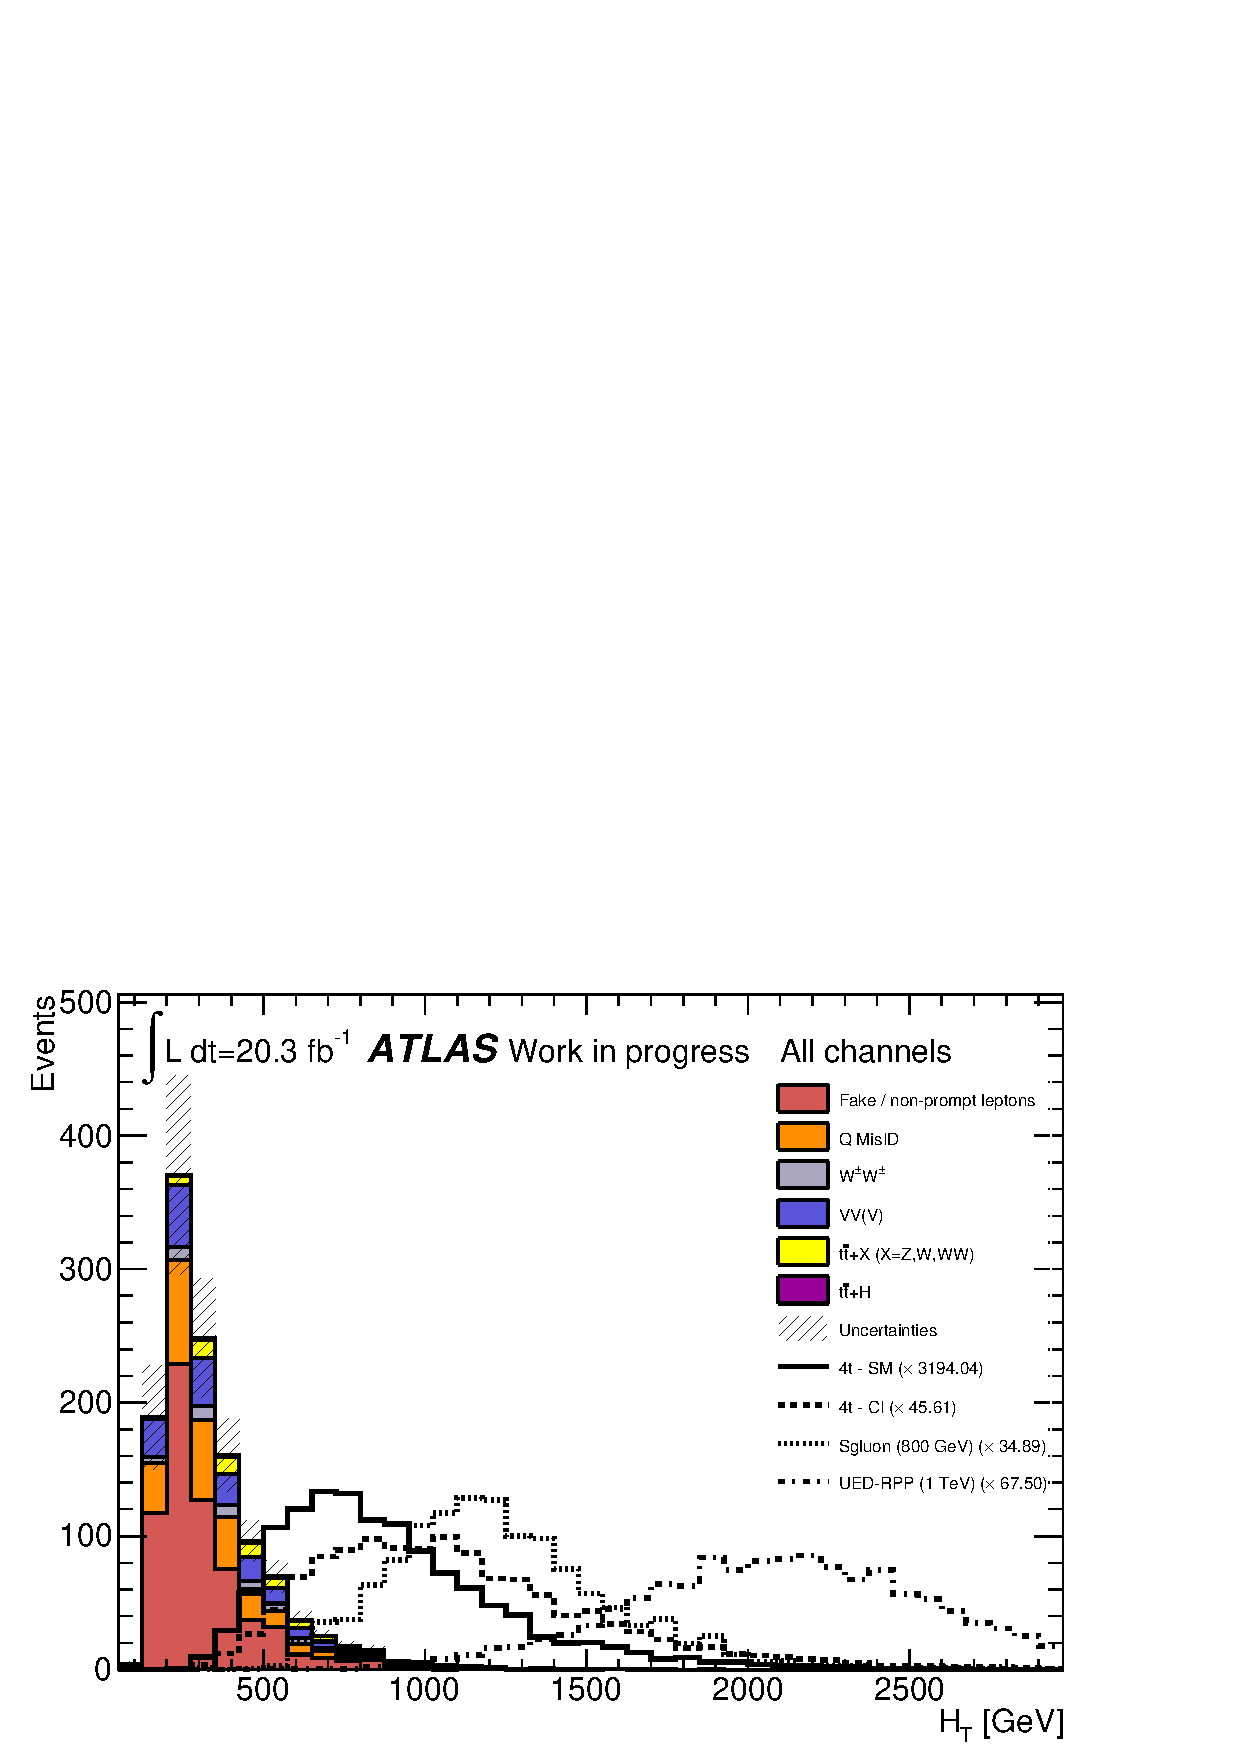
\includegraphics[width=0.48\linewidth]{figures/STD_END_SELECTION_alladded_HT_alladded.pdf}
%\includegraphics[width=0.45\linewidth]{Figures/Optimisations/Categorisation/Motivations/STD_END_SELECTION_alladded_MET_alladded.eps}
%\includegraphics[width=0.45\linewidth]{Figures/Optimisations/Categorisation/Motivations/STD_END_SELECTION_alladded_Nbjets_alladded.eps}
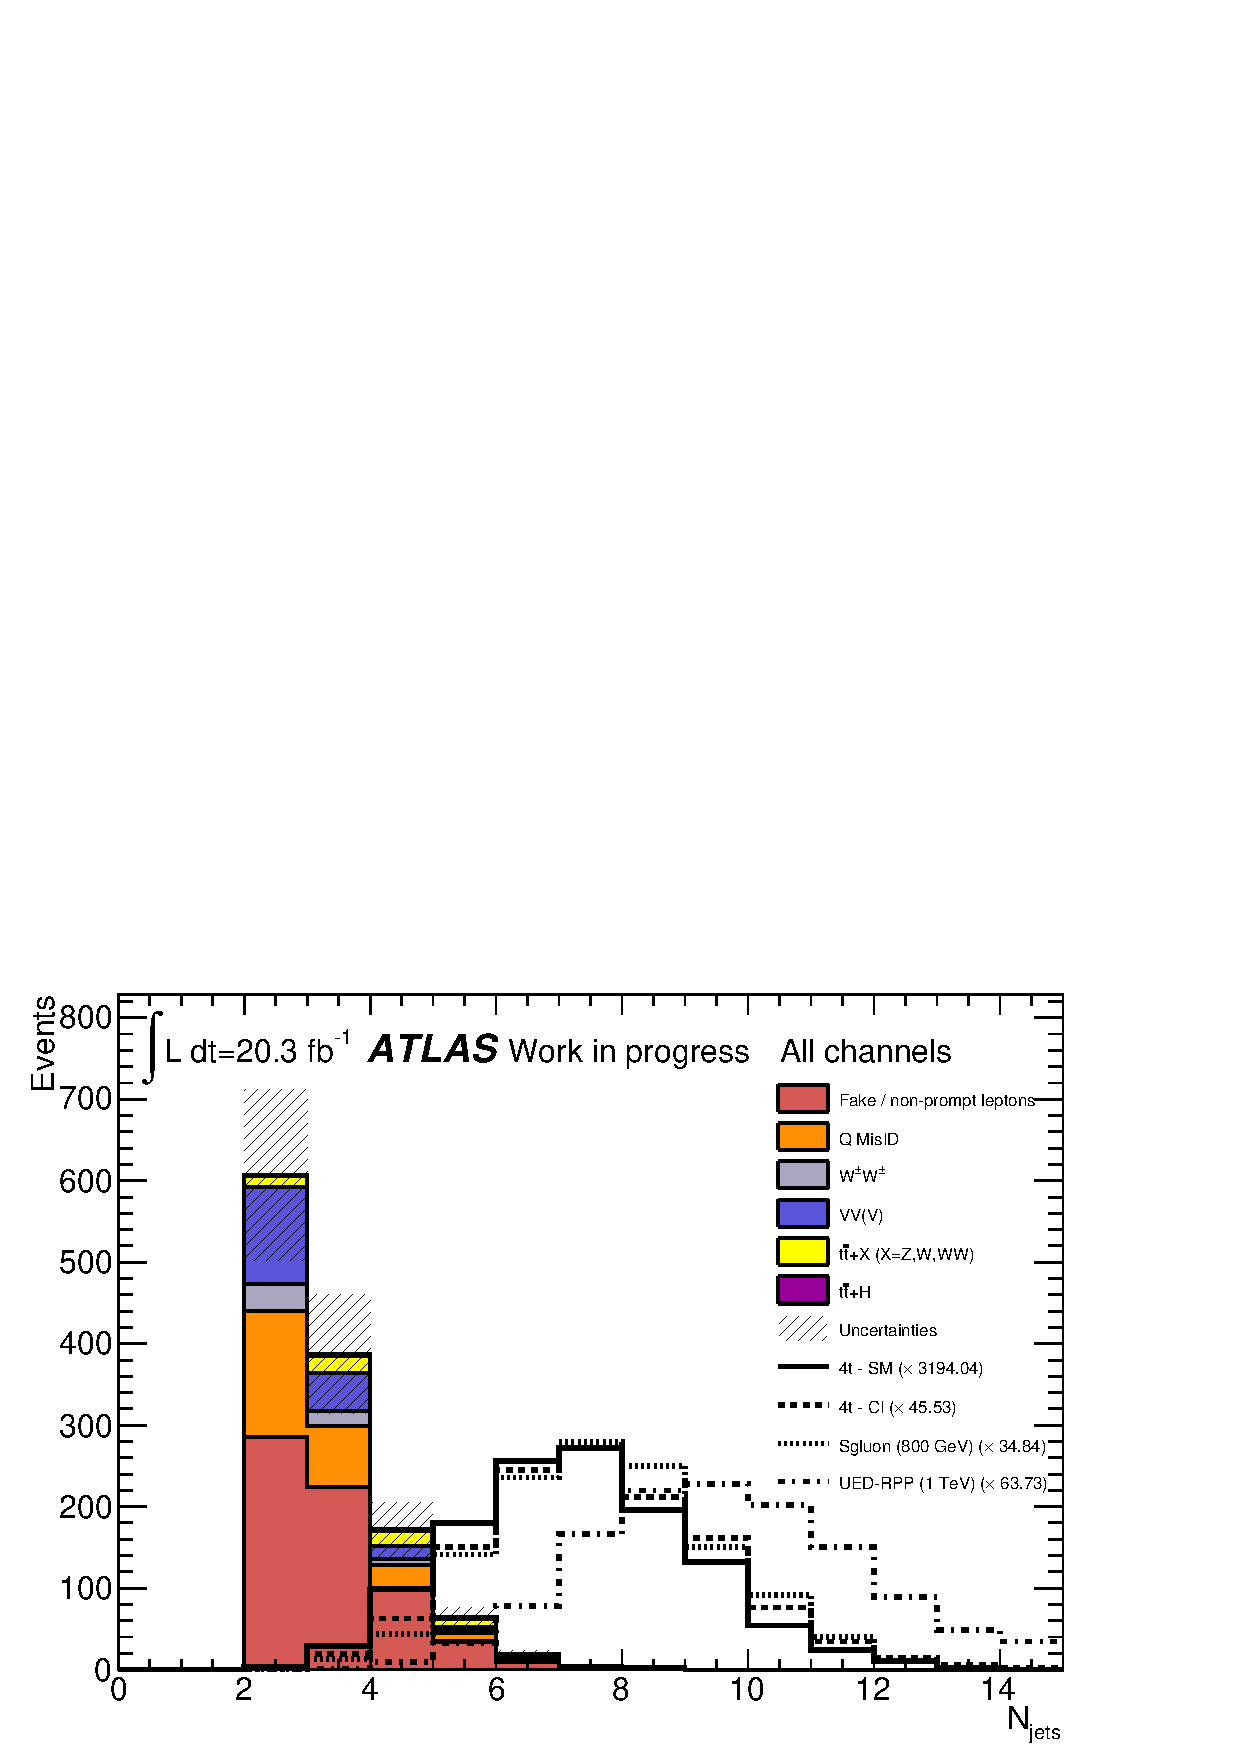
\includegraphics[width=0.48\linewidth]{figures/STD_END_SELECTION_alladded_Njets_alladded.pdf}
\end{center}
\vspace*{-0.5cm}
\caption{Distribution de l'impulsion transverse totale $H_T$ et du nombre de jets par \'ev\'enement pour les diff\'erents signaux \fourtop{} et pour le bruit de fond. Les canaux leptoniques sont ajout\'es.}
\label{fig:opt:cat:distrib_var_4tops}
\end{figure}

Une fois les coupures pr\'ec\'edentes appliqu\'ees, une cat\'egorisation des \'ev\'enements permettant de d\'efinir cinq r\'egions de signal est r\'ealis\'ee. Celles-ci sont pr\'esent\'ees dans la table~\ref{tab:allSR}. Les limites d'exclusion donn\'ees ci-dessous sont obtenues, pour tous les signaux, en combinant ces cinq cat\'egories.

\begin{table*}[!htb]
	\begin{center}
	\begin{tabular}{ c | c | c | c }
	\hline
	\multicolumn{3}{c|}{D\'efinition} & Nom \\
        \hline
	\multirow{2}{*}{$400~< H_T < 700~\GeV{}$}		& \multicolumn{2}{c|}{$N_b = 2$} &  SR4t0 \\
	\cline{2-4}
	 				& \multicolumn{2}{c|}{$N_b \geq 3$} &SR4t1 \\
	\hline
	\multirow{3}{*}{$H_T \geq 700~\GeV$} 			& \multirow{2}{*}{$N_b = 2$}  				& $40~< \hbox{\met} < 100~\GeV$ 		&  SR4t2 \\
	\cline{3-4}
											 &					 				& $\hbox{\met}\geq 100~\GeV$					&  SR4t3 \\
	\cline{2-4}
											&  \multicolumn{2}{c|}{$N_b \geq 3$} & SR4t4 \\
	\hline
\end{tabular}
\caption{D\'efinitions des r\'egions de signal.\label{tab:allSR}}
\end{center}
\end{table*} 

Les bruits de fond consid\'er\'es dans cette analyse sont de deux types :
\begin{maliste}
\item Bruits de fond physiques : il s'agit des processus du mod\`ele standard conduisant \`a la production de deux leptons de m\^eme charge ou de trois leptons. Les processus consid\'er\'es sont ceux dont les \'etats finaux sont $t\bar{t}W$, $t\bar{t}Z$, $t\bar{t}WW$, $WW$, $WZ$, $ZZ$, $t\bar{t}H$, $WH$, $ZH$, $WWW^*$, $ZWW^*$, $tWZ$ et $tH$.
\item Bruits de fond instrumentaux : il s'agit d'\'ev\'enements dans lesquels des objets sont soit mal identifi\'es soit mal reconstruits et qui de ce fait passent les coupures de s\'election. Ces \'ev\'enements sont de deux types. Le premier correspond \`a des \'ev\'enements dans lesquels un ou plusieurs jets sont reconstruits comme des leptons (ce bruit de fond sera d\'enomm\'e \english{fakes} par la suite). Le deuxi\`eme correspond \`a des \'ev\'enements avec deux leptons de charges oppos\'ees dans lesquels la charge de l'un d'entre eux est mal reconstruite (ce bruit de fond sera d\'enomm\'e \english{mis-id} par la suite).
\end{maliste}

Les bruits de fond physiques sont estim\'es gr\^ace \`a la simulation Monte Carlo. Les incertitudes syst\'ematiques consid\'er\'ees sont les incertitudes th\'eoriques sur les sections efficace de production, les incertitudes li\'ees aux radiations dans les \'etats initiaux et finaux, l'incertitude sur la luminosit\'e, les incertitudes sur les efficacit\'es d'identification et la r\'esolution des jets et des leptons et l'incertitude sur l'efficacit\'e d'identification des jets provenant de quarks $b$.

Les bruits de fond instrumentaux sont estim\'es sur les donn\'ees. Les incertitudes sur les taux de mauvaise identification des jets et de mauvaise reconstruction de la charge \'electrique ont \'et\'e estim\'es et pris en compte dans les calculs de limite d'exclusion.

\subsection{R\'esultats}
\label{sec:resultatsAnalyseFourTops}

Les nombres d'\'ev\'enements observ\'es et attendus pour les bruits de fond et le signal dans les cinq r\'egions de signal sont donn\'es dans la table~\ref{tab:allYields} et montr\'es sur la figure~\ref{fig:yieldsBkgSigPlusSignif} (les septs canaux leptoniques sont additionn\'es). 
Cette figure montre \'egalement les nombres d'\'ev\'enements dans des r\'egions de signal autres que celles d\'ecrites jusqu'ici (SRVLQx). 
Ces r\'egions ne sont pas consid\'er\'ees dans l'analyse pr\'esent\'ee dans ce document et ne sont donc pas d\'etaill\'ees. 
Les deux r\'egions qui contribuent le plus \`a l'acceptance pour la production d'\'ev\'enements \fourtop{} par interaction de contact et par le mod\`ele 2UED/RPP sont de loin les r\'egions SR4t3 et SR4t4. 
Le bruit de fond dominant est le processus $t\bar{t}W/Z$. 
Les deux autres fonds qui contribuent de mani\`ere significative sont les fonds \english{mis-id} et \english{fakes}. 
Le nombre d'\'ev\'enements nominal pr\'edit pour ce dernier est faible mais les incertitudes sont grandes (notamment l'incertitude statistique).
Les limites d'exclusion sont davantage d\'egrad\'ees par ces incertitudes que par les autres fonds dont le nombre d'\'ev\'enements nominal est plus grand mais l'incertitude plus faible.
Pour la production d'\'ev\'enements par le mod\`ele standard, ce sont aussi les r\'egions SR4t3 et SR4t4 qui fournissent le plus de signal mais, contrairement au cas des autres signaux, les autres r\'egions contribuent de mani\`ere non n\'egligeable.

Un bon accord entre la pr\'ediction sous l'hypoth\`ese de bruit de fond et l'observation est obtenu dans toutes les r\'egions, sauf dans SR4t3 et SR4t4 o\`u un exc\`es d'\'ev\'enements est pr\'esent dans les donn\'ees. 

\begin{comment}
\begin{table}[!htb]
  \begin{center}
  \hspace*{-1cm}
  \scalebox{0.9}{    \begin{tabular}{l c | c | c | c |c }
      \cline{2-6}\cline{2-6}
      & {\bf SR4t0} & {\bf SR4t1} & {\bf SR4t2} & {\bf SR4t3} & {\bf SR4t4} \\
      \cline{2-6}
      \multicolumn{6}{c}{\bf 2UED/RPP} \\
      \hline
      \multicolumn{1}{c|}{600~\GeV} & $7,7 \pm 1,3 $ & $5,9 \pm 1,1 $ & $81 \pm 4 $ & $321 \pm 9 $ & $588 \pm 11 $\\
      \multicolumn{1}{c|}{800~\GeV} & $0,08 \pm 0,04 $ & $0,12 \pm 0,05 $ & $6,9 \pm 0,4 $ & $38,7 \pm 0,9 $ & $60,9 \pm 1,0 $\\
      \multicolumn{1}{c|}{1000~\GeV} & $ ( 9 \pm 5) \cdot 10^{-3}  $ & $ ( 5 \pm 5) \cdot 10^{-4}  $ & $0,77 \pm 0,05 $ & $5,02 \pm 0,12 $ & $6,72 \pm 0,13 $\\
      \multicolumn{1}{c|}{1200~\GeV} & $< 1,9 \cdot 10^{-4}$ & $< 1,9 \cdot 10^{-4}$ & $ ( 74 \pm 5) \cdot 10^{-3}  $ & $0,648 \pm 0,014 $ & $0,689 \pm 0.013 $\\
      \hline
      \multicolumn{6}{c}{\bf Mod\`ele standard} \\
      \cline{2-6}
      & $ ( 42,8 \pm 2,1) \cdot 10^{-3}  $ & $ ( 38,8 \pm 2.0) \cdot 10^{-3}  $ & $ ( 25,8 \pm 1.7) \cdot 10^{-3}  $ & $ ( 58,3 \pm 2.7) \cdot 10^{-3}  $ & $ ( 105,7 \pm 3.4) \cdot 10^{-3}  $\\
      \cline{2-6}
      \multicolumn{6}{c}{\bf Interaction de contact ($C/\Lambda^2=-4\pi$~TeV$^{-2}$)} \\
      \cline{2-6}
      & $1,60 \pm 0,10 $                  & $1,26 \pm 0,09 $                  & $1,96 \pm 0,12 $                   & $5,26 \pm 0,20 $                    & $8,88 \pm 0,24 $  \\
      \cline{2-6}
      \multicolumn{6}{c}{\bf Bruits de fond} \\
      \hline

       \multicolumn{1}{c|}{$t\bar{t}t\bar{t}$}     & $0,04\pm 0,00 \pm\ 0,03$ & $0,04\pm 0,00 \pm\ 0,03$ & $0,03\pm 0,00 \pm\ 0,02$ & $0,06\pm 0,00 \pm\ 0,05$ & $0,10\pm 0,00 \pm\ 0,08$\\
       \multicolumn{1}{c|}{WZ/ZZ}                        & $0,88\pm 0,19 \pm\ 0,25$ & $0,07\pm 0,12 \pm\ 0,05$ & $0,30\pm 0,14 \pm\ 0,10$ & $0,02\pm 0,12 \pm\ 0,02$ & $0,00\pm 0,12 \pm\ 0,00$\\
       \multicolumn{1}{c|}{$W^{\pm}W^{\pm}$}      & $0,07\pm 0,02 \pm\ 0,02$ & $0,00\pm 0,01 \pm\ 0,00$ & $0,03\pm 0,01 \pm\ 0,02$ & $0,02\pm 0,01 \pm\ 0,02$ & $0,00\pm 0,01 \pm\ 0,00$\\
       \multicolumn{1}{c|}{$t\bar{t}W/Z$}           & $12,60\pm 0,28 \pm\ 4,86$ & $1,24\pm 0,09 \pm\ 0,49$ & $1,87\pm 0,09 \pm\ 0,73$ & $2,46\pm 0,11 \pm\ 0,98$ & $0,57\pm 0,05 \pm\ 0,23$\\
       \multicolumn{1}{c|}{$t\bar{t}WW$}          & $0,20\pm 0,01\pm\ 0,06$ & $0,02\pm 0,00\pm\ 0,01$ & $0,04\pm 0,00\pm\ 0,01$ & $0,09\pm 0,01\pm\ 0,03$ & $0,02\pm 0,00\pm\ 0,01$\\
       \multicolumn{1}{c|}{$t\bar{t}H$}              & $1,79\pm 0,09\pm\ 0,23$ & $0,26\pm 0,03\pm\ 0,05$ & $0,31\pm 0,04\pm\ 0,05$ & $0,44\pm 0,04\pm\ 0,06$ & $0,08\pm 0,02\pm\ 0,02$\\
       \multicolumn{1}{c|}{Triboson}                   & $0,00\pm 0,00\pm\ 0,00$ & $0,00\pm 0,00\pm\ 0,00$ & $0,00\pm 0,00\pm\ 0,00$ & $0,00\pm 0,00\pm\ 0,00$ & $0,00\pm 0,00\pm\ 0,00$\\
       \multicolumn{1}{c|}{VH}                             & $0,02\pm 0,03\pm\ 0,01$ & $0,00\pm 0,08\pm\ 0,00$ & $0,00\pm 0,08\pm\ 0,00$ & $0,00\pm 0,08\pm\ 0,00$ & $0,00\pm 0,08\pm\ 0,00$\\
       \multicolumn{1}{c|}{tX}                               & $0,49\pm 0,02\pm\ 0,07$ & $0,04\pm 0,01\pm\ 0,01$ & $0,09\pm 0,01\pm\ 0,01$ & $0,08\pm 0,01\pm\ 0,01$ & $0,02\pm 0,00\pm\ 0,00$\\
       \multicolumn{1}{c|}{Fakes}                      & $8,61\pm 2,34\pm\ 5,02$ & $1,17\pm 0,82\pm\ 0,68$ & $1,03\pm 0,97\pm\ 0,60$ & $0,00\pm 1,02\pm\ 0,00$ & $0,04\pm 0,83\pm\ 0,02$\\
       \multicolumn{1}{c|}{Mis-Id}                   & $15,07\pm 0,55\pm\ 3,52$ & $0,74\pm 0,11\pm\ 0,18$ & $1,17\pm 0,16\pm\ 0,38$ & $1,09\pm 0,14\pm\ 0,34$ & $0,30\pm 0,09\pm\ 0,10$\\
\hdashline
       \multicolumn{1}{c|}{Total}               & $39,76 \pm 2,43\pm\ 7,26 $ & $3,57 \pm 0,85\pm\ 0,84 $ & $4,86 \pm 1,00\pm\ 1,01 $ & $4,25 \pm 1,05\pm\ 1,07 $ & $1,12 \pm 0,85\pm\ 0,28 $\\

      \hline
       \multicolumn{6}{c}{\bf Observ\'e} \\ \cline{2-6}
                                      & 54 & 6 & 6 & 12 & 6 \\ \cline{2-6}
    \end{tabular}}
    \caption{Nombre d'\'ev\'enements attendu pour les bruits de fond et les signaux recherchés et nombre d'événement observé dans les diff\'erentes r\'egions de signal. Les incertitudes sur les nombres d'\'ev\'enements pour les signaux sont les incertitudes statistiques. Pour les bruits de fond, les premi\`eres et deuxi\`emes incertitudes sont respectivement les incertitudes statistiques et syst\'ematiques (ces derni\`eres sont donn\'ees par l'\'ecart-type de la distribution marginale du nombre d'\'ev\'enements). Pour la production par interaction de contact, les valeurs ont \'et\'e obtenus avec $C/\Lambda^2=-4\pi$~TeV$^{-2}$.\label{tab:allYields}}
  \end{center}
\end{table}
\end{comment}

\begin{table}[!htb]
  \begin{center}
%  \hspace*{-1.cm}
  \scalebox{0.75}{    \begin{tabular}{|l | c | c | c | c |c | }
      \cline{2-6}%\cline{2-6}
       \multicolumn{1}{c|}{ } & {\bf SR4t0} & {\bf SR4t1} & {\bf SR4t2} & {\bf SR4t3} & {\bf SR4t4} \\ \cline{2-6}
       \multicolumn{6}{c}{\bf Signaux} \\
      \hline
      $m_{KK}=600$~\GeV & $7,7 \pm 1,3 $ & $5,9 \pm 1,1 $ & $81 \pm 4 $ & $321 \pm 9 $ & $588 \pm 11 $\\
      $m_{KK}=800$~\GeV & $0,08 \pm 0,04 $ & $0,12 \pm 0,05 $ & $6,9 \pm 0,4 $ & $38,7 \pm 0,9 $ & $60,9 \pm 1,0 $\\
      $m_{KK}=1000$~\GeV & $ ( 9 \pm 5) \cdot 10^{-3}  $ & $ ( 5 \pm 5) \cdot 10^{-4}  $ & $0,77 \pm 0,05 $ & $5,02 \pm 0,12 $ & $6,72 \pm 0,13 $\\
      $m_{KK}=1200$~\GeV & $< 1,9 \cdot 10^{-4}$ & $< 1,9 \cdot 10^{-4}$ & $ ( 74 \pm 5) \cdot 10^{-3}  $ & $0,648 \pm 0,014 $ & $0,689 \pm 0.013 $\\
\hline
 Mod\`ele standard   & $ ( 42,8 \pm 2,1) \cdot 10^{-3}  $ & $ ( 38,8 \pm 2.0) \cdot 10^{-3}  $ & $ ( 25,8 \pm 1.7) \cdot 10^{-3}  $ & $ ( 58,3 \pm 2.7) \cdot 10^{-3}  $ & $ ( 105,7 \pm 3.4) \cdot 10^{-3}  $\\
      \hline
      Interaction contact & $1,60 \pm 0,10 $                  & $1,26 \pm 0,09 $                  & $1,96 \pm 0,12 $                   & $5,26 \pm 0,20 $                    & $8,88 \pm 0,24 $  \\
      \hline
      \multicolumn{6}{c}{\bf Bruits de fond} \\
      \hline

       $t\bar{t}W/Z$            & $12.6 \pm 0.3 \pm 5.4$       & $1.24 \pm 0.09\pm 0.53$& $1.87 \pm 0.09\pm 0.80$ & $2.46 \pm 0.11\pm 1.06$ & $0.57\pm 0.05 \pm 0.25$ \\
      $t\bar{t}H$                & $1.8 \pm 0.1 \pm 0.2$           & $ 0.26 \pm 0.03 \pm 0.05$&  $0.31 \pm 0.04\pm 0.05$ & $0.44\pm 0.04\pm 0.06$ & $0.08\pm 0.02\pm 0.02$\\
       Dibosons                    & $0.95 \pm 0.19\pm 0.25$       & $0.07 \pm 0.12 \pm 0.05$ & $0.33\pm 0.14\pm 0.10$ & $0.04\pm 0.12\pm 0.03$ & $0.00\pm 0.12\pm 0.00$ \\
       Fake/Non-prompt   & $8.61 \pm 2.34 \pm 5.02$ & $1.17 \pm 0.82 \pm 0.68$&  $1.03\pm 0.97 \pm 0.60$ & $0.00\pm 1.02 \pm 0.28$ & $0.04\pm 0.83 \pm 0.24$\\    
       Q mis-Id                    & $15.1 \pm 0.6 \pm 3.5$           & $0.74 \pm 0.11 \pm 0.18$&  $1.17\pm 0.16 \pm 0.38$ & $1.09\pm 0.14 \pm 0.34$ & $0.30\pm 0.09 \pm 0.10$\\  
      Autres                        & $0.75 \pm 0.04 \pm 0.10$      & $0.10 \pm 0.08 \pm 0.03$ &  $0.16\pm 0.08\pm 0.02$ & $0.23\pm 0.08\pm 0.05$ & $0.14\pm 0.08\pm 0.08$\\        
\hdashline
       Total               & $40.0 \pm 2.4 \pm 7.3 $ & $3.6 \pm 0.9 \pm 0.8$ & $4.9 \pm 1.0 \pm 1.0 $ & $4.3 \pm 1.1 \pm 1.1 $ & $1.1 \pm 0.9 \pm 0.4 $\\

      \hline
       \multicolumn{6}{c}{\bf Observ\'e} \\ \cline{2-6}
       \multicolumn{1}{c|}{}                         & 54 & 6 & 6 & 12 & 6 \\ \cline{2-6}
    \end{tabular}}
    \caption{Nombre d'\'ev\'enements attendu pour les signaux recherchés et les bruits de fond et nombre d'événements observés dans les diff\'erentes r\'egions de signal. Les incertitudes sur les nombres d'\'ev\'enements pour les signaux sont les incertitudes statistiques. Pour les bruits de fond, les premi\`eres et deuxi\`emes incertitudes sont respectivement les incertitudes statistiques et syst\'ematiques (ces derni\`eres sont donn\'ees par l'\'ecart-type de la distribution marginale du nombre d'\'ev\'enements). Pour la production par interaction de contact, les nombres donn\'es ont \'et\'e obtenus avec $C/\Lambda^2=-4\pi$~TeV$^{-2}$.\label{tab:allYields}}
  \end{center}
\end{table}

\begin{figure}[!htb]
\begin{center}
\vspace*{-0.5cm}
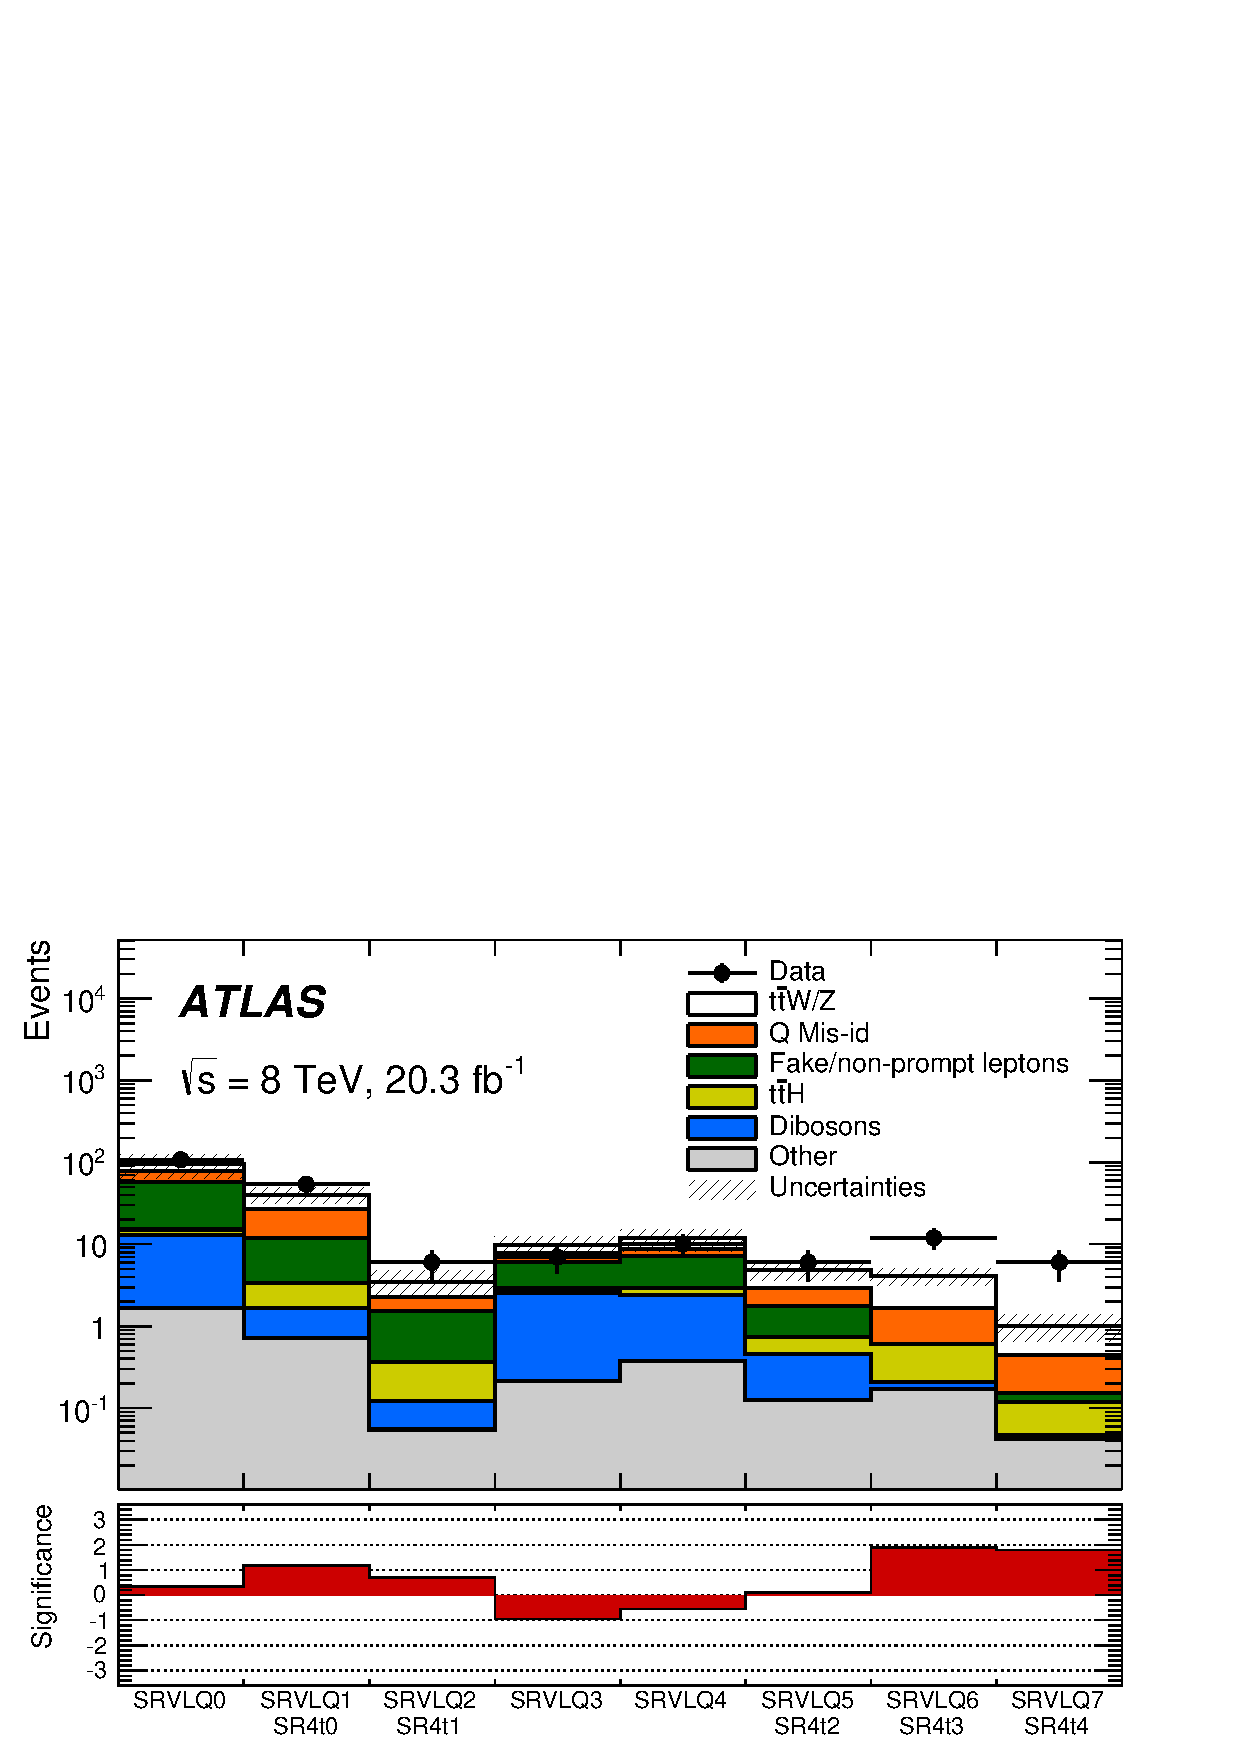
\includegraphics[width=0.65\linewidth]{figures/paperSameSign/ExpectedBackgroundObeservedCategories.pdf}
\end{center}
\vspace*{-0.3cm}
\caption{Nombre d'\'ev\'enements de bruit de fond attendus et observ\'es (en haut) et significance de l'observation (en bas) dans les diff\'erentes r\'egions de signal.}
\label{fig:yieldsBkgSigPlusSignif}
\end{figure}

La significance de l'exc\`es est quantifi\'ee en calculant la \pval~de l'observation sous l'hypoth\`ese de bruit de fond, par la suite not\'ee $p$. 
Celle-ci est dans une tr\`es bonne approximation \'egale \`a $1-\CLb$. 
Elle est traduite en significance par l'expression
\[Z=\Phi^{-1}\left(1-p\right)\]
o\`u $\Phi$ est la fonction de r\'epartition de la distribution normale centr\'ee r\'eduite. 
La significance dans SR4t3 et SR4t4 est tr\`es l\'eg\`erement inf\'erieure \`a $2\sigma$, comme le montre le graphique du bas sur la figure~\ref{fig:yieldsBkgSigPlusSignif}. 
Il s'agit donc d'un exc\`es mod\'er\'e.
Les donn\'ees de cette analyse ont par cons\'equent \'et\'e utilis\'ees pour contraindre les mod\`eles de nouvelle physique consid\'er\'es. 

Les limites d'exclusion sont calcul\'ees avec la m\'ethode hybride fr\'equentiste-bay\'esienne d\'ecrite dans les chapitres~\ref{chap:interpretationStatLimit} et \ref{chap:OTHandTIFOSI}. 
Les cinq r\'egions de signal sont combin\'ees (chacune d'elle correspond \`a un canal $c$ dans l'\'equation~\ref{eq:fullLhoodOTH}). 
%Le programme utilis\'e pour calculer les limites d'exclusion officielles est \mclimit. 
Les distributions \prior~pour les incertitudes statistiques sont gaussiennes et l'interpolation et extrapolation nomm\'ee \text{"}\mclimit\text{"} dans la section~\ref{sec:OTHTreatmentSystUncerts} a \'et\'e utilis\'ee. 
Toutes les limites pr\'esent\'ees dans la suite ont \'et\'e calcul\'ees avec le programmes \mclimit{} et \opthylic. Un excellent accord a \'et\'e trouv\'e \`a chaque fois.

Les limites d'exclusion \`a $95\%$~CL sur les sections efficaces de production d'\'ev\'enements \fourtop{} par interaction de contact et par le mod\`ele standard sont montr\'ees dans la table \ref{tab:limitsExpObsSMCI}. Comme nous l'avons dit dans la section~\ref{sec:interactionContact}, l'\'etablissement d'une limite d'exclusion sur la section efficace de production d'\'ev\'enements \fourtop{} par interaction de contact permet d'exclure certaines r\'egions du plan $\left(C,\Lambda\right)$. Les limites d'exclusion dans ce plan sont montr\'ees sur la figure~\ref{fig:Limit4tCIRPP_20fbObs}(a).

\begin{table}[!htb]
  \begin{center}
    \begin{tabular}{l|c|c | c}
      \hline
      & attendu \`a $1\sigma$ & attendu m\'ediane & observ\'ee\\
      \hline
      Mod\`ele standard   & $\left[18-41\right]$ & $27$ & $70$ \\
      Interaction contact & $\left[16-34\right]$ & $22$  & $61$ \\
      \hline      
    \end{tabular}
    \caption{Limites attendues et observ\'ees sur les sections efficaces de production d'\'ev\'enements \fourtop{} par interaction de contact et par le mod\`ele standard (en fb).}\label{tab:limitsExpObsSMCI}
  \end{center}
\end{table}

\begin{figure}
\centering
\vspace*{-0.5cm}
%\includegraphics[width=0.54\linewidth]{figures/Limit4tCI_20fbObs.pdf}
\includegraphics[width=0.49\linewidth]{figures/paperSameSign/Limit4tCI_20fbObs.pdf}
%\subfloat[toto]{\includegraphics[scale=0.5]{figures/paperSameSign/Limit4tCI_20fbObs.pdf}}
%\includegraphics[width=0.57\linewidth]{figures/RPP_observed_1D11.pdf}
\includegraphics[width=0.49\linewidth]{figures/paperSameSign/RPP_observed_1D11.pdf}
%\subfloat[tata]{\includegraphics[scale=0.5]{figures/paperSameSign/RPP_observed_1D11.pdf}}
%\vspace*{-0.5cm}
\put(-325,-10){$(a)$}
\put(-100,-10){$(b)$}
\caption{Limites d'exclusion attendues et observ\'ee \`a 95\% CL sur la constante $C$ en fonction de l'\'echelle en \'energie $\Lambda$ pour la production d\'ev\'enements \fourtop{} par interaction de contact (\`a gauche) et sur la section efficace de production d'\'ev\'enements \fourtop{} par le mod\`ele 2UED/RPP en fonction de $m_{KK}$ (\`a droite). \label{fig:Limit4tCIRPP_20fbObs}}
\end{figure}

Les limites d'exclusion attendues et observ\'ees en fonction de $m_{KK}$ pour le signal 2UED/RPP sont montr\'ees sur la figure~\ref{fig:Limit4tCIRPP_20fbObs}(b). La section efficace th\'eorique est \'egalement montr\'ee. La limite inf\'erieure attendue m\'ediane (observ\'ee) sur $m_{KK}$ est de 1,05~\TeV{} (0,96~\TeV). Ces limites sont, comme nous l'avons vu dans la section~\ref{sec:modele2UED/RPP}, d\'etermin\'ees en faisant l'hypoth\`ese que les rayons $R_4$ et $R_5$ sont \'egaux ($\xi=1$). Au premier ordre, la section efficace de production ainsi que la cin\'ematique des \'ev\'enements provenant de l'\'etage $\left(1,1\right)$ ne d\'epend que de 
\[\sqrt{\frac{1}{R_4^2}+\frac{1}{R_5^2}}=m_{KK}\sqrt{1+\xi^2}\]

Les limites obtenues sur $m_{KK}$ pour $\xi=1$ peuvent donc \^etre utilis\'ees pour mettre des limites sur $m_{KK}$ pour des valeurs diff\'erentes de $\xi$. La figure~\ref{fig:RPP_observed_2D} montre les limites d'exclusion attendues et observ\'ees dans le plan $\left(\xi,m_{KK}\right)$. Les contraintes cosmologiques sont \'egalement montr\'ees. 

\begin{figure}[!htb]
\begin{center}
\vspace*{-1cm}
%\includegraphics[scale=0.8]{figures/RPP_observed_2D.pdf}
\includegraphics[scale=0.5]{figures/paperSameSign/RPP_observed_2D_snapshotfrompaper.pdf}
\end{center}
\vspace*{-2.5cm}
\caption{Limites d'exclusion attendue et observ\'ee \`a 95\% CL sur $\xi$ en fonction de $m_{KK}$ pour le mod\`ele 2UED/RPP. Les contraintes cosmologiques sont \'egalement montr\'ees.}
\label{fig:RPP_observed_2D}
\end{figure}
%\clearpage

La figure~\ref{fig:Limit4tCIRPP_20fbObs} montre que, lorsque toutes les r\'egions de signal sont combin\'ees, la significance de l'observation est sup\'erieure \`a 2$\sigma$. 
Les distributions du test sous l'hypoth\`ese de bruit de fond pour l'interaction de contact et pour le signal 2UED/RPP avec $m_{KK}=1000~$GeV sont montr\'ees sur la figure~\ref{fig:significanceCIRPPWithOTH}. 
Nous en d\'eduisons que la significance est \'egale \`a environ 2,4 pour la production d'\'ev\'enements \fourtop{} par interaction de contact et environ 2,5 pour la production par le mod\`ele 2UED/RPP avec $m_{KK}=1000~$GeV.

\begin{figure}[!htb]
\begin{center}
\includegraphics[width=0.43\linewidth]{macros/significanceContactInteractionMcLimitNormal.pdf}
\includegraphics[width=0.43\linewidth]{macros/significance2UEDRPPMkk1000McLimitNormal.pdf}
\end{center}
\vspace*{-0.7cm}
\caption{Distribution du test statistique $\qmu$ sous l'hypoth\`ese de bruit de fond pour la production d'\'ev\'enements \fourtop{} par interaction de contact (\`a gauche) et par le mod\`ele 2UED/RPP avec $m_{KK}=1000$~GeV. La valeur observ\'ee $\qmuobs$ est repr\'esent\'ee par la ligne verticale. La \pval~$p$ et la significance $Z$ de l'observation sont \'egalement donn\'ees.\label{fig:significanceCIRPPWithOTH}}
\end{figure}

Ces valeurs de significance montrent que la diff\'erence entre l'observation et la pr\'ediction commence \`a \^etre significative lorsque toutes les r\'egions de signal sont combin\'ees. 
Plusieurs v\'erifications ont \'et\'e effectu\'ees afin de v\'erifier que cette diff\'erence ne provient pas d'une mauvaise estimation des bruits de fond. 
Pour les fonds $t\bar{t}W/Z$, diff\'erents g\'en\'erateurs et diff\'erents r\'eglages de ces g\'en\'erateurs ont \'et\'e utilis\'es. 
Pour les fonds intrumentaux, il a \'et\'e v\'erifi\'e que les leptons se trouvant dans les r\'egions SR4t3 et SR4t4 ont des propri\'et\'es similaires \`a celles attendues pour des vrais leptons. 
De plus, ces fonds ont \'et\'e estim\'es avec la simulation uniquement. 
Dans tous les cas, les nombres d'\'ev\'enements obtenus dans les diff\'erentes r\'egions de signal sont compatibles avec ceux issus de l'estimation nominale.

% La figure~\ref{} montre les distributions des variables $H_T$ et du nombre de jets

\begin{comment}
\blabla contribution des diff\'erentes categories a la sensibilite\\
\\
\blabla bkg pour 2lep et 3leps\\
\\
\blabla exces -> commenter (mettre plot pValue)


\subsection{V\'erification avec \opthylic}

Toutes les limites d'exclusion pour les signaux consid\'er\'es dans ce chapitre ont \'et\'e v\'erifi\'ees avec \opthylic. Un bon accord entre \mclimit{} et \opthylic~a \'et\'e observ\'e. La figure~\ref{fig:ExclusionPlot_RPPFullStat_OTHVsBayesian} montre les r\'esultats obtenus avec ces deux programmes dans le cas du signal 2UED/RPP.

\begin{figure}[!htb]
\begin{center}
\includegraphics[width=0.54\linewidth]{macros/ExclusionPlot_RPPFullStat_McLimitVsOTH.pdf}
\end{center}
\caption{Comparaison des limites observ\'ees et attendues calcul\'ees avec \mclimit~et \opthylic~pour le signal 2UED/RPP.}
\label{fig:ExclusionPlot_RPPFullStat_OTHVsBayesian}
\end{figure}

Les significances d'observation ont \'egalement \'et\'e calcul\'ees avec \opthylic. La figure~\ref{fig:significanceCIRPPWithOTH} montre par exemple la distribution du test statistique sous l'hypoth\`ese de bruit de fond ainsi que sa valeur observ\'ee pour la production d'\'ev\'enements par interaction de contact et par le mod\`ele 2UED/RPP. La valeur de $\mu$ utilis\'ee pour calculer le test $\qmu$ est $\mu=1$. Les valeurs de significance sont en très bon accord avec celles trouvées par \mclimit{} et confortent ainsi les r\'esultats obtenus.

\begin{figure}[!htb]
\begin{center}
\includegraphics[width=0.43\linewidth]{macros/significanceContactInteractionMcLimitNormal.pdf}
\includegraphics[width=0.43\linewidth]{macros/significance2UEDRPPMkk1000McLimitNormal.pdf}
\end{center}
\caption{Distribution du test statistique $\qmu$ sous l'hypoth\`ese de bruit de fond pour la production d'\'ev\'enements \fourtop{} par interaction de contact (\`a gauche) et par le mod\`ele 2UED/RPP avec $m_{KK}=1000$~GeV. La valeur observ\'ee $\qmuobs$ est repr\'esent\'ee par la ligne verticale. La \pval~$p$ et la significance $Z$ de l'observation sont \'egalement donn\'ees.\label{fig:significanceCIRPPWithOTH}}
\end{figure}

\end{comment}

\subsection{Variation d'interpr\'etation}

En plus des v\'erifications d\'ecrites ci-dessus, d'autres \'etudes ont \'et\'e r\'ealis\'ees sur l'interpr\'etation statistique des donn\'ees.
Comme nous l'avons vu dans les chapitre~\ref{chap:interpretationStatLimit} et \ref{chap:OTHandTIFOSI}, toute interpr\'etation statistique contient une part d'arbitraire li\'ee aux choix qui sont faits pour r\'ealiser les calculs (que ce soit les calculs de limite ou de significance). 
Ces choix sont de deux types. Premi\`erement, il y a le choix de l'approche statistique. 
Les r\'esultats publi\'es pr\'esent\'es ci-dessus ont \'et\'e obtenus avec une approche hybride et il est int\'eressant de les comparer \`a ceux obtenus par une approche fr\'equentiste et bay\'esienne. 
Deuxi\`emement, il y a les choix relatifs au traitement des incertitudes statistiques et syst\'ematiques. 
Ces derniers doivent \^etre fait quelque soit l'approche statistique utilis\'ee.
Les sections suivantes pr\'esentent les r\'esultats obtenus en faisant varier ces choix. 
%La robustesse des r\'esultats publi\'es . 

\subsubsection{Interpr\'etation hybride vari\'ee}
\label{sec:variationInterpretationFourTopHybride}

Les limites d'exclusion et significances d'observation ont \'et\'e calcul\'ees avec \opthylic{} en faisant varier l'interpolation et extrapolation des incertitudes syst\'ematiques et les distributions \prior{} pour les incertitudes statistiques. La figure~\ref{fig:interpretationHybrideVariee} montre les limites pour les mod\`eles d'interaction de contact et 2UED/RPP avec $m_{KK}=1000~$GeV obtenues avec la configuration standard pr\'esent\'ee pr\'ec\'edemment et celles obtenues avec une interpolation polynomiale, une extrapolation exponentielle et une distribution \prior{} gamma donn\'ee par la formule~\ref{eq:gammaPriorsInOTH} (une distribution \prior{} $\pi\left(y\right)\propto 1/y$ est utilis\'ee). D'autres comparaisons ont \'et\'e effectu\'ees en changeant d'interpolation/extrapolation et en prenant des distributions \prior{} log-normales. 
Les limites obtenues sont similaires \`a celles obtenues avec la distribution gamma.

\vspace*{-0.5cm}
\begin{center}
\begin{figure}[!htb]
\includegraphics[width=0.45\textwidth]{macros/ExclusionPlot_RPPFullStat_McLimitVsOTHpolyexpo_gammahyper.pdf}
\includegraphics[width=.48\textwidth]{macros/CVsLambdaForContactInteractionMcLimitVsOTHpolyexpogammahyper.pdf}
\caption{Limites observ\'ees et attendues \`a $95\%$ CL pour le mod\`ele 2UED/RPP avec $m_{KK}=1000~$GeV (\`a gauche) et le mod\`ele d'interaction de contact (\`a droite) obtenue avec diff\'erents sch\'emas d'interpolation et extrapolation pour les incertitudes syst\'ematiques et diff\'erentes distributions \prior{} pour les incertitudes statistiques. Les r\'esultats pour l'interpolation et extrapolation nomm\'ee \text{"}\mclimit\text{"} et des distributions \prior{} normales sont montr\'es en vert, jaune et noir et ceux pour l'interpolation polynomiale, l'extrapolation exponentielle et des distributions \prior{} gammas sont montr\'es en gris. \label{fig:interpretationHybrideVariee}}
\end{figure}
\end{center}
\vspace*{-1cm}
Les diff\'erences entre la configuration standard et la configuration vari\'ee sont essentiellement dues au changement dans les distributions \prior{}. Le passage de distributions normales aux distributions gammas (ou log-normales) se traduit par un diminution de la valeur moyenne du nombre d'\'ev\'enements (ceci est vrai sous l'hypoth\`ese de bruit de fond et sous l'hypoth\`ese signal plus bruit de fond). 
La distribution du test est par cons\'equent d\'ecal\'ee vers les grandes valeurs.
De plus, elle est davantage asym\'etrique du fait de l'asym\'etrie de la distribution gamma (ou log-normale) lorsque son esp\'erance est faible. 
Ceci a pour effet de r\'eduire l\'eg\`erement les limites attendues. 
Les limites observ\'ees sont quant \`a elles plus grandes avec des distributions gammas. En effet, l'exc\`es est tel que \CLb{} est tr\`es proche de 1 quelque soient les distributions \prior. Il faut donc un $\mu$ plus grand avec les distributions gammas qu'avec les distributions normales pour atteindre $\CLsb=0,05$. 

Les diff\'erences que nous venons de d\'ecrire se traduisent \'egalement par des diff\'erences dans la significance de l'exc\`es. L'utilisation de distributions gamma (ou log-normale) fait passer la significance de 2,4 \`a 2,7 dans le cas de la production par interaction de contact et de 2,5 \`a 2,8 pour la production par le mod\`ele 2UED/RPP avec $m_{KK}=1000~$GeV. 

Ces \'etudes montrent qu'un changement d'interpr\'etation hybride conduit \`a des variations de 6\% \`a 12\% dans les limites d'exclusion et d'environ 12\% dans les significances.

\subsubsection{Interpr\'etation bay\'esienne}
\label{sec:variationInterpretationFourTopBayesian}

Les limites d'exclusion pour tous les signaux ont \'egalement \'et\'e calcul\'ees par l'approche bay\'esienne avec l'outil \tifosi~(voir section~\ref{sec:tifosi}). Pour tous les r\'esultats pr\'esent\'es ci-dessous, une distribution \prior~uniforme sur le param\`etre d'int\'er\^et $\mu$ a \'et\'e utilis\'ee. Les distributions \prior~pour les incertitudes statistique sont gaussiennes. L'interpolation et l'extrapolation utilis\'ees par le programme \mclimit{} n'\'etant pas disponible dans \tifosi, nous avons choisi l'interpolation polynomiale et l'extrapolation exponentielle d\'ecrites dans le chapitre~\ref{chap:OTHandTIFOSI}. Le niveau de cr\'edibilit\'e des intervalles bay\'esiens est choisi \'egal au niveau de confiance des intervalles hybrides, soit 95\% (rappelons que, dans le cas o\`u un seul canal est consid\'er\'e avec un signal parfaitement connu, l'utilisation d'une m\^eme valeur pour les deux niveaux conduit \`a la m\^eme inf\'erence sur $\mu$).

%Les diff\'erences entre les intervalles hybride et bay\'esien proviennent donc de la combinaison des canaux et de la pr\'esence d'incertitudes sur le nombre d'\'ev\'enement de signal attendu.

Les limites bay\'esienne et hybride (calcul\'ees avec \opthylic) pour les diff\'erents signaux sont donn\'ees dans la table~\ref{tab:comparaisonLimitesHybrideBayesienne}. 
\vspace*{0.5cm}
\begin{table}[!htb]
  \begin{center}
    \begin{tabular}{|c|c|c|c|c|}
      \hline
      \multirow{2}{*}{Signal}                  &  \multicolumn{2}{c|}{Limite attendue}       &  \multicolumn{2}{c|}{Limite observ\'ee}     \\ \cline{2-5}
                                                                    &  hybride              & bay\'esienne           &   hybride     &   bay\'esienne             \\ \hline
      2UED/RPP $m_{KK}=600$ GeV   &   8,67        &    6,98                &      23,0        &    21,8                     \\ \hline
      2UED/RPP $m_{KK}=800$ GeV   &    7,38       &     6,03               &     19,3         &    19,0                     \\ \hline  
      2UED/RPP $m_{KK}=1000$ GeV  &   6,62        &     5,62              &   17,5           &    16,7                  \\ \hline  
      2UED/RPP $m_{KK}=1200$ GeV  &    6,24          &     5,17           &    16,7          &     16,0                    \\ \hline  
      Interaction contact                       &     22,4       &      19,0                             &      61,2         &    66,3                        \\ \hline  
      Mod\`ele standard                        &     26,6     &         21,0                     &         70,1      &     66,7                       \\ \hline  
    \end{tabular}
    \caption{Limites d'exclusion sur la section efficace de production (en fb) pour les diff\'erents signaux consid\'er\'es dans cette analyse. Les limites hybrides (bay\'esiennes) sont calcul\'ees avec le programme \opthylic~\`a 95\% CL (\tifosi~\`a 95\% CI). Les limites bay\'esiennes sont calcul\'ees avec une distribution \prior~uniforme sur le param\`etre d'int\'er\^et. Les limites attendues sont les limites m\'edianes sous l'hypoth\`ese du bruit de fond dans le cas hybride et les limites calcul\'ees avec un échantillon \english{asimov} dans le cas bay\'esien. Pour la production par interaction de contact, les nombres d'\'ev\'enements ont \'et\'e obtenus avec $C/\Lambda^2=-4\pi$~TeV$^{-2}$}\label{tab:comparaisonLimitesHybrideBayesienne}
  \end{center}
\end{table}
\clearpage
Les limites attendues dans le cas bay\'esien sont calcul\'ees avec un \'echantillon \english{asimov}, c'est-\`a-dire, en utilisant les notations des chapitres~\ref{chap:interpretationStatLimit} et \ref{chap:OTHandTIFOSI}, avec
\[\nobsc=\sum\limits_i \bci\]
pour tous les canaux $c$. Les limites attendues bay\'esiennes sont plus faibles que les limites attendues hybrides de 15\% \`a 21\% en fonction du signal. 
Pour tous les signaux, les limites attendues bay\'esiennes se trouvent dans l'intervalle de confiance \`a $\pm 1\sigma$ obtenue dans le cas hybride. 
Les limites observ\'ees sont compatibles \`a 10\% pr\`es.



La figure \ref{fig:ExclusionPlot_RPPFullStatAndCI_OTHVsBayesian} montre les limites hybrides et bayésiennes observ\'ees et attendues pour le signal 2UED/RPP en fonction de $m_{KK}$ (\`a gauche) et pour l'interaction de contact (\`a droite). Les limites observ\'ees et attendues sur $m_{KK}$ sont sensiblement les m\^emes dans les deux cas (elles sont augment\'ees avec le calcul bay\'esien d'environ 16~GeV et 3,5~GeV respectivement). Les r\'egions exclues dans le plan $\left(C,\Lambda\right)$ changent elles-aussi relativement peu. 

\begin{figure}[!htb]
\begin{center}
\includegraphics[width=0.45\linewidth]{macros/ExclusionPlot_RPPFullStat_OTHVsBayesian.pdf}
\includegraphics[width=0.47\linewidth]{macros/CVsLambdaForContactInteractionHybridVsBayesian.pdf}
\end{center}
\caption{Comparaison des limites attendues et observ\'ees bay\'esiennes et hybrides en fonction de $m_{KK}$ pour la production d'\'ev\'enements \fourtop{} par le mod\`ele 2UED/RPP (\`a gauche) et dans le plan $\left(C,\Lambda\right)$ pour la production par interaction de contact (\`a droite).\label{fig:ExclusionPlot_RPPFullStatAndCI_OTHVsBayesian}}
\end{figure}

\subsubsection{Interpr\'etation fr\'equentiste}
\label{sec:fourtopsResultatsFreq}

Les limites et significances ont \'egalement \'et\'e calcul\'ees suivant une m\'ethode purement fr\'equentiste afin d'\^etre compar\'ees aux r\'esultats hybrides et bay\'esiens discut\'es pr\'ec\'edemment. 
Le mod\`ele statisque utilis\'e ici est l\'eg\`erement diff\'erent. 
Nous avons en effet utilis\'e le mod\`ele construit par le programme \histfactory~\cite{Cranmer:1456844} dans le but d'appliquer un traitement similaire \`a celui appliqu\'e habituellement dans ATLAS pour les inf\'erences fr\'equentistes. 
Dans chaque canal, un seul param\`etre de nuisance est introduit pour d\'ecrire les incertitudes statistiques (alors que pr\'ec\'edemment le nombre de param\`etres de nuisance \'etait \'egal au nombre total d'\'echantillons de signal et de bruit de fond) et ce param\`etre est contraint par une distribution de Poisson. 
La figure~\ref{fig:pureFrequentistmKK1000GeVScan} montre \CLsb, \CLb{} et \CLs{} pour plusieurs valeurs de $\mu$ dans le cas du mod\`ele 2UED/RPP avec $m_{KK}=1000~$GeV. Cette figure permet de d\'eterminer la limite observ\'ee et les limites attendues par la deuxi\`eme m\'ethode d\'ecrite dans la section~\ref{sec:limitesAttenduesHypBdf}. 
Les valeurs obtenues sont donn\'ees dans la table~\ref{tab:comparaisonPureFrequentistAsymptotic2UEDRPPmKK1000GeV}. Cette table donne \'egalement les valeurs obtenues en faisant l'approximation asymptotique d\'ecrite dans la section~\ref{sec:limiteAsymptotique}. 

\begin{figure}[!htb]
\begin{center}
\includegraphics[width=0.5\linewidth]{figures/pureFrequentistmKK1000GeVScan.pdf}
\end{center}
\vspace*{-0.3cm}
\caption{\CLs{}, \CLsb{} et \CLb{} en fonction de $\mu$ dans l'interpr\'etation fr\'equentiste pour le mod\`ele 2UED/RPP avec $m_{KK}=1000~$GeV. Les valeurs de \CLs{} observ\'ees, attendues m\'edianes et \`a $-2\sigma, -1\sigma, +1\sigma~\text{et}~+2\sigma$ sont montr\'ees.\label{fig:pureFrequentistmKK1000GeVScan}}
\end{figure}

\begin{table}[!htb]
  \begin{center}
    \begin{tabular}{|c|c|c|c|c|c|c|}
      \cline{2-7}
      \multicolumn{1}{c|}{} & \multicolumn{5}{c|}{Limite attendue}    &   \multirow{2}{*}{Limite observ\'ee}   \\ \cline{2-6}
      \multicolumn{1}{c|}{}  & $-2\sigma$   & $-1\sigma$  & m\'ediane  & $+1\sigma$  & $+2\sigma$ &   \\ \hline
      calcul exact  &  0,29  &  0,39 & 0,55  & 0,81 & 1,22 &  1,60 \\ \hline
      calcul asymptotique  & 0,32   & 0,41  &  0,55 & 0,80 & 1,15 & 1,62 \\ \hline
    \end{tabular}
    \caption{Limites d'exclusion sur $\mu$ pour le signal 2UED/RPP avec $m_{KK}=1000~$GeV. Les valeurs obtenues avec un calcul exact et en faisant l'approximation asymptotique sont donn\'ees.}\label{tab:comparaisonPureFrequentistAsymptotic2UEDRPPmKK1000GeV}
  \end{center}
\end{table}

Les r\'esultats pr\'esent\'es dans la table~\ref{tab:comparaisonPureFrequentistAsymptotic2UEDRPPmKK1000GeV} montrent que l'approximation asymptotique est une bonne approximation pour notre analyse. 
C'est \'egalement ce que montre la figure~\ref{fig:outputObservationSignificance2UEDRPPmKK1000GeV} dans laquelle la distribution du test obtenue par des pseudo-exp\'eriences est compar\'ee \`a la distribution asymptotique sous l'hypoth\`ese de bruit de fond.
Nous avons par cons\'equent utilis\'e la limite asymptotique pour calculer les limites pour les autres valeurs de $m_{KK}$ dans le cas du signal 2UED/RPP et pour la production par interaction de contact. 
Ces calculs sont bas\'es sur l'\'equation~\ref{eq:pureFreqAsymptoticLimit} pour les limites observ\'ees. Pour les limites attendues, $\Est{\mu}$ est remplac\'e dans cette \'equation par $\mu'+N\sigma$ (nous rappelons que $\sigma$ est ici l'\'ecart-type de la distribution de $\Est{\mu}$ dans la limite asymptotique) avec $N=-2, -1, 0, +1, +2$ ~\cite{Armbruster:1553771}. 

\begin{figure}[!htb]
\begin{center}
\includegraphics[width=0.48\linewidth]{figures/outputObservationSignificance2UEDRPPmKK1000GeV.pdf}
\put(-120,150){\footnotesize{2UED/RPP}}
\put(-120,138){\footnotesize{$m_{KK}=1000$~GeV}}
\vspace*{-0.7cm}
\caption{Distribution du test statistique $q_0/2$ sous l'hypoth\`ese de bruit de fond pour le signal 2UED/RPP avec une masse $m_{KK}=1000~$GeV. La distribution attendue dans la limite asymptotique est montr\'ee par la courbe bleue en trait plein.\label{fig:outputObservationSignificance2UEDRPPmKK1000GeV}}
\end{center}
\end{figure}

La figure~\ref{fig:ExclusionPlot_RPPFullStatAndCI_MclimitVsPureFrequentist} compare les limites fr\'equentistes asymptotiques \`a celles obtenues par l'approche hybride dans la section~\ref{sec:resultatsAnalyseFourTops}. 
Les limites fr\'equentiste et hybride ne diff\`erent pas de plus de 10\%. 
Ce r\'esultat, comme ceux pr\'esent\'es dans les sections~\ref{sec:variationInterpretationFourTopHybride} et \ref{sec:variationInterpretationFourTopBayesian}, permet d'avoir une \'evaluation quantitative de la robustesse des limites publi\'ees.
% pr\'esent\'ees dans la section~\ref{sec:resultatsAnalyseFourTops}.
\enlargethispage{0.5cm}
\begin{figure}[!htb]
\begin{center}
\includegraphics[width=0.45\linewidth]{macros/ExclusionPlot_RPPFullStat_McLimitVsAsymptotic.pdf}
\includegraphics[width=0.47\linewidth]{macros/CVsLambdaForContactInteractionHybridVsAsymptotic.pdf}
\end{center}
\vspace*{-0.3cm}
\caption{Comparaison des limites attendues et observ\'ees obtenues par un calcul fr\'equentiste (dans la limite asymptotique) et un calcul hybride en fonction de $m_{KK}$ pour la production d'\'ev\'enements \fourtop{} par le mod\`ele 2UED/RPP (\`a gauche) et dans le plan $\left(C,\Lambda\right)$ pour la production par interaction de contact (\`a droite).\label{fig:ExclusionPlot_RPPFullStatAndCI_MclimitVsPureFrequentist}}
\end{figure}

% Nous avons \'egalement calcul\'e les significances dans l'approche purement fr\'equentiste. La figure~\ref{fig:outputObservationSignificance2UEDRPPmKK1000GeV} montre la distribution du test sous l'hypoth\`ese de bruit de fond. La distribution asymptotique (distribution de chi-carr\'ee) est \'egalement montr\'ee. 


\section{Conclusion}

La recherche d'\'ev\'enements avec quatre quarks top dans les donn\'ees enregistr\'ees par l'exp\'erience ATLAS en 2012 \`a $\sqrt{s}=8$~TeV a \'et\'e pr\'esent\'ee. Les mod\`eles consid\'er\'es permettent de couvrir un nombre relativement important de sc\'enarios de nouvelle physique pr\'edisants ce type d'\'ev\'enements. Un exc\`es d'\'ev\'enements par rapport \`a la pr\'ediction de bruit de fond a \'et\'e observ\'e. Cet exc\`es n'\'etant pas significatif, des limites sup\'erieures sur les sections efficaces de production ont \'et\'e pos\'ees. Ces limites ont ensuite \'et\'e traduites en limites sur les param\`etres des mod\`eles. 

Pour tous les signaux, les limites ont \'et\'e calcul\'ees suivant trois approches : hybride, bay\'esienne et fr\'equentiste. La sensibilit\'e des limites au choix des fonctions d'interpolation et extrapolation pour les incertitudes syst\'ematiques et au choix des distributions \prior{} pour les incertitudes statistiques a \'egalement \'et\'e \'etudi\'e. Les variations maximales que nous avons observ\'ees sur les sections efficaces exclues sont de 21\%. Elles sont la plupart du temps inf\'erieures \`a 12\%. Nos r\'esultats sont donc valid\'es \`a une dizaine de pourcent pr\`es. Ces variations sur les sections efficaces se traduisent, dans le cas du mod\`ele 2UED/RPP, par des variations sur les valeurs de $m_{KK}$ exclues n'exc\'edant pas 20~GeV.   


\chapter*{Conclusion}
\addcontentsline{toc}{chapter}{Conclusion}

Ce document r\'esume les travaux de recherche que j'ai effectu\'es ces derni\`eres ann\'ees sur l'exp\'erience ATLAS du LHC. 
Ceux-ci ont port\'e sur trois th\'ematiques : la calibration des jets, la recherche de nouvelle physique dans le secteur du quark top et l'interpr\'etation statistique des donn\'ees. 
Pour les deux premi\`eres, les r\'esultats ont \'et\'e obtenus avec, entre autre, deux doctorants que j'ai co-encadr\'es et dont la th\`ese portait en partie sur ces th\'ematiques.
La troisi\`eme th\'ematique n'a pas fait l'objet d'une th\`ese. Sa pr\'esence dans ce manuscript est justifi\'ee par l'importance qu'elle rev\^et dans toute recherche en physique des particules, notamment celle pr\'esent\'ee dans ce manuscript, et par le fait qu'elle a represent\'e une part significative de mon travail ces derni\`eres ann\'ees.

Les travaux r\'ealis\'es sur la calibration des jets ont permis d'\'etablir, avec les premi\`eres donn\'ees du run 1 du LHC, l'int\'er\^et de la m\'ethode de calibration \GS{} (\english{Global Sequential}). 
Nous avons montr\'e notamment que cette calibration est relativement simple \`a mettre en \oe uvre, d\'erivable \`a partir de donn\'ees, performante en terme de r\'esolution en \'energie et entach\'ee d'une faible incertitude syst\'ematique. 
Par ces r\'esultats, nous avons pu poser quelques bases \`a partir desquelles a pu \^etre construite la m\'ethode de calibration actuellement utilis\'ee dans \ATLAS. 
Celle-ci inclut en effet \GS{} dans sa s\'equence de calibration mais au lieu de l'appliquer sur les jets \`a l'\'echelle \'electromagn\'etique, comme nous l'avions fait dans nos \'etudes, elle l'applique aux jets d\'ej\`a calibr\'es par la m\'ethode \LCW. 
Nous pouvons ainsi b\'en\'eficier en m\^eme temps des avantages de la calibration \GS{} et de la calibration des gerbes calorim\'etriques propres \`a la calibration \LCW{}.

Suite aux travaux sur la calibration des jets, mon activit\'e a port\'e sur la recherche de nouvelle physique dans le secteur du quark top. 
Nous avons initi\'e une recherche qui n'avait jamais \'et\'e r\'ealis\'ee jusqu'alors, faute d'une \'energie de collision suffisante : la recherche d'\'ev\'enements avec quatre quarks top dans l'\'etat final. 
Celle-ci a \'et\'e faite dans les \'etats finaux avec deux leptons de m\^eme charge et trois leptons (seuls les \'electrons et muons ont \'et\'e consid\'er\'es). 
L'analyse des donn\'ees d'\ATLAS{} \`a $\sqrt{s}=8~$TeV avec $20,3$~fb$^{-1}$ n'a pas permis d'observer 
%de tels \'ev\'enements. 
de d\'eviation par rapport aux pr\'edictions du mod\`ele standard.
Nous avons par cons\'equent utilis\'e ces donn\'ees pour contraindre des mod\`eles de nouvelle physique pr\'edisant cet \'etat final. 
Le choix des mod\`eles a \'et\'e fait de tel sorte \`a couvrir une grande vari\'et\'e de sc\'enarios de nouvelle physique. 
Pour chacun d'eux, des contraintes am\'eliorant celles existantes ont pu \^etre pos\'ees.
%Plusieurs m\'ethodes statistiques ont \'et\'e utilis\'ees pour \'etablir ces contraintes. 
Les contraintes publi\'ees ont \'et\'e obtenues suivant une approche statistique hybride fr\'equentiste-bay\'esienne. 
Plusieurs \'etudes ont \'et\'e r\'ealis\'ees afin de quantifier leur robustesse.
Elles ont \'et\'e compar\'ees aux contraintes obtenues par des approches fr\'equentiste et bay\'esienne.
Diff\'erents choix pour les distributions \prior{} sur les param\`etres de nuisance ont \'egalement \'et\'e consid\'er\'es.  
Ces \'etudes ont permis de valider les r\'esultats publi\'es \`a une dizaine de pourcent pr\`es
%Les \'ecarts par rapport aux r\'esultats publi\'es pour les sections efficaces exclues n'exc\`edent pas 21\%.

Pour r\'ealiser les calculs de limites d'exclusion, deux outils impl\'ementant les approches hybride et bay\'esienne ont \'et\'e d\'evelopp\'es. 
L'outil hybride, appel\'e \opthylic, a \'et\'e d\'evelopp\'e afin de corriger certains d\'efaults de l'outil hybride de r\'ef\'erence que nous utilisions lorsque nous avons commenc\'e l'analyse (\mclimit). 
\opthylic{} permet des calculs beaucoup plus rapides et plusieurs choix pour les distributions \prior{} sur les param\`etres de nuisance (un seul choix est disponible dans \mclimit). 
L'outil bay\'esien, appel\'e \tifosi, a \'et\'e d\'evelopp\'e afin de pouvoir calculer des limites bay\'esiennes avec le m\^eme mod\`ele statistique que celui utilis\'e dans \opthylic{} (ce mod\`ele \'etant plus pr\'ecis que celui implement\'e dans \histfactory{}, le programme utilis\'e par d\'efault dans \ATLAS). 

Bien que compatible avec les pr\'edictions du mod\`ele standard, le nombre d'\'ev\'enements que nous avons observ\'es dans l'analyse pr\'esente un exc\`es d'environ $2,5\sigma$ par rapport \`a la pr\'ediction de bruit de fond.  %\`a grande \'energie transerve totale, grande \'energie transverse manquante et grand nombre de jets issus de quarks $b$
La recherche d'\'ev\'enements avec quatre quarks top dans le canal avec deux leptons de m\^eme charge et trois leptons va \^etre poursuivie dans \ATLAS{} au run 2 du LHC. 
Nous pourrons ainsi savoir si l'exc\`es observ\'e au run 1 \'etait une fluctuation statistique ou le premier signe d'un ph\'enom\`ene nouveau.
Si les observations restent compatibles avec les pr\'edictions du mod\`ele standard, l'accroissement de l'\'energie de collision et de la luminosit\'e int\'egr\'ee permettra d'am\'eliorer largement les contraintes sur les mod\`eles pr\'edisant l'\'etat final \`a quatre quarks top. 
Certains pourront peut-\^etre \^etre exclus de mani\`ere d\'efinitive.
Si en revanche l'exc\`es persiste et voit sa significance augmenter, alors peut-\^etre que la nouvelle physique tant recherch\'ee commencera \`a r\'ev\'eler certains de ses secrets. 
Et si elle ne le fait pas dans l'\'etat final que nous avons consid\'er\'e, esp\'erons qu'elle le fasse dans un autre.  
Dans tous les cas, avec les nouvelles \'energies atteintes au LHC, nous rentrons dans une phase durant laquelle la compr\'ehension de la physique des particules devrait fortement progresser.




\bibliography{biblio}{}
\bibliographystyle{ieeetr}

\end{document}


To do :

 - say that now GS is part of the ATLAS calibration dans conclusion partie 1 (section 1.6) and put ref describing recent calibration.

 - ecrire conclusion
